\documentclass[12pt]{article}
\usepackage{fullpage}
\usepackage{amssymb}
\usepackage{graphics} 
\usepackage{amsmath}
\usepackage[color=yellow]{todonotes}
\usepackage{url}

\usepackage{xcolor}
\usepackage{longtable}
\usepackage[hidelinks]{hyperref}
\usepackage{bbm}

\usepackage{natbib}

\newenvironment {proof}{{\noindent\bf Proof }}{\hfill $\Box$ \medskip}

\newtheorem{theorem}{Theorem}[section]
\newtheorem{lemma}[theorem]{Lemma}
\newtheorem{condition}[theorem]{Condition}
\newtheorem{proposition}[theorem]{Proposition}
\newtheorem{remark}[theorem]{Remark}
\newtheorem{hypothesis}[theorem]{Hypothesis}
\newtheorem{corollary}[theorem]{Corollary}
\newtheorem{example}[theorem]{Example}
\newtheorem{definition}[theorem]{Definition}
\newtheorem{notation}[theorem]{Notation}

\renewcommand{\theequation}{\arabic{section}.\arabic{equation}}
\def \non{{\nonumber}}
\def \hat{\widehat}
\def \tilde{\widetilde}
\def \bar{\overline}
\newcommand{\IP}{\mathbb P}
\newcommand{\IQ}{\mathbb Q}
\newcommand{\IE}{\mathbb E}
\newcommand{\IR}{\mathbb R}
\newcommand{\IZ}{\mathbb Z}
\newcommand{\IN}{\mathbb N}
\newcommand{\IT}{\mathbb T}
\newcommand{\IC}{\mathbb C}
\newcommand{\ind}{\mathbf{1}}
\newcommand{\bigO}{\mathcal{O}}
\newcommand{\grad}{\nabla}
\newcommand{\dif}{\mathrm{d}\,}

%%%%%%% notation
\newcommand{\DG}{\mathcal{B}}  % generator of the dispersal process
\newcommand{\meanq}{\vec b}    % mean of dispersal, times theta
\newcommand{\covq}{\Sigma}     % covariance matrix of dispersal, times theta
\newcommand{\kernel}{\rho}  % interaction kernels
\newcommand{\smooth}[1]{\kernel_{#1} \! * \!}  % convolution by the interaction kernel
\newcommand{\wavespeed}{\mathfrak{c}}    % speed (vector) of a wave
\newcommand{\Lgen}{\mathcal{L}}    % generator of a lineage
\newcommand{\Pgen}{\mathcal{P}}    % generator of the population process
\newcommand{\lp}{\xi}              % process with levels
\newcommand{\labelspace}{\mathcal{I}} % space of labels


\newcommand{\plr}[1]{\todo[inline]{Peter: #1}}
\newcommand{\comment}[1]{{\color{blue} \it #1}}

\begin{document}

\title{\large{\bf
Looking forwards and backwards through locally regulated populations
}}

% OTHER IDEAS:
% A class of nonlinear superprocesses
% Uncovering genealogical structures of locally regulated populations with lookdown constructions on nonlinear superprocesses
                                                       
\author{ \begin{small}
\begin{tabular}{ll}                              
Alison M. Etheridge 
 & Thomas G. Kurtz \\   
Department of Statistics & Departments of Mathematics and Statistics\\       
Oxford University & University of Wisconsin - Madison \\                   
24-29 St Giles & 480 Lincoln Drive\\                                                         
Oxford OX1 3LB & Madison, WI  53706-1388\\
UK & USA \\                        
etheridg@stats.ox.ac.uk & kurtz@math.wisc.edu     \\
\url{http://www.stats.ox.ac.uk/~etheridg/} & 
\url{http://www.math.wisc.edu/~kurtz/}  \\       \\
\\
Ian Letter&  Peter L. Ralph 
\\   
Department of Statistics & Department of Mathematics \\
Oxford University &University of Oregon\\                   
24-29 St Giles & Fenton Hall\\
Oxford OX1 3LB & Eugene, OR 97403-1222\\
UK & USA \\
restucci@stats.ox.ac.uk  & plr@oregon.edu \\
\url{https://www.stats.ox.ac.uk/~restucci/}&
\url{https://math.uoregon.edu/profile/plr} \\
\\
Terence Tsui 
 &  \\   
Department of Statistics & \\
Oxford University & \\                   
24-29 St Giles& \\
Oxford OX1 3LB & \\
UK & \\
terence.tsui@sjc.ox.ac.uk &      \\
\url{https://www.maths.ox.ac.uk/people/terence.tsui}&  \\
\end{tabular}
\end{small}}

\date{\today}
\maketitle


\begin{abstract}

We do something...

\vspace{.1in}


\noindent {\bf Key words:}  population model, nonlinear superprocess, 
lookdown construction, porous medium equation, 
reaction-diffusion equation, travelling waves, genealogies,


\vspace{.1in}



\noindent {\bf MSC 20}10 {\bf Subject Classification:}  Primary:  
%60J25, 92D10, 92D15, 92D25 92D40  
\\Secondary:   %60F05, 60G09, 60G55, 60G57, 60H15, 60J68
 
\end{abstract}
\tableofcontents
\newpage



%%%%%%%%%%%%%%%%%%%%%%%
\section{Introduction}

\plr{I have not edited the introduction yet! It's just a pile of words. Skip to the next section.}

\todo[inline]{
From Terence: Personally, I think the long discussion on porous medium equations distract readers from the main message of our paper - we demonstrated a way to trace genealogy and derive dynamics of ancestral lineage through lookdown construction. I would suggest trimming most of the discussion there and only leaving discussions relevant to ancestries and lineages.}

There is now a huge literature devoted to spatial branching processes,
including branching random walk, 
branching Brownian motion, and the Dawson-Watanabe superprocesses.  
In addition to possessing a rich and beautiful mathematical structure, 
the superprocesses are remarkable for demonstrating a certain `universality', 
arising, as they do, as scaling limits of a vast array of different 
spatial population models \cite[e.g.,][]{chetwynd-diggle/etheridge:2018,
cox/perkins:2005,
cox/durrett/perkins:1999,
cox/durrett/perkins:2000,
holmes:2008,
vanderhofstad/sakai:2010,
vanderhofstad/slade:2003,
vanderhofstad/holmes/perkins:2017}.

These models make mathematical sense in very general spaces, but
in biological applications, typically, 
individuals are assumed to be scattered across one or two-dimensional
Euclidean space. In that setting, it is well known that, 
in the long term, the population will either 
die out, or it will develop clumps of arbitrary density and extent. 
To counter this, it is common to
impose some local regulation by either increasing death rates, or 
reducing birth rates, in proportion to the local population density,
so that the population has a tendency to grow in sparsely populated regions
and shrink where it is overcrowded. This leads to spatial analogues of  
logistic branching processes.

Although it can be more mathematically convenient to work with branching
Brownian motions, in many settings it is biologically more natural to 
develop models based on branching random walk.  
Individuals produce a random number of offspring,
that are thrown off according to some (usually symmetric) 
distribution centred on the location of the parent.   
This is particularly appropriate for modelling plant populations, in which
this dispersal of offspring around the parent is the only source of
spatial motion.


Most models do not distinguish between juveniles and adults, so,
for example, the number of adults produced by a single parent is determined
by the degree of crowding at the the location of the parent. The novelty
of the models that we introduce here is that, although we shall only
follow the adult population, in formulating the dynamics of the
models we shall distinguish
between production of juveniles, which will depend upon the location of 
the adult, and their successful establishment, which will depend on the
location in which a juvenile lands. The result is that not only the absolute 
number, but also the spatial distribution
around their parent, 
of those offspring that survive to adulthood
will depend upon the local population 
density. 


We shall consider different classes of scaling limits for our model; the first class consisting of
(generalised) super-processes limits, and the second class where the limits are deterministic. In the
superprocess setting, for our approach to work we measure the local population
density at a point by integrating against a smooth test function, for example 
a Gaussian density centred on that point.  
When the limit is deterministic,
we can simultaneously reduce the parameter in that Gaussian density so that,
in the limit, the local population density is simply the population density 
at that point. Nonetheless, we retain a signal of our two stage approach
to modelling reproduction, and  
in this way we recover a nonlinear partial differential equation. 
This approach requires some technical conditions that we will verify in two important examples,
the porous medium equation with a logistic growth term of the form 
$$\partial_t \varphi = \Delta (\varphi^2)+\varphi(1-\varphi),$$
and a wide class of semi-linear partial differential equations of the form 
$$\partial_t \varphi = \Delta\varphi+ \varphi \left(G(\varphi)-H(\varphi)\right),$$
which include the Fisher-KPP equation and the Allen-Cahn equation.

The porous medium equation (PME)
is a degenerate nonlinear diffusion equation that
has been the subject of intensive study. We refer to~\cite{vazquez:2007} for 
a comprehensive reference. The equation has also been studied with various
forms of noise, see~\cite{barbu/daprato/roeckner:2016}, although not the 
form of noise that will arise from the population dynamics below. 
Deriving nonlinear diffusion equations as limits of weakly interacting 
diffusions goes back at least to~\cite{mckean:1967}, and this 
programme has been
carried out for the PME and its generalisations. 
The degeneracy of the PME
results in some extra analytic
challenges,~\cite{jourdain:2000}.
Recent work in this 
direction has been spurred on by applications
in mathematical finance, %where the porous medium arises 
in particular, in the study of weak limits of systems
of diffusions interacting through their 
rank,~\cite{dembo/shkolnikov/varadhan/zeitouni:2016, jourdain/reygner:2013}
and references therein.
Our approach is different.
We start from individual
based population models, thus providing a microscopic mechanism that leads to 
nonlinear diffusion.
Other microscopic mechanisms have been proposed in the special case of the
PME, see 
e.g.~\cite{feng/iscoe/seppalainen:1997, oelschlaeger:1990}; ours
is specifically motivated by biological considerations.




Another novelty of our models stems from the use of lookdown construction to retain the dynamics of lines of descent in our population while passing to a scaling limit. The lookdown construction is first introduced in \cite{donnelly/kurtz:1996} to provide a mechanism to trace lineages while passing through a scaling limit for the Moran model. In more recent works, see~\cite{kurtz/rodrigues:2011, etheridge/kurtz:2018}, lookdown constructions are further applied into models of branching populations with spatial structures. In \S \ref{Sec: Lookdown Constructions}, we follow closely the techniques presented in these papers to impose lookdown constructions for our models which allow us to retain information about ancestry of individuals in the population as we pass to a large population limit. This in turn allows us to write down an explicit expression for the generator of the position of ancestral lineages with respect to the travelling wave fronts for populations modelled by a huge class of semi-linear partial differential equations, see Theorem \ref{teo:ancestral lineages}.
This attempt is novel and we have provided the first ever rigorous proof to similar results on ancestral lineages. This result allows us to compare ancestral lineages of individuals sampled from the front of a population evolving according to the PME with logistic growth to those under the Fisher-KPP and Allen-Cahn equations. For example, as a result of the nonlinear diffusion, 
for suitable initial conditions, the solution to the one-dimensional 
porous medium equation with logistic growth converges to a travelling
wave with a sharp cut-off; i.e., in contrast to the classical 
Fisher KPP equation, the solution at time $t$
vanishes beyond $x=x_0+ct$ for some constant wavespeed
$c>0$, \cite{kamin/rosenau:2004}.

\subsection{More motivation, on lineages, to merge with the above}

The history of a natural population is often only accessible indirectly 
through patterns of genetic diversity that have been laid down. From 
genetic data, one can try to infer the genealogical trees that relate 
individuals in a sample from the population. It is therefore of interest
to establish the distribution of genealogical trees relating individuals
sampled from a population evolving according to any proposed mathematical
model.

In general this is an extremely difficult question. However, in specical
circumstances, some progress can be made. One of the settings that
has received a great deal of attention in recent years is that in which 
a population is expanding into new territory as a travelling wave. 
Typically one considers a stationary wavefront moving across $\IR^1$, and
most work has focussed on the classical Fisher-KPP equation with a 
stochastic term, i.e.
$$dw=\big(\Delta w +sw(1-w)\Big)dt +\sqrt{\frac{\alpha(w)}{N}}W(dt,dx),$$
where $W$ is space-time white noise, and $N$ is a measure of the 
local population density. The coefficient
$\alpha(w)$ is generally taken to be either
$w$, corresponding to a superprocess limit, or $w(1-w)$ giving a 
spatial analogue of a Wright-Fisher diffusion. The first is 
appropriate for modelling the range of an expanding population,
the second for the spread of a selectively advantageous 
mutation through an established (selectively neutral) population. 
Because of the logistic control of the growth rate,
individuals in the wavefront can have much greater reproductive success
than those in the `bulk' of the expanding population. 
Tracing backwards in time, individuals sampled
from behind the wave are `caught' by the wave, upon which they become
trapped in the wavefront. If the population density is very high, then over
suitable timescales, the genealogical trees will be dominated by 
periods of extremely rapid coalescence corresponding to a significant 
proportion of the individuals in the front being descended from a particularly
reproductively successful ancestor. For a surprisingly wide range of models, 
it is believed that, for very large $N$ and on suitable timescales, 
genealogies converge to a 
Bolthausen-Sznitman coalescent, e.g.~\cite{brunet/derrida/mueller/munier:2007}. 
On the other hand, if one replaces the logistic growth term of the classical
Fisher-KPP equation with a nonlinearity that reflects cooperative
behaviour in the population, such as
$$wF(w)=w(1-w)(Cw-1),$$
then, for sufficiently large $C$ (strong cooperation),
the nature of the deterministic
wave changes from `pulled' to `pushed', \cite{birzu/hallatschek/korolev:2017}.
In that setting, the genealogies will also be quite different
from the Fisher-KPP case. For example, \cite{etheridge/penington:2020}
shows that for a discrete space model corresponding to this 
nonlinearity with $C>4$, after suitable scaling, the genealogy of a
sample converges not to a Bolthausen-Sznitman coalescent, but to
a Kingman coalescent. 
\todo[inline]{Is that condition $C>4$ correct? the paper with Sarah is done for the equation $\partial_t u = \Delta u + u(1-u)(2u-1+\alpha)$ and valid for $\alpha \in (0,1)$. Factorising we would get that equation would be $\partial_t u = \Delta u + (1-\alpha) u(1-u)(\frac{2}{1-\alpha}u-1)$. Supposing the $(1-\alpha)$ in front does not affect the result (which I suppose wouldn't) we get that $C= \frac{2}{1-\alpha}$ and so $\alpha \in (0,1)$ if and only if $C>2$ ...}
The reason, roughly, is that ancestral lineages
settle to a stationary distribution relative to the position of the 
wavefront which puts very little weight close to the `tip' of the wave, so
that when ancestral lineages meet,
it is typically in a location where population density is
high, where no single ancestor produces a disproportionately large number of 
descendants in a short space of time. 

As a first step towards understanding what we should expect in models with
nonlinear diffusion, we consider the position of an ancestral lineage
relative to the wavefront in the deterministic models, and compare that 
to what we see for a classical Fisher-KPP equation. 
In~\S\ref{sec: wright-malecot}, we then indicate how to extend these ideas to 
extract information about relatedness between two individuals in the 
superprocess limit, at least when population intensity is very high, and
we present some evidence to support the conjecture that genealogies 
for populations expanding according to 
our superprocess models with nonlinear diffusion
can be very different from those under 
the classical Fisher-KPP equation. 

% % % % % % % % % % % % % %
\subsection{Structure of the paper}

In the paper we study scaling limits of spatial popultaions,
obtaining convergence of both the population process
(i.e., the population density as a function of time,
although strictly speaking it is a measure that may not have a density)
as well as of lineages traced back through such a population.
We retain linages through the rescaling process
by means of a lookdown construction, which adds technical difficulty
to an already difficult topic.
Furthermore, convergence results for the lookdown process
require convergence of the population process.
So, we do not introduce the lookdown process until Section X.

First, in section X, we describe the model and the main theorems (Theorems X and Y).
Next, in section X, we discuss a few striking consequences of these results,
namely, X Y and Z.
In section X, we provide heuristic explanations
of why the theorems ought to be true,
and some key ideas behind them.
In Section X we define and discuss the lookdown process that retains the levels.
This is followed by the technical proofs in section X.



%%%%%%%%%%%%%%%%%%%%%%%%%%%%%%%%
\section{Notes to ourselves}

\plr{For recording/discussing notation decisions.}

$X$ is the original, unscaled process,
and $\eta(t) = X(t\theta)/N$.

When the process has a density, it is $\varphi(t, x) = d \eta_t(dx)/dx$.

%%%%%%%%%%%%%%%%%%%%%%%%%%%%%%%%
\section{Model and main results}
    \label{sec: Model and main results}

The model we work with is a fairly general model
of individuals living in continuous space.
We shall suppose that we start with a population of
$\bigO(N)$ individuals per unit area distributed in $\mathbb{R}^d$.
For applications, $d=1$ or $d=2$, but our results apply more generally.
The population will be distributed over a bounded region,
so the total number of individuals will also be $\bigO(N)$.
We describe the state of the population at time $t$
with a counting measure $X(t)$,
which assigns one unit of mass to the location of each individual.
Locations need not be unique, so some locations may have a mass of greater than 1.

It will be simplest to think of the population as evolving in continuous time
and giving birth to one offspring at a time.
Population dynamics are controlled by three quantities,
birth, establishment, and death,
each of which can depend on spatial location and local population density.
Each individual gives birth at rate $\gamma$ to a single offspring,
and the offspring
then disperses according to a kernel $q(\cdot)$ away from the location of the parent.
We assume that $q$ is the density of a multivariate Gaussian,
allowing a nonzero mean and inhomogeneous variance.
The offspring does not necessarily survive to be counted in the population:
it ``establishes'' with probability $r$,
or else it dies immediately.
Independently, each individual dies with rate $\mu$.

We aim to obtain universal behavior by taking the density, $N$, to infinity,
and also scaling time by a factor of $\theta$,
so that defining $\eta(t) = X(\theta t) / N$,
the process $\{\eta(t)\}_{t \ge 0}$
will converge to a suitable measure-valued process
as $N$ and $\theta$ tend to infinity,
with the nature of the limit depending on how they tend to infinity together.
Demographic rates in our model
will be determined by local population density relative to $N$,
so that population dynamics depend more naturally on $\eta$ (rather than $X$).
However, to avoid confusion arising from the time scaling,
we describe the model in terms of $X$ next.
See Figure~\ref{fig:model_setup} for a conceptual depiction.

\begin{figure}
    \begin{center}
        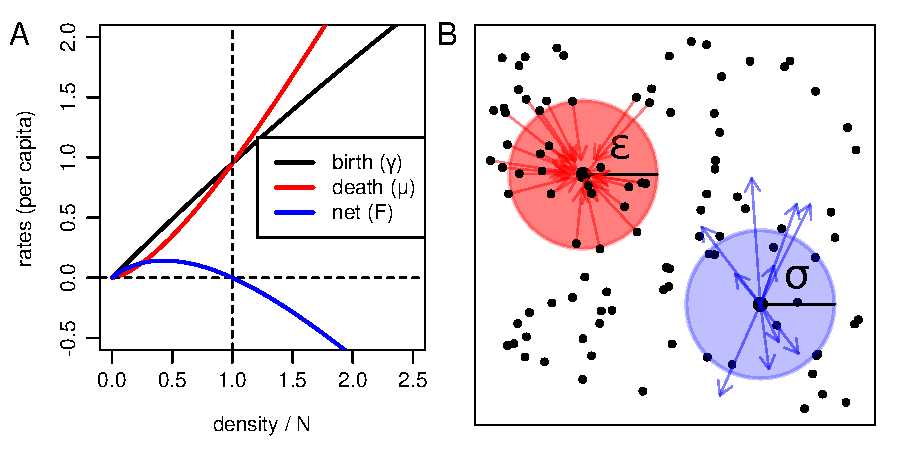
\includegraphics{figures/conceptual_figure}
    \end{center}
    \caption{
        Conceptual figure of the model.
        \textbf{(A)} Example plot of $\gamma$, $\mu$, and $F$
        (calculated with $r=1$) against scaled local population density.
        In this example, both birth and death rates increase with population density,
        but death increases faster,
        and equilibrium occurs where they cross
        (and hence where $F=0$).
        \textbf{(B)} Cartoon of interaction ($\epsilon$) and dispersal ($\sigma$) distances.
        \label{fig:model_setup}
    }
\end{figure}

Birth, establishment, and death can depend on the location of the individual
and the local population density.
Since we would like the population density to scale with $N$,
these are functions of $X/N$, i.e.,
the counting measure with mass $1/N$ placed at the location of each individual.
To measure local population density, we convolve the population measure with
an ``interaction kernel'' -- for simplicity, we take these to be Gaussian
with various scales, and write
$$
    p_{\sigma^2}(x) = \frac{1}{(2 \pi \sigma^2)^{d/2}} e^{-\|x\|^2 / 2 \sigma^2} .
$$
Given a nonnegative function $\gamma(x, m) : \IR^d \times \IR_{\ge 0} \to \IR_{\ge 0}$,
the birth rate of an individual at location $x$ when the state of the population is $X$
is $\gamma(x, \smooth{\gamma} X(x) / N)$,
where $\smooth{\gamma} X$ is the convolution of $X$
with $p_{\epsilon_\gamma^2}$.
Similarly, the establishment probability of an offspring at location $x$ is
is $r(x, \smooth{r} X(x) / N)$,
where $r(x, m) : \IR^d \times \IR_{\ge 0} \to [0, 1]$
and again $\smooth{r} p_{\epsilon_r^2}$.
Rather than defining a function $\mu(x, m)$ for the death rate,
it turns out to be more convenient to parameterize in terms of the net reproductive rate,
which we denote by $F(x, m)$,
scaled by $1/\theta$
so that the population density changes over a time scale of $\theta$,
i.e., we have ``near-critical branching''.
Informally, we would like that
$$
    F = \theta (r \gamma - \mu) ,
$$
and to arrange this we define
the death rate of an individual at $x$ to be
\begin{align} \label{eqn:mu_defn}
    \mu
    =
    \max\left\{0, 
        r(x, \smooth{r} X(x) / N) \gamma(x, \smooth{\gamma} X(x) / N)
        - \frac{1}{\theta} F(x, \smooth{F} X(x) / N)
    \right\} ,
\end{align}
where again $F(x, m) : \IR^d \times \IR_{\ge 0} \to \IR_{\ge 0}$
and $\kernel_F = p_{\epsilon_F^2}$.

In summary, demographic parameters depend on local density measured
for birth over a scale of $\epsilon_\gamma$,
for establishment over a scale of $\epsilon_r$,
and for net reproductive rate over a scale of $\epsilon_F$.
Note that death rates depend in principle on population densities at three different scales,
so that we could write $\mu = \mu(x, \smooth{\gamma} X(x) / N, \smooth{r} X(x) / N, \smooth{F} X(x) / N)$.
It might seem like
we have introduced unnecessary complexity
with these three different spatial scales on which interactions occur.
However,
it will turn out to be useful in the proofs to have $\epsilon_r < \epsilon_\gamma$,
although in the limit they can be taken equal to each other,
so informally we think of local density as being determined on a scale of $\epsilon$.
The value of $\epsilon_F$ is unconstrained.

\begin{remark}
Although this model allows fairly general birth and death mechanisms,
there are a number of limitations.
Perhaps most obviously, to simplify the notation
individuals give birth to only one offspring at a time,
although this restriction could be easily lifted
\citep[as in][]{etheridge/kurtz:2018}.
Furthermore, individuals do not move during their lifetime,
and the age of an individual does not affect their fecundity or death rates.
Finally, there is no notion of mating,
so availability of mates will not restrict the spread of a population,
and the lineages we follow will be uniparental.
For these reasons, the model is most obviously applicable to bacterial populations,
although we do not anticipate that incorporation of these complications
will change the general picture.
\end{remark}

We next summarize the dynamics of the rescaled model $\eta(t) = X(\theta t)/N$,
and state some assumptions on the parameters.

\begin{definition}[Model parameterization and assumptions]
    \label{def:model_setup}
    For each $\theta \ge 0$,
    let $\left(\eta^\theta(t)\right)_{t \ge 0}$
    be the continuous-time measure-valued Markov process described above
    with birth rates, establishment probabilities, and death rates
    determined as follows.
    Suppose $\gamma(x, m)$, $r(x, m)$, and $F(x, m)$
    are bounded, uniformly continuous functions
    from $\IR^d \times \IR_{\ge 0}$ to $\IR_{\ge 0}$.
    Furthermore, suppose $r$ takes values in $[0, 1]$
    and has uniformly bounded second derivatives,
    and that $(x, m) \mapsto m^2 \gamma(x, m)$ is unformly bounded.
    Fix nonnegative values $\epsilon_r$, $\epsilon_\gamma$, and $\epsilon_F$,
    with $\epsilon_r < \epsilon_\gamma - 1/\theta$.
    Suppose $F: \IR^d \times \IR_{\ge 0} \to \IR$ is bounded and uniformly continous
    and define
    \begin{align} \label{eqn:mu_defn}
        \mu(x, \eta)
        =
        r(x, \smooth{r} \eta(x))
        \gamma(\smooth{\gamma} \eta(x))
        - \frac{1}{\theta}
        F(x, \smooth{F} \eta(x)) .
    \end{align}
    Let $N$ be a positive number determined by $\theta$.
    When the state of the process is $\eta$,
    offspring of mass $1/N$ are produced at location $x$
    with rate $\theta \gamma(x, \smooth{\gamma} \eta^{\theta}(x)) N \eta^{\theta}_s(dx)$
    and adults die at location $x$ with rate $\theta \mu(x, \eta) N \eta^{\theta}_s(dx)$,
    (i.e., at rates $\theta \gamma$ and $\theta \mu$ per capita respectively).
    Offspring disperse to a location offset from the parent's location
    by an independent Gaussian with mean $\meanq/\theta$
    and covariance matrix $\covq / \theta$;
    an offspring at $x$ establishes instantaneously
    with probability $r(x, \smooth{r} \eta^{\theta}(x))$, or else dies.
\end{definition}

We will now define $(\eta^{\theta}(t))_{t \geq 0}$
explicitly as a solution to a Martingale problem.

\begin{definition}[Martingale Problem Characterisation]
    \label{Def: Rescaled Models}
We define $(\eta^{\theta}_t)_{t \geq 0}$ to be the solution to the Martingale Problem,
with initial condition $\eta^{\theta}_0$,
such that for all smooth functions $f \in C^{2}_{0}(\mathbb{R}^d)$,
\begin{equation}
    \label{eq: Pre-limit Martingale Characterisation}
\begin{aligned}
M^{\theta}_t(f)
&:=  \langle f,\eta^{\theta}_t \rangle
        -\langle f,\eta^{\theta}_0 \rangle
 \\ &\qquad {}
 -  \int_{0}^{t}\bigg\{
        \int\left(   \int \theta
     \left(
        f(z)r\big(z,\rho_{r}*\eta^{\theta}_{s}(z)\big)
            -f(x)r\big(x,\rho_{r}*\eta^{\theta}_{s}(x)\big)
            \right)
                    q_\theta(x,dz)\right)
        \\ & \qquad \qquad \qquad \qquad {} \times
                            \gamma\big(x,\rho_{\gamma}*\eta^{\theta}_{s}(x)\big)
                            \eta^{\theta}_{s}(dx)
     \\ & \qquad \qquad {} +\int 
     f(x)F\big(x,\rho_{F}*\eta^{\theta}_{s}(x)\big)
     \eta^{\theta}_{s}(dx)
    \bigg\} ds
\end{aligned}    
\end{equation}
is a martingale with quadratic variation
\begin{equation}
\begin{aligned} \relax
[ M^{\theta}_t(f)] =& 
\frac{\theta}{N} \int_{0}^{t}\bigg\{
\langle \gamma\big(x,\rho_{\gamma}*\eta^{\theta}_{s}(x)\big)
\int f^2(y)r\big(y,\rho_{r}*\eta^{\theta}_{s}(y)\big)q_\theta(x,dy) 
,\eta^{\theta}_{s}(dx)\rangle\\
& \qquad \qquad +\langle \mu\big(x,\eta^{\theta}_{s}\big)f^2(x) 
,\eta^{\theta}_{s}(dx)\rangle \bigg\}ds. 
\end{aligned}    
\end{equation}


\end{definition}

Since we are taking a diffusion limit,
we will have use for the following notation:

\begin{definition}[Dispersal generator]
    \label{def:dispersal_generator}
    Recall that we have defined the dispersal kernel,
    $q_\theta(x, dy)$,
    to be the density of a multivariate Normal
    with mean $\meanq/\theta$ and covariance matrix $\covq/\theta$.
    This implies that if we define, for $f : \IR^d \to \IR$,
    \begin{align}
    \DG f(x) = \sum_i \meanq_i \partial_{x_i} f(x)
        + \sum_{ij} \covq_{ij} \partial_{x_i} \partial_{x_j} f(x)
    \end{align}
    then
    \begin{align}
        \theta \int \left(
            f(y) - f(x)
        \right) q_\theta(x, dy)
    \to \DG f(x) 
        \qquad \text{as } \theta \to \infty .
    \end{align}
\end{definition}

\paragraph{Remark:}
An equivalent way to describe the model
would be to say that an individual at $x$ gives birth at rate
$$
    \gamma(x, \smooth{\gamma} \eta(x))
    \int r(x, \smooth{r} \eta(y)) q(x, dy) ,
$$
and that offspring disperse according to the kernel
$$
    q_\theta^\mathfrak{m}(x, dy)
    :=
    \frac{
        r(y, \smooth{r} \eta(y)) q_\theta(x, dy)
    }{
        \int r(x, \smooth{r} \eta(z)) q_\theta(x, dz)
    } .
$$
Clearly, the random walk driven by this dispersal kernel
should be biased towards regions of higher establishment probability.
For comparison to future results,
it is interesting to write down the limiting generator:
\begin{align*}
    \lim_{\theta \to \infty}
    \theta \int (f(y) - f(x)) q_\theta^\mathfrak{m}(x, dy)
    &=
    \frac{
        \DG\left[ f(\cdot) r(\cdot, \smooth{r} \eta(\cdot)) \right](x)
        - 
        f(\cdot) \DG\left[ r(\cdot, \smooth{r} \eta(\cdot)) \right](x)
    }{
        r(x, \smooth{r} \eta^{\theta}(x))
    } .
\end{align*}
In the simplest case of unbiased, isotropic dispersal,
$\meanq = 0$ and $\covq = I$, so $\DG = \Delta$,
and this is equal to
\begin{align*}
    \Delta f(x) + 2 \grad f(x) \cdot \grad \log r(\cdot, \smooth{r} \eta(\cdot))(x) .
\end{align*}
However, we will see that following a lineage back through the population
has a different behavior yet again.


% % % % % % % % % % % % % % %
\subsection{Main results on population processes}

\comment{
Set-up: there are two dichotomies:
is the limiting process deterministic or a generalized superprocess?
See Figure \ref{fig:super_vs_det_2d} for simulations.
And, are interactions local in the limit or not?
Below we have results for three of these cases;
as for the remaining one (local, superprocess),
it should be possible in 1D, not in higher dimensions (brief note).
}


\begin{figure}
    \begin{center}
        FIGURE
    \end{center}
    \caption{
        TODO: Figure depicting deterministic vs superprocess dichotomy:
        showing 2D images of populations,
        one with $\theta/N$ not small, the other with $\theta/N$ small.
        \label{fig:super_vs_det_2d}
    }
\end{figure}

\begin{theorem} \label{thm:nonlocal_convergence}
    Let $(\eta^\theta_t)_{t \geq 0}$
    be as defined in Definition \ref{def:model_setup}
    and assume that as $\theta \to \infty$, $N \to \infty$
    in such a way that $\theta/N \to \alpha$.
    (However, interaction distances $\epsilon_r$, $\epsilon_\gamma$, and $\epsilon_F$
    remain constant.)

    The sequence of stochastic processes
    $(\eta^\theta_t)_{t \geq 0}$
    converges along subsequences in distribution as $\theta \to \infty$
    to a measure-valued process $(\eta_t)_{t \geq 0}$
    which satisfies that, for every $f:\mathbb{R}^d \rightarrow \mathbb{R}$,
    \begin{align} \label{eqn:mgale_problem}
        M_t
        &:=
        \langle f(x), \eta_t(dx) \rangle
        -
        \langle f(x), \eta_0(dx) \rangle
        \\ & \qquad
        -
        \int_0^t \big\langle
            \gamma(x, \smooth{\gamma} \eta_{s}(x))
            \mathcal{B}\left(
                f(\cdot) r(\cdot, \smooth{r} \eta_{s}(\cdot))
            \right)(x)
            +
            f(x)
            F(x, \smooth{F} \eta_{s}(x)),
            \eta_{s}(dx)
        \big\rangle ds,
    \end{align}
    is a martingale.
    The quadratic variation of $M_t$, denoted $\langle M \rangle_t$, is given by 
    \begin{align} \label{eqn:mgale_variation}
        \langle M \rangle_t
        =
        \alpha
        \int_0^t
        \big\langle
            \gamma\left( x, \smooth{\gamma} \eta_{s}(x) \right)
            r\left(x, \smooth{r} \eta_{s}(x) \right)
            f^2(x),
            \eta_{s} (dx)
        \big\rangle ds. 
    \end{align}
    In other words, the limit is a measure-valued process with non-local interactions.
    Furthermore, if $\alpha = 0$ the limit is deterministic.
\end{theorem}

Theorem \ref{thm:nonlocal_convergence} provided convergence along subsequences;
i.e., for any sequence of values of $\theta$
there is a subsequence that converges.
However, if the limiting process is unique then the convergence is unqualified.
In the deterministic case, we have convergence to a nonlocal PDE.
\comment{Maybe the following two corollaries should be combined?}

\comment{
TODO: insert definition of "weak solution of the PDE \ref{eqn:nonlocal_pde}" heere.
}

\begin{corollary}[Deterministic limits]
    \label{cor:nonlocal_pde_limits}
    \comment{(TODO: remove "has a density" and rephrase appropriately)}
    In the context of Theorem~\ref{thm:nonlocal_convergence},
    if the limit is deterministic (i.e., $\theta / N \to \alpha = 0$), $\eta_0$ has a density,
    and \comment{additional conditions? can we say something like this??}
    then any limit $\eta_t(dx)$ has a density $\varphi(t, x)$,
    which is a weak solution to the nonlocal partial differential equation
    \begin{equation} \label{eqn:nonlocal_pde}
        \partial_t \varphi(t, x)
        =
        r\left(x, \smooth{r} \varphi(t,x) \right)
        \mathcal{B} \left[
            \varphi(t, \cdot)
            \gamma\big( x, \smooth{\gamma} \varphi(t, \cdot) \big)
        \right](x)
        +
        \varphi(t, x)
        F\left(x, \smooth{F} \varphi(t,x) \right)
        .
    \end{equation}
    If equation \eqref{eqn:nonlocal_pde} has a unique solution,
    then $(\eta^\theta_t)_{t \ge 0}$ converges to that solution.

    In particular, if
    \comment{TODO: find some conditions under which this is true?}
    then we have convergence to a unique solution.
\end{corollary}

Informally, equation \eqref{eqn:nonlocal_pde} is the PDE
\begin{align} \label{eqn:pde}
    \dot \varphi = r \DG\left( \gamma \varphi \right) + \varphi F ,
\end{align}
where $\DG$ is an elliptic second order differential operator,
and the coefficients $r$, $\gamma$, and $F$
at $x$ depend nonlocally on $\varphi$
(i.e., through a smoothed version of $\varphi$).

\comment{TODO: Tom has conditions (coefficient are Lipschitz?) under which
    the solution to \eqref{eqn:nonlocal_pdf} has a density (Thm 2.1 in DDMOT);
    should we insert those here (as a Corollary or Proposition, maybe?)}

\begin{corollary}[Superprocess limits] \label{cor:superprocess_uniqueness}
    In the context of Theorem~\ref{thm:nonlocal_convergence},
    if the martingale problem
    defined by equations \eqref{eqn:mgale_problem} and \eqref{eqn:mgale_variation}
    has a unique solution,
    then $(\eta^\theta(t))_{t \ge 0}$ converges to that solution
    as $\theta \to \infty$.
    \comment{
        Is this what we want to say here? Could be said better.
        TODO: see what Dawson \& Li say about uniqueness
        so we have at least some conditions under which this happens.
    }
\end{corollary}

Theorem~\ref{thm:nonlocal_convergence} shows convergence to the solution to a nonlocal PDE
of the form \eqref{eqn:nonlocal_pde}.
Since the coefficients at $x$ in \eqref{eqn:nonlocal_pde}
depend only on the region nearby to $x$,
we would often expect solutions of the nonlocal PDE to be close to the corresponding local PDE
as the interaction distances $\epsilon_r$, $\epsilon_\gamma$ and $\epsilon_F$
go to zero.
The following propositions give two concrete situations in which that is true.

\comment{I've not got straight exactly how we're framing this
    (namely, does $\eta$ have a density?).
    Also, is this one or two propositions --
    we said initially this would be two,
    one for FKPP and one for PME,
    but then maybe the argument was more general?
}

\begin{proposition}
    \label{prop:nonlocal_to_local}
    Suppose that $\eta_\epsilon(t,dx)$ is a solution to equation \eqref{eqn:nonlocal_pde}
    with $r(x, m) = 1$ for all $x$ and $m$
    and some $\epsilon_r < \epsilon_\gamma = \epsilon_F = \epsilon$
    \comment{and assumptions on $\gamma$? and $F$?}.
    Then $\eta_\epsilon(t, dx)$ converges \comment{in what sense?} as $\epsilon \to 0$
    to $u(t, x) dx$, which solves
    \begin{align} \label{eqn:PDE}
        \partial_t u(t, x)
        =
        \DG \left( \gamma(\cdot, u(t, \cdot) u(t, \cdot)  \right)(x)
        + F(x, u(t, x)) u(t, x) .
    \end{align}
\end{proposition}

Theorem \ref{thm:nonlocal_convergence} combined with Proposition \ref{prop:nonlocal_to_local}
imply that we can take the $\theta \to \infty$ limit
followed by $\epsilon \to 0$
to obtain solutions to the PDE \eqref{eqn:PDE}.
However, it is of substantial interest to know whether
we can take those two limit simultaneously.
The general case seems difficult,
but we can prove such ``diagonal'' convergence in the following situation.

\begin{theorem}[Convergence to a PDE]
    \label{thm:local_convergence}
    Let $(\eta^\theta_t)_{t \geq 0}$
    be as defined in Definition \ref{def:model_setup}
    and assume that as $\theta \to \infty$, $N \to \infty$
    and $\epsilon_r < \epsilon_\gamma = \epsilon_F = \epsilon \to 0$
    in such a way that $\theta/N \to 0$
    and
    \comment{TODO: some conditions on $\epsilon$ and $r$ and $\gamma$ and $F$}.
    Then the sequence of stochastic processes $(\eta^\theta_t)_{t \ge 0}$
    converges \comment{in some sense}
    to a measure-valued process with a density $\varphi(t, x)$
    that solves
    \begin{align}
        \partial_t \varphi(t, x)
        &=
        \text{whatever the final form is here} .
    \end{align}
\end{theorem}


% % % % % % % % % % % %
\subsection{Main results on lineages}

Now that we have established what we can say about how population density changes with time,
we turn to results on ancestral lineages,
i.e., how genealogical ancestry moves across the landscape.
Informally,
a \emph{lineage} $(L_t)_{t \ge 0}$
begun at spatial location $L_0 = x$
can be obtained by picking a focal individual uniformly at $x$,
and then for each amount of time $t$ in the past,
setting $L_t$ to the spatial location of the individual from whom
the focal individual inherits.
Since in our model individuals have only one parent, this is unambiguous.
Although we did not explicitly retain such information,
it is clear that
for finite $\theta$ (and hence, finite $N$),
one could construct the distribution of a lineage $(L_t)_{t=0}^T$
given the history of the population $(\eta^\theta_t)_{t = 0}^T$,
for each starting location to which $\eta^\theta_T$ assigns positive mass.
It is less clear, however, how to formally retain such information in the limit.
The \emph{lookdown construction} in Section~\ref{sec:lookdown}
provides just such a construction,
where lineages are retained in the $N \to \infty$ limit.
Roughly speaking,
this works by assigning to each particle a unique ``level''
that functions as a label and thus allows reconstruction of lineages,
but also (in some sense) orders individuals by eventual reproductive output,
allowing a formal limit.
See~\ref{etheridge/kurtz:2018} for an introduction to these ideas.

A lineage is, in general, a well-defined stochastic process,
but there are two important questions
that affect its tractability.
First, when is it a Markov process given the population process?
(I.e., given $(\eta_t)_{t=0^T}$ that records numbers of individuals
but not their ancestry.)
We expect the answer here to be that a lineage is Markov
only in the $N \to \infty$ limit.
\comment{(or, do we know this? we can cite Barton, Depaulis and Etheridge at least for discussion.)}
Second, does the process have a tractable description?
If the population process has a density,
then it turns out that a lineage is a diffusion driven by the density.
The remaining case is the superprocess limit ($\theta/N \to \alpha > 0$);
in this case, we expect that a lineage could still be described as a generalized diffusion,
but moving within a stochastic landscape that is singular in $d \ge 2$.
We focus on the more tractable situation where the population process is deterministic.
However, the results here apply to either the local or nonlocal case
(i.e., where the density solves a local or nonlocal PDE).

\comment{
    \textbf{Note:} the previous write-up motivated things only in the time-stationary case
    (so, a stationary traveling wave, possibly with wave speed zero;
    see the corollary below).
    It'd be very nice to give this more general result,
    but the proof has to be checked to make sure it still applies,
    and the notation is time-inhomogeneous and so more annoying
}


\begin{definition}[Generator of a lineage] \label{def:lineage_generator}
    Let $(\varphi(x, t))_{0 \le t \le T}$
    denote the density of a population that solves \eqref{eqn:nonlocal_pde},
    and let $y$ be a point with $\varphi(y, T) > 0$.
    We define $(L_s(y))_{s=0}^T$,
    the ancestral lineage of an individual sampled at $y$ at time $T$,
    to be the position of the unique ancestor of $y$ alive at time $T - s$.
    We define
    $(Q_s)_{s \geq 0}$
    to be the time inhomogeneous semi-group satisfying
    \begin{align*}
        Q_s f(y) := \IE_y[ f(L_s) ] ,
    \end{align*}
    and $\Lgen_s$ to be the generator of this semi-group.
\end{definition}

Our main result identifies a lineage as a diffusion
by characterizing its generator.
To avoid complexity,
we do this in the case where dispersal is $N(\meanq/\theta, \sigma^2 I/\theta)$,
in which case $\DG = \sigma^2 \Delta + \meanq \cdot \grad$.

\comment{
    Allowing a more general dispersal mechanism won't just entail replacing $\Delta$ with $\DG$,
    it will also change at least one of the $\grad$s to something else (I think).
}

\begin{theorem} \label{thm:lineages}
    In the context of Definition~\ref{def:lineage_generator},
    if the dispersal process is isotropic (i.e., $\covq = \sigma^2 I$),
    then
    \begin{equation}
        \label{eqn:lineage_generator}
        \Lgen_s f
        =
        \sigma^2 r \gamma
        \left(
            \Delta f
            +
            \left(
                2 \grad \log(\gamma \varphi)
                - \meanq
            \right)
            \cdot \grad f
        \right) .
    \end{equation}
    In other words, 
    a lineage behaves as a diffusion
    that is driven by a Brownian motion 
    run at speed $\sigma^2$ multiplied by the local per-capita production of offspring ($r \gamma$)
    in a potential equal to the local birth output tilted by migraiton bias
    ($\varphi \gamma \exp(-\meanq \cdot x / 2 \sigma^2)$).
\end{theorem}

To make the generator readable, we've written it in concise notation,
omitting the dependencies on location and population density,
which itself changes with time.
When interpreting this,
remember that everything depends on location and density at that location and time --
for instance, ``$r$'' is actually $r(x, \varphi(T-s, x))$.

\comment{This corollary was the previous theorem in the previous draft.
    Besides this proposed set-up, we have the additional options of
    (a) renaming the corollary a theorem and only proving it,
    or (b) presenting only the corollary here (as a theorem)
    and presenting the more general theorem later on.
}

\begin{corollary} \label{cor:wavefront}
    In addition to the assumptions of Theorem~\ref{thm:lineages},
    suppose that the population process is described by a traveling wave with speed $\wavespeed$,
    i.e., the population has density
    $\varphi(t, x) = w(x - t \wavespeed)$
    where $w$ solves
    \begin{align*}
        r \Delta (\gamma w) + w F(w) + \wavespeed \cdot \grad w = 0 .
    \end{align*}
    Then the generator $\Lgen$
    of the motion of a linages in this population is
    \begin{align}
        \Lgen f
        &=
        r \gamma
        \left(
            \Delta f
            +
            2 \grad \log (\gamma w)
            \cdot \grad f
        \right)
        + \wavespeed \cdot \grad f .
    \end{align}
\end{corollary}


%%%%%%%%%%%%%%%%%%%%%%
\section{Examples and applications}

Next,
we cover some illustrative examples
and interesting applications.

% % % % % % % % % % % %
\subsection{A nonlinear diffusive population: the Porous Medium Equation}

\comment{
    This section:
    model set-up including the limit;
    comparison of the simulation profile to deterministic solution.
    See Figure \ref{fig:pme_waves}.
}

Consider the porous medium equation (PME) with logistic growth,
\begin{equation}
    \label{eqn:pme}
    \partial_t v = \partial_x^2 (v^2) + v (1 - v) ,
\end{equation}
an example of a reaction-diffusion equation with a nonlinear diffusion term.
Such equations are widely used in a number of contexts in biology in which
it is clear that motility within a population varies with population density.
For example, density dependent dispersal is a common feature in spatial
models in ecology, eukaryotic cell biology, and avascular tumour growth;
see e.g.~\cite{sherratt:2010} and references therein for further discussion. 
We shall pay particular attention to the case in which the equation can be 
thought of as modelling the density of an expanding population. 
The specific equation that we use to illustrate the implications of
our results is one of a class used to study pattern formation in 
bacterial colonies. In particular, it has been suggested as a model for
the expansion of bacteria of the type {\em Paenbacillus dendritiformis} on
a thin layer of agar in a petri dish, 
\cite{cohen/golding/kozlovsky/benjacob/ron:1999}. 

Comparing \eqref{eqn:pme} to \eqref{eqn:pde},
we see that to set up a limit in which the population density $\varphi$ follows the PME,
we need $r=1$,
$\gamma = \varphi$, and $F = 1 - \varphi$.
Consulting equation~\eqref{eqn:mu_defn},
we then need death rate to be $\mu = (1 + 1/\theta) \varphi - 1/\varphi$.
In other words,
establishment is certain
and birth rates to increase linearly with population density,
but to compensate, death rates increase slightly faster (also linearly),
as shown in Figure~\ref{fig:pme_waves}.
Alert readers will notice that this violates our boundedness assumptions;
\comment{(perhaps this is too much detail here)}
in practice we choose a suitably small value for $\beta$ and define
\begin{align*}
    \gamma(x, m) &= (1 - \exp(- \beta m)) / \beta \\
    F(x, m) &= \exp(- \beta m) / \beta ,
\end{align*}
which in turn implies that death rate when local density is $m$
is roughly $(1 + 1/\theta) (1 - \exp(-\beta m)) / \beta - 1/(\theta \beta)$.
Birth and death rates are equal at density $m = 1$,
corresponding to an unscaled density of $N$ individuals per unit area.

\begin{figure}
    \begin{center}
        FIGURE
    \end{center}
    \caption{
        Two panels, showing simulated 1D populations under the PME, comparing the simulated
        profile to the analytical solution;
        $\theta/N$ not small on left; small on right.
        (Note: noisier wave should move slower, we'll see this.)
        \label{fig:pme_waves}
    }
\end{figure}

This equation has an explicit travelling wave solution
\begin{align} \label{eqn:pme_wave}
    w^P(t, x)
    :=
    \left( 1 - e^{ \frac{1}{2} (x - x_0 - t) } \right)_+ .
\end{align}
Notice that the wave profile has a sharp boundary at $x = x_0 + t$.
There are also travelling wave solutions with $c>1$ \citep{gilding/kersner:2005},
which lack this property.
However, for initial conditions that decay sufficiently rapidly at infinity,
such as one might use in modelling a population invading new territory,
the solution converges to \eqref{eqn:pme_wave} \citep{kamin/rosenau:2004}.

Indeed, simulations of this process
shown in Figure~\ref{fig:pme_waves}
display traveling wave solutions
similar to numerical solutions of the PME,
with increasingly good agreement for larger $\theta$ and $N$.
As expected, noise slows down the wave.


% % % % % % % % % % % %
\subsection{Traveling waves}

\begin{figure}
    \begin{center}
        FIGURE
    \end{center}
    \caption{
        Six panels: one pair for FKPP, one for PME, and one for Allen-Cahn.
        Each pair shows (top) lineage traced back in wavefront,
        and (bottom) stationary distribution of lineage location,
        compared to analytical solution for PME.
        \label{fig:pme_vs_fkpp}
    }
\end{figure}

\comment{
    This section:
    explain generator in stationary frame;
    derive stationary distribution;
    introduce FKPP;
    compute for PME and FKPP.
    (Also: Allen-Cahn example?)
    The two cases are very different, as shown in Figure \ref{fig:pme_vs_fkpp}.
}

It is interesting to investigate the motion of an ancestral lineage
in special cases in which we have an explicit expression for the travelling
wave profile $w$. 

%%%%%%%%%%
\paragraph{Porous Media:}
Setting $x_0=0$ (for definiteness) and substituting
the form of $w^P$ from equation \eqref{eqn:pme_wave}
into Corollary~\ref{cor:wavefront},
with $c=1$,
$\gamma(x, m) = m$,
$r(x,w) = 1$,
and $F(x, m) = (1 - m)$,
the lineage's generator is, for $x < 0$,
\comment{(need to decide whether to use $f_x$ or $\delta_x f$)}
\begin{align*}
    \Lgen f
    &=
        w(x)
        \left(
         f_{xx}
         +
         2 \frac{(w^2)_x}{w^2} f_x
        \right)
        + f_x \\
    &=
        \left(1 - e^{\frac{1}{2} x} \right)
        f_{xx}
        -
        2 e^{\frac{1}{2} x} f_x
        +
        f_x .
\end{align*}
The speed measure corresponding to this diffusion is,
again for $x < 0$,
\begin{align*}
    m(d\xi)
    &\propto
        \frac{ 1 }{ 2 (1 - \exp{\xi/2}) }
        \exp\left(
            \int_\eta^\xi \left\{
                1 - \frac{e^{x/2}}{1 - e^{x/2}}
            \right\} dx
        \right) \\
    &\propto
        e^\xi\left(1-e^{\xi/2}\right),
        \quad
        \text{for } \xi < 0 ,
\end{align*}
which is integrable and so when suitably normalised gives the unique stationary distribution.
Notice that at stationarity
the lineage will typically be significantly behind the front. 

%%%%%%%%%%
\paragraph{Fisher--KPP:}
A great deal more attention has been paid to the classical Fisher-KPP equation,
\begin{align} \label{eqn:fkpp}
    v_t = v_{xx} + v (1-v) .
\end{align}
In this case,
even though we do not have an explicit formula for the wave shape,
these methods give us information about ancestral lineages.
The equation has non-negative travelling wave solutions of speed $c$ for all $c \geq 2$, 
but started from any compact perturbation of a Heaviside function, the 
solution will converge to the profile $w^F$ with the minimal wavespeed, $c=2$,
\cite{kolmogorov/petrovsky/piscounov:1937,ramson:1983}.
No matter what the initial condition,
for any $t>0$ the support of the 
solution will be the whole real line. 
Since in ths case, $r = \gamma = 1$,
the generator of the motion of an ancestral lineage is
$$
    \Lgen \phi
    =
    \phi_{xx} + 2 \frac{w_x}{w} \phi_x + 2 \phi_x .
$$
Near the tip of the wave (for $x$ large), $w^F(x) \sim e^{-x}$,
so the motion of the lineage is close to Brownian motion.
On the other hand, for $x < 0$ the lineage behaves approximately as
Brownian motion with drift at rate two to the right.
This implies that
ancestral lineages are pushed into the tip of the wave,
and there is no stationary distribution.
These results agree with those of \comment{XXX}.


%%%%%%%%%%
\paragraph{Allen-Cahn:}
Finally, we take the Allen-Cahn equation
\begin{align} \label{eqn:allen_cahn}
    v_t = v_{xx} + v(1-v)(2v-1+s),
\end{align}
for a given $s \in (0,2)$,
which is used to model populations evolving under selection \cite{Sarah}.
This equation also has an explicit travelling wave solution
of shape
\[ w^A(x) = (1+e^{x})^{-1}. \]
The generator for ancestral lineages is, in this case,
\begin{align*}
    \hat{\mathcal{L}}\phi
    &=
    \phi_{xx}
    + 
    2 \frac{w_x}{w} \phi_x
    +
    s \nabla \phi \\
    \qquad &=
    \phi_{xx}
    -
    2 \frac{e^x}{1+e^x} \phi_x 
    + 
    s \nabla \phi,
\end{align*}
so lineages in the tip are pushed into the bulk of the wave by the drift $-2(e^{-x}+1)^{-1}$,
but that drift gets weaker further to the left.
This diffusion has speed measure
$$
    m(d\xi) \propto e^{sx}(1+e^x)^{-2},
$$
which is concentrated around $\log(s/(2-s))$ and decays like $e^{x(s-2)}$ away from this point.
These results agree with those of \cite{etheridge/penington:2020}.


% % % % % % % % % % % % % % % %
\subsection{Clumping from nonlocal interactions}

\comment{
    Description of the process;
    discussion of when it happens;
    (TODO: how's it affected by $\theta$?)
}

\begin{figure}
    \begin{center}
        FIGURE
    \end{center}
    \caption{
        Two panels: left is 2D picture of clumped population;
        right is a bumpy expanding wavefront.
        \label{fig:clumping}
    }
\end{figure}

% % % % % % % % % % % % % % % %
\subsection{Populations with Varying Lineage Distributions but Same Stationary Profile}

Consider two populations with coefficients $r_1, \gamma_1, \mu_1$ and  $r_2, \gamma_2, \mu_2$, and denote their lineage motion generator and profile as $\hat{\mathcal{L}}_1,w_1$, and $\hat{\mathcal{L}}_2,w_2$. We further assume that our populations have a stationary distribution with $\Xi_t(x)=w(x)$, i.e. $\mathfrak{c}=0$.\\
Let $\beta(x)>0$ and take $r_2(x)=r_1(x)\beta(x),~ \mu_2(x)=\mu_1(x)\beta(x),~ \gamma_2(x)=\gamma_1(x)$. Since $F=r\gamma-\mu$, we have that 
\begin{multline}
\label{eq: same profile scaled}
r_2\Delta(\gamma_2 w_2)+(r_2\gamma_2-\mu_2)(w_2)=0\implies r_1\beta \Delta(\gamma_1 w_2)+(r_1\beta \gamma_1-\mu_1 \beta)(w_2)=0\\
\implies r_1 \Delta(\gamma_1 w_2)+(r_1 \gamma_1-\mu_1)(w_2)=0 \implies w_2=w_1.
\end{multline}
The two populations share the same stationary profile but their ancestral lineage motions are different as 
\begin{equation}
\label{eq: different generator scaled}
\hat{\mathcal{L}}_2 \phi = r_1 \beta \gamma_1\left(\Delta\phi+2\frac{\nabla(\gamma_1 w_1)}{\gamma_1 w_1}\nabla\phi\right)\neq r_1 \gamma_1\left(\Delta\phi+2\frac{\nabla(\gamma_1 w_1)}{\gamma_1 w_1}\nabla\phi\right) = \hat{\mathcal{L}}_1 \phi.
\end{equation}
The stationary distribution of our population is unchanged when we scale $r,\mu$ by a rate of $\beta(x)$,
but the motion of lineages is sped up locally by $\beta$.
This corresponds to making areas with $\beta > 1$ more ``sink-like'',
because there death rate is higher, but also is the establishment of new individuals. Those regions as a result have lower long-term fitness and lineages spend less time there.


%%%%%%%%%%%%%%%%%%%%%%%%%
\section{Heuristics}
    \label{sec:heuristics}

\comment{TODO: short lead-in}

% % % % % % % % % % % % % % % % % %
\subsection{Population processes}
    \label{sec:population_heuristics}

We write $\Pgen^\theta$
for the generator of the scaled population process $\eta$ acting
on test functions of the form 
$$
    F( \langle f, \eta\rangle )
    =
    F \left( \int f(x)\eta(dx) \right),
$$
where $f \geq 0$ is smooth and compactly supported on $\IR^d$ and 
$F \in C^\infty ([0,\infty))$.
Recall that $N \to \infty$ along with $\theta$,
although we don't remind the reader with extra superscripts.


A Taylor expansion allows us to write
\begin{multline*}
    \Pgen^\theta
    F(\langle f,\eta \rangle)
    =
    F'(\langle f, \eta \rangle)
    \lim_{\delta t\downarrow 0} \frac{1}{\delta t}
    \IE\left[
        \left. \langle f, \eta_{\delta t} \rangle
        -
        \langle f, \eta \rangle
        \right| \eta_0=\eta
    \right]
    \\
    \qquad {}
    + \frac{1}{2}
        F''(\langle f,\eta\rangle)
    \lim_{\delta t\downarrow 0}\frac{1}{\delta t}
    \IE\left[
        \left.\big(\langle f,\eta_{\delta t}\rangle
        -
        \langle f, \eta\rangle\big)^2 \right|\eta_0=\eta
    \right]
    +
    \epsilon_{\theta}(f, F, \eta),
\end{multline*}
where the terms that make up 
$\epsilon_{\theta, N}(f, F, \eta)$
will be negligible in our scaling limit. 

% % % % % % % 
\subsubsection*{Mean measure}

Consider first the mean measure.
The birth rate at location $x$ when the state of the population is $\eta$
is a function of the location and the measure $\eta$ through a specific form:
$\gamma(x, \smooth{\gamma} \eta(x))$;
however, for the moment we will write $\gamma(x, \eta)$ instead
to make the exposition clearer
(and similarly for establishment probability $r(x, \eta)$ and death rate $\mu(x, \eta)$).
Recall that in our parameterization only $\mu$ and the dispersal kernel $q$ depend on $\theta$.
For a suitable (smooth, compactly supported) test function $f$, we find
\begin{equation} \label{mean measure}
    \begin{split}
    \Pgen^\theta \langle f, \eta \rangle
    &=
    \lim_{\delta t\downarrow 0} \frac{1}{\delta t}
    \IE\left[ \left.
        \langle f, \eta_{\delta t} \rangle
        -
        \langle f, \eta\rangle
        \right| \eta_0 = \eta
    \right]
    \\
    &=
    \theta \int
        \int f(z) r(z,\eta) q_\theta(x,dz)
    \gamma(x, \eta) \eta(dx)
    -
    \theta \int f(x)\mu_\theta(x, \eta)
    \eta(dx).
    \end{split}
\end{equation}
The first term is the increment in $\langle f,\eta\rangle$
resulting from a birth event (recalling that
we don't kill the parent) integrated against the rate of such events,
and the second reflects death events.
In both terms,
the rate of events has a factor of $N$ (because events happen at a rate 
proportional to the number of individuals,
whereas $\eta$ has mass $1/N$ for each individual)
which is offset by the fact that  
the birth or loss of a single 
individual at the point $y$, say, changes $\langle f,\eta\rangle$
by $f(y)/N$.

We use the fact that $\int q_\theta(x,dz)=1$ to rewrite~(\ref{mean measure})
as 
\begin{equation}
\label{eqn:rewritten mean measure}
\begin{split}
    \int\left(
        \int \theta \left( f(z) r(z,\eta)- f(x) r(x,\eta) \right) q_\theta(x,dz)
    \right)
    \gamma(x,\eta)
    \eta(dx)
    \\
    + \int \int f(x) \theta \Big(
        r(x,\eta) \gamma(x,\eta)
        - \mu_\theta(x,\eta)
    \Big) \eta(dx).
\end{split}
\end{equation}
We have defined $\mu_\theta$ so that the second term is simple:
\begin{align*}
    \theta \Big( r(x,\eta) \gamma(x,\eta) - \mu_\theta(x,\eta) \Big)
    = F(x, \eta) .
\end{align*}
This definition --
is really a `near-critical' assumption that birth and death rates
differ by something of order $1/\theta$.
Furthermore, since we've taken $q_\theta$ to be the density of a Normal
with mean and variance proportional to $1/\theta$,
\begin{align} \label{eqn:near_critical}
    \int \theta \Big(
        r(z,\eta) f(z)
        -
        r(x,\eta) f(x)
    \Big) q_\theta(x,dz) 
    \qquad \stackrel{\theta\to\infty}{\longrightarrow} \qquad  
    \DG \big(r(\cdot,\Xi)f(\cdot)\big)(x),
\end{align}
where recall if dispersal is simply standard multivariate Gaussian
with mean zero and covariance $\sigma^2 I / \theta$,
then $\DG = \sigma^2 \Delta$, where $\Delta$ denotes the Laplacian.
Note that there is a slight mismatch between the locations at which we are 
measuring birth and death rates, because in~\eqref{eqn:near_critical}
the establishment probability is 
measured at $x$ rather than at the point where juveniles fall. 

Equation~\eqref{eqn:rewritten mean measure}) then converges to
\begin{equation} \label{limit of mean measure equation}
\int \gamma(x,\eta)
\DG \big(f(\cdot)r(\cdot,\eta)\big)(x)
\eta(dx)
+
\int f(x)
F(x,\eta)
\eta(dx) .
\end{equation}
More generally, we expect everything to work
if the remaining parameters ($r$, $\gamma$, and $F$)
depended on $\theta$, but converged as $\theta \to \infty$.


% % % % % % % 
\subsubsection*{Quadratic variation}

% Note: this bit in firstversionplus.tex has things written out in detail for
% the Poisson offspring number case.

We now look at the second order term.
An individual at location $x$ gives birth 
to a surviving offspring at $y$ at rate
$$
\gamma(x,\eta) r(y,\eta) q_{\theta}(x, dy) ,
$$
and since this increments $\langle f, \eta \rangle$ by $f(y) / N$,
the contribution to the quadratic variation from birth events,
which occur at rate $\theta$ per individual 
(so, rate $N\theta |\eta|$ overall), is
$$
\langle
    N \theta \gamma(x,\eta)
    \int \frac{1}{N^2} f^2(y) r(y,\eta)
    q_\theta(x,dy) 
    , \eta(dx)
\rangle .
$$
Similarly, the increment in $\langle f, \eta\rangle$ resulting from 
the death of an individual at $x$ is $f(x)/N$, and so combining with the 
above, the second order term in the generator takes the form
$$
F''(\langle f,\eta\rangle)
\frac{1}{2} N \theta
\left\{
    \langle
        \gamma(x,\eta)
        \int \frac{1}{N^2}f^2(y)r(y,\eta)q_\theta(x,dy) 
    , \eta(dx)\rangle
    +
    \langle
        \mu_\theta(x,\eta)\frac{1}{N^2}f^2(x) 
    ,\eta(dx)\rangle
\right\} .
$$
The term $\epsilon_{\theta,N}(f, F, \eta)$ will be 
$\bigO(\theta/N^2)$.

% % % % % % % %
\subsubsection*{Limit I: deterministic case}

\comment{Need to decide what to call the limit here (and above, I guess).}

By choosing $\theta/N\rightarrow 0$, the second order term in the generator 
will vanish and we expect a deterministic limit. 
Let us suppose that the limit has a smooth density with respect to
Lebesgue measure, and abuse notation by using $\Xi_t(x)$
to denote the corresponding density, then integrating the first term in~(\ref{limit of mean measure equation})
by parts, we find that in the limit as $N\to\infty$,
\begin{equation*}
\frac{d}{dt}\int f(x)\Xi_t(x)dx
=
\int f(x)\left\{r(x,\Xi_t)\DG\big(\gamma(\cdot,\Xi_t)
\Xi_t(\cdot)\big)(x)
+
F(x,\Xi_t) \Xi_t(x)
\right\} dx.
\end{equation*}
In other words, we can expect the limit to be a weak solution to the 
deterministic equation
\begin{equation}
\label{deterministic limit}
\frac{d\Xi}{dt}
=r(x,\Xi)\DG\big(\gamma(\cdot,\Xi)
\Xi(\cdot)\big)(x)+F(x,\Xi)
\Xi(x).
\end{equation}


\subsubsection*{Limit II: stochastic case}

If $N=\alpha\theta$, for some positive constant $\alpha$,
the second order term in the generator remains order
one as $\theta\to\infty$, and  
we expect a `generalised superprocess' limit.
Assuming some regularity of the coefficients (in particular of $r$), 
the second order term in the generator will take the form
$$
\frac{1}{\alpha}F''(\langle f,\Xi\rangle)
\langle f^2(x), \gamma(x,\Xi)
r(x,\Xi)\Xi(dx)\rangle.
$$
That is
$$\langle f(x), \Xi_t(dx)\rangle-\langle f(x), \Xi_0(dx)\rangle
-\int_0^t\langle\gamma(x,\Xi_s)\DG\big(r(\cdot,\Xi_s)f(\cdot)\big)(x),
\Xi_s(dx)\rangle ds$$
is a martingale with quadratic variation
$$\frac{2}{\alpha}\int_0^t\langle f^2(x) 
\gamma(x,\Xi_s)r(x,\Xi_s),\Xi_s(dx)\rangle ds.$$




\plr{TODO: heuristics of conditions to get a local (PDE) limit?}


% % % % % % % % % % % % % % % % % %
\subsection{Lineages}

Although our proof of Theorem~\ref{thm:lineages}
uses the explicit representation in terms of the lookdown process,
informal calculations agree with the main result.
Suppose that we are tracking a lineage that is at location $y$ at time $t$.
Looking back through time, the lineage will move at the time that individual was born,
and will jump to the location of the parent of that individual.
Now, the rate at which new individuals are born to parents at $x$ and establish at $y$
is
$$
    \gamma(x, \eta_t) q(x, dy) r(y, \eta_t) .
$$
This implies that the probability a randomly chosen individual near $y$
is a new offspring from a parent at $x$ in $[t, t+dt)$ is, informally,
\begin{equation} \label{eqn:informal_rates}
\frac{
    \gamma(x, \eta_t) q_\theta(x, dy) r(y, \eta_t) \eta_t(dx)
}{
    \eta_t(dy)
} dt .
\end{equation}
Leaving aside questions of whether a lineage can be treated as a randomly chosen individual,
we might then proceed by defining a continuous-time jump process
whose transition rates are given by \eqref{eqn:informal_rates} given $(\eta_t)_{t=0}^T$.
Happily, we are interested in the case when $\eta$ has a density,
say $\eta_t(dx) = \varphi(x) dx$,
so interpreting these rates is not too difficult.
Now recall that $q_\theta(x, dy)$ is a Gaussian kernel
with mean $x + \meanq/\theta$ and covariance $\covq/\theta$.
Write $\widetilde q_\theta(y, dx)$ for the ``reverse-time'' distribution,
i.e., Gaussian with mean $x - \meanq/\theta$ and the same covariance.
Then, rearranging infinitesimals,
\eqref{eqn:informal_rates} implies a rate of
\begin{equation} \label{eqn:informal_rates2}
\frac{
    \varphi(x) \gamma(x, \eta_t) r(y, \eta_t)
}{
    \varphi(y)
} \widetilde q_\theta(y, dx) .
\end{equation}
Let $(L^\theta_s)_{s=0}^T$ be the location of a lineage that moves according to
jump rates~\eqref{eqn:informal_rates2},
back through time (i.e., with the substitution that $s = T-t$).
Then
\begin{align} \label{eqn:lineage_generator_Edt}
    \begin{split}
    &\IE[f(L^\theta_{s+ds}) \;|\; L_s = y] - f(y)
    \\&\qquad 
    =
    ds \int \left(f(x) - f(y)\right)
    \frac{
        \varphi_{T-s}(x) \gamma(x, \eta_{T-s}) r(y, \eta_{T-s})
    }{
        \varphi_{T-s}(y)
    }
    \widetilde q_\theta(y, dx) .
    \end{split}
\end{align}
Referring back to Definition~\ref{def:dispersal_generator},
recall that as $\theta \to \infty$,
$$
    \theta \int (f(x) - f(y)) \widetilde q_\theta(y, dx)
    \to
    - \sum_i \meanq_i \partial_{x_i} f(y)
    + \sum_{ij} \covq_{ij} \partial_{x_i x_j} f(y) ,
$$
which is just $\DG$ but with the first derivative terms multiplied by -1.
\comment{The $\widetilde \DG$ and $\covq \grad$ notation here is terrible; suggestions?}
Consequently,
\begin{align*}
    &
    \theta \int (f(x) - f(y)) g(x) \widetilde q_\theta(y, dx) \\
    &\qquad \to
    - g(y) \sum_i \meanq_i \partial_{x_i} f(y)
    + g(y) \sum_{ij} \covq_{ij} \partial_{x_i x_j} f(y)
    + \sum_{ij} \partial_{x_i} g(y) \covq_{ij} \partial_{x_j} f(y)  \\
    &\qquad =
    g(y) \widetilde \DG f(y)
    + (\covq \grad g) \cdot \grad f ,
\end{align*}
if we define $\widetilde \DG$ to be the same as $\DG$ but with $-\meanq$ substituted for $\meanq$,
and $(\covq \grad g(y))_i = \sum_j \covq_{ij} \partial_{x_j} g(y)$.
Applying this to~\eqref{eqn:lineage_generator_Edt} with $g = \varphi_{T-s} \gamma$,
this suggests that the generator of the limiting process is
\begin{align*}
    \Lgen_s f
    &=
    \frac{r}{\varphi_{T-s}}
    \left\{
        \varphi_{T-s} \gamma \widetilde \DG f
        + \left(\covq \grad (\varphi_{T-s} \gamma) \right) \cdot \grad f 
    \right\} \\
    &=
    r \gamma
    \left\{
        \widetilde \DG f
        + \left(\covq \grad \log(\varphi_{T-s} \gamma) \right) \cdot \grad f 
    \right\} .
\end{align*}
In other words, the lineage moves at speed equal to the local production of successful offspring,
$r \gamma$,
by a time-reversed version of the dispersal distribution,
but with a drift in the direction of the gradient of the logarithm
of the production of juveniles, $\grad \log(\phi_{T-s} \gamma)$
(modified by the covariance of dispersal).
This \comment{presumably?} agrees with \comment{the theorem}.


%%%%%%%%%%%%%%%%%%%
\section{The lookdown process}
    \label{sec:lookdown}


Now we will present a lookdown construction for the general process
(i.e., of Definition \ref{Def: Rescaled Models}),
in the spirit of~\cite{kurtz/rodrigues:2011}. 
The key benefit of this construction is that
we shall be able to preserve the notion of individuals,
and in particular their genealogies,
when we pass to the limit.


The gneral set-up is as follows.
Each individual will be labeled with a ``level'',
which will be a number in $[0, \lambda]$.
When taking the limit, we will set $\lambda = N$.
\comment{Should we just use $N$ instead of $\lambda$? Or vice-versa?}
We will still encode the process embellished by these levels
as a point measure:
if the $i^\mathrm{th}$ individual's spatial location is $x_i$
and level is $u_i$, then we will write:
$$
    \lp = \sum_i \delta_{x_i, u_i} ,
$$
which is a measure on $\IR^d \times [0, \lambda]$.
Note that the each individual contributes mass 1 to the measure,
not $1/N$ as above.
In some sense, these levels do not affect the process:
the pushforward of this measure-valued ``spatial-level process'',
divided by $N$,
will agree with the purely spatial process defined above.
Furthermore, the levels of the individuals present at any spatial location
conditionally uniform on $[0, \lambda]$.
However, an individual's level in some sense encodes their future reproductive output:
individuals with lower levels tend to live longer, and have more offspring.
For more explanation of the set-up and how this is possible,
see \citet{etheridge/kurtz:2018} and \citet{kurtz/rodrigues:2011}.
Furthermore, the limiting spatial-level process will still be a point measure,
and so we explicitly retain the notion of individuals and lineages through to the 
large-population-density limit.


% % % % % % % % % % % % % % % %
\subsection{Definition and generator of the lookdown process}
\label{sec:lookdown_defn}

In this section,
we'll define the process $(\lp_t)_{t \ge 0}$ in terms of the dynamics of labeled particles,
and write down it's generator.
Since the dynamics depend on the spatial locations of particles,
we \emph{define} $\eta_t$ to be the corresponding spatial measure,
i.e.,
$$
    \eta_t(\cdot) = \frac{1}{\lambda} \lp_t(\cdot \times [0, \lambda])  .
$$
A nontrivial consequence of the way we define $\lp_t$ will be that
this process has the same distribution as the process $(\eta_t)_{t \ge 0}$ defined above
in Definition~\ref{Def: Rescaled Models},
again, after setting $\lambda = N$.
(This provides our justification for using the same notation for both.)
Finally, note that we first describe the dynamics of individuals
in the original time units -- i.e., before scaling by $\theta$,
which will appear below.

\comment{
    I've defined $\eta = \lp / N$ to agree with how we define the generator below,
    for which birth/death add/remove something of mass 1, not $1/\lambda$.
}

\comment{TODO: this uses the $\gamma(x, \eta)$ notation, which we haven't settled on.}

Suppose that the initial population is composed of $O(\lambda)$ many particles
with levels uniformly distributed between $[0, \lambda]$.
Suppose the current state of the population is $\lp$,
with spatial projection $\eta$.
Each individual at spatial location $x$ with level $u$
produces one juvenile offspring at rate 
$$
2 \left(1 - \frac{u}{\lambda}\right) \gamma(x, \eta) ,
$$
which disperses to a location relative to $x$ drawn from the kernel $q(\cdot)$.
(Averaging over the uniform distribution of the level $u$,
we recover the birth rate $\gamma(x, \eta)$.)
This juvenile -- suppose it's location is $y$ --
either survives, with probability $r(y, \eta)$, or immediately dies.
(As before, ``maturity'' is instantaneous.)

A new level $u_1$ is sampled independently and uniformly from $[u,\lambda]$,
and the parent and the offspring are assigned in random order to the levels $\{u, u_1\}$.
This random assignment of levels to parent
and offspring ensures that conditional on $\eta$,
the levels of each individual at any point in time are independent, uniform random variables.

Evidently this mechanism increases the proportion
of individuals with higher levels.
To restore the property that,
conditional on $\eta$,
the distribution of levels is conditionally uniform,
we impose that 
the level of an individual at location $x$
evolves according to the differential equation
$$
    \dot{v}
    =
    % \gamma^{\mathfrak{m}}(x, \eta) \left\{\lambda^{-1}(\lambda -v)^{2} -(\lambda -v)\right\}.
    - \frac{v}{\lambda} \left(\lambda - v\right)
    \gamma(x, \eta) \int_{\IR^d} r(y, \eta) q(x, dy) .
$$
Since $v \in [0, \lambda]$, this moves levels down;
see~\cite{etheridge/kurtz:2018}, Section~3.4 for a detailed explanation.

In the lookdown model, levels never cross below 0,
while particles whose levels move above $\lambda$ are regarded as dead
(and do not affect to the population any more).
Therefore, in order to incorporate death,
the level of the individual at location $x$ with level $u$
moves upwards at an additional rate $\mu(x,\eta) u$.
Since levels are uniform,
it is easy to check that if $\mu$ was constant,
this would imply an exponential lifetime for each individual;
see~\cite{etheridge/kurtz:2018}, Section \comment{XXX}
for more general justification.

Putting these together,
the level $u$ of an individual at $x$ in $\lp$ evolves according to:
\begin{equation} \label{eqn:dot_u}
    \dot u
    =
    - \frac{\theta}{\lambda} u \left(\lambda - u\right)
    \gamma(x, \eta) \int_{\IR^d} r(y, \eta) q(x, dy) 
    +
    \theta \mu(x,\eta) u .
\end{equation}
The factor of $\theta$ appears here because we have rescaled time.
We shall write 
$$
    b(x, \eta)
    :=
    \theta\left(
    \gamma(x,\eta) \int_{\IR^d} r(y, \eta) q(x, dy)
    -
    \mu(x,\eta)
    \right) ,
$$
which captures the local net difference between reproduction and death,
i.e., the deviation from criticality of the branching mechanism.
Recall from equation \eqref{eqn:mu_defn} that
$F(x,\eta) = \theta(r(x,\eta)\gamma(x,\eta) - \mu(x,\eta))$,
and so we will have that
\begin{align} \label{eqn:b_limit}
b(x, \eta)
&=
    \theta \gamma(x, \eta) \int_{\IR^d} \left( r(y, \eta) - r(x, \eta) \right) q(x, dy)
    + F(x, \eta) \\
&\to
    \gamma(x, \eta) \DG r(x, \eta) + F(x, \eta) \qquad \text{as } \theta \to \infty .
\end{align}

We can then rewrite the differential equation 
governing how the level of each individual
in $\lp$ evolves as
\begin{align}
\dot{u}
    &=
    \theta \gamma(x,\eta) \int_{\IR^d} r(y, \eta) q(x, dy)
    \left\{
        -\frac{u}{\lambda}\left(\lambda - u\right)
        + u
    \right\}
    -
    b(x,\eta) u
    \nonumber \\
    &=
    \frac{\theta}{\lambda} \gamma(x,\eta) \int_{\IR^d} r(y, \eta) q(x, dy) u^2
    -
    b(x, \eta) u
    . \label{differential equation for level}
\end{align}
(The factor of $\theta$ appears because of the rescaling of time for $\lp$.)

Now, we can write down the generator for $(\lp_t)_{t \ge 0}$,
the lookdown process.
In what follows, we will write sums (and, products) over ``$(x, u) \in \xi$''
to mean as a sum over the (location, level) pairs of each individual in the population.
Test functions for $\lp$ then take the form
\begin{equation} \label{eqn:test_functions}
f(\lp)=\prod_{(x,u)\in \lp}g(x,u)=\exp\left(\int \log g(x,u)\lp(dx, du)\right),
\end{equation}
where
$g(x,u)$ is differentiable in $u$ and 
smooth in $x$.
We will also assume that $0\leq g(x,u) \leq 1$ for all $u\in [0,\lambda]$,
and $g(x,u)\equiv 1$ for $u\geq \lambda$.
In the expressions that follow,
we shall often see one or more factor of $1/g(x,u)$;
it should be understood that if $g(x,u)=0$,
then it simply cancels 
the corresponding factor in $f(\lp)$.

Recall also that in defining $\eta_t$
we had not only rescaled mass, dividing each individual's mass by $N$,
but also time, speeding up time by a factor of $\theta$.
As a result, per-capita rates described above will have a factor of $\theta$ here.

First consider the terms in the generator that come from birth events.
Recall that when a birth successfully establishes,
a new level is generated above the parent's level,
and this new level is assigned to either the offspring or the parent.
Since the probability of each is 1/2,
the contribution of birth to the generator is
\begin{align}
f(\lp) \nonumber
&\mapsto
    f(\lp)
    \sum_{(x, u) \in \lp}
    2 \frac{\theta}{\lambda} \gamma(x, \eta)
    \int_u^\lambda
    \int_{\IR^d}
    \left(
    \frac{1}{2}
    \bigg\{
            g(y, u_1)
        + \frac{ g(y, u) g(x, u_1) }{ g(x, u) }
    \bigg\}
        - 1
    \right)
    r(y, \eta) q(x, dy)
    \\
    \begin{split} \label{eqn:birth_generator}
&=
    f(\lp)
    \sum_{(x, u) \in \lp}
    2 \gamma(x, \eta)
    \bigg\{
        \frac{1}{2 \lambda}
        \int_u^\lambda
        g(x, u_1) du_1
        \frac{
            \theta \int_{\IR^d} (g(y, u) - g(x, u)) r(y, \eta) q(x, dy)
        }{
            g(x, u)
        }
    \\ & \qquad \qquad \qquad {}
        + \frac{\theta}{\lambda}
        \int_u^\lambda \int_{\IR^d}
        \left( \frac{g(y, u_1) + g(x, u_1)}{2} - 1 \right)
        r(y, \eta) q(x, dy)
    \bigg\}
    .
    \end{split}
\end{align}
Here, $u_1$ is the new level and $y$ is the offspring's location,
and so the two terms in the integral correspond to the two situations:
in the first, we have added an individual at $(y, u)$,
while in the second, we replace an individual at $(x, u)$
by one at $(x, u_1)$ and another at $(y, u)$.
We've written it in this form because the two pieces
each naturally converge to separate terns in the limit.

The remaining term in the generator is due to the motion of particles' levels:
\begin{align} \label{eqn:level_generator}
    f(\lp)
    \mapsto
    f(\lp)
    \sum_{(x, u) \in \lp}
    \left(
    \theta
        \lambda^{-1} \gamma(x,\eta) \int_{\IR^d} r(y, \eta) q(x, dy) u^2
        -
        b(x, \eta)u
    \right)
    \frac{\partial_u g(x,u)}{g(x,u)} .
\end{align}


\comment{TODO: consider whether this is where we stick in
    these explicit definitions of $\gamma$ and set $\lambda=N$.}
To scale our lookdown model to be consistent with
the spatial model described in \S \ref{sec: Model and main results},
we will let $\lambda$ takes on the role of $N$
in \S \ref{sec: Model and main results},
i.e. each individual has mass $1/\lambda$
in the scaling limit.
Time is once again scaled by $\theta$,
and the birth, death and establishment rates 
depend on local densities given by
mollification over Gaussian kernels with radius
$\epsilon_{\gamma}$, $\epsilon_{F}$ and $\epsilon_{r}$.

Explicitly, in the $\theta$-th stage of re-scaling,
an individual has mass $\frac{1}{\lambda} := \frac{1}{N}$
and a level between $[0,N]$;
the birth rate is
$$
    \gamma(x, \eta)
    :=
    \gamma(x, \smooth{\gamma}\eta(x)),
$$
the establishment probability is
$$
    r(x, \eta)
    :=
    r(x, \smooth{r}\eta(x)),
$$
the local branching mechanism $b(x,\eta)$ is 
$$
    b_{\theta}(x, \eta)
    :=
    \theta \left(
        \gamma(x, \smooth{\gamma}\eta(x))
        \int r(y, \smooth{r}\eta(y)) q_{\theta}(x,dy)
        -
        \mu(x, \eta)
    \right) .
$$
and the dispersal kernel is $q_\theta$.

We can now define the spatial-level process
explicitly as a solution to a Martingale Problem,
whose generator is just the sum of
\eqref{eqn:birth_generator} and \eqref{eqn:level_generator}.

% % % % % % % %
\begin{definition}[Martingale Problem Characterisation]
    \label{defn:lookdown_mgale}
We define $(\lp^{\theta}_t)_{t \geq 0}$
to be the (unique) solution
    \comment{(I'm not sure why unique is in parentheses here?)}
to the Martingale Problem
with initial condition $\lp_0 \in \mathcal{M}_F(\mathbb{R}^d \times [0,N])$
and generator $A^{\theta}$ that satisfies
\begin{equation*}
\begin{split}
& A^{\theta}f(\lp ) \\
&\quad =
    f(\lp)
    \,\sum_{(x,u)\in \lp}\,
    2 \gamma(x, \eta)
    \Bigg\{ \frac 12 N^{-1}\int_u^N g(x,u_1) du_1
            \times
            \frac{
                \theta \int_{\mathbb{R}^d}
                (g(y,u) - g(x,u))
                r(y, \eta) q_{\theta}(x,dy)
            }{ g(x,u) }
        \\
    &\qquad\qquad\qquad\qquad\qquad\qquad\qquad {} +
        N^{-1}\theta\int_u^N
        \int_{\mathbb{R}^d}\left(
            \frac{ g(y,u_1) + g(x,u_1) }{ 2 } - 1
        \right)
        r(y, \eta) q_{\theta}(x,dy)
        du_1
    \Bigg\}\\
    &\qquad\qquad {} +
    f(\lp) \sum_{(x,u)\in\lp}\,
    \left(
        \theta N^{-1} \gamma(x,\eta) \int_{\IR^d} r(y, \eta) q_\theta(x, dy) u^2 -b_{\theta}(x,\eta)u
    \right)
    \frac{\partial_u g(x,u)}{g(x,u)}
    ,
\end{split}
\end{equation*}
for all smooth functions $g \in C^{2}_{0}(\mathbb{R}^d)$,
where $f(\lp) = \prod_{(x, u) \in \lp} g(x, u)$ as defined in \eqref{eqn:test_functions},
and $\eta(\cdot) = \lp(\cdot \times [0, N]) / N$ is the spatial pushforward of $\lp$,
as before.
\end{definition}


In Appendix \ref{sec: Markov Mapping Theorem Application},
we will show that
if we define $\Gamma (d\textbf{u})$
as the probability kernel that corresponds to
assigning each particle an i.i.d. uniform $[0,N]$-level,
and for any $\lp \in \mathcal{M}_f(\mathbb{R}^d \times [0,\infty))$, we denote
$$\hat{f}(\lp)=\int f(\lp) \Gamma (d\textbf{u})$$ 
to be the spatial test functions with averaged level,
then the process
\begin{equation}
\begin{aligned}
M^{\theta}_t:=&\hat{f}(\lp_t)-\hat{f}(\lp_0)-\int_{0}^{t}\int   A^{\theta}f(\lp_s)\Gamma(d\textbf{u})ds\\
:=&\hat{f}(\lp_t)-\hat{f}(\lp_0)-\int_{0}^{t}   \Pgen^{\theta}\hat{f}(\lp_s)ds
\end{aligned}    
\end{equation}
is a martingale.

By the Markov Mapping Theorem,
there exists a solution $(\xi^{\theta}_t)_{t \geq 0}$
to the Martingale Problem with generator $A^{\theta}$.
Furthermore,
the spatial projection of $(\xi^{\theta}_t)_{t \geq 0}$
shares the same law of $(\eta^{\theta}(t))_{t \geq 0}$,
i.e.
$$(\eta^{\theta}(t))_{t \geq 0}
\sim \left(\frac{1}{N}\sum\limits_{(X(t),U(t))\in \xi^{\theta}(t)} \delta_{X(t)}\right)_{t \geq 0},$$
and conditional on 
$(\eta^{\theta}(t))_{t \geq 0}$,
the levels of particles in $(\xi^{\theta}_t)_{t \geq 0}$
are i.i.d. uniformly distributed between $[0,N]$.

Theorem A.10 in \cite{kurtz/rodrigues:2011}
states that convergence of $(\eta^{\theta}_t)_{t \geq 0}$
to a conditionally Poisson system $(\xi_t)_{t \geq 0}$
with Cox measure $\Xi_t \times \Lambda$
is equivalent to convergence of
$(\eta^{\theta}_t)_{t \geq 0}$ to $(\Xi_t)_{t \geq 0}$.
As a result, it suffices for us to focus on
tightness of $(\eta^{\theta}_t)_{t \geq 0}$
and spatial convergence of $(\eta^{\theta}_t)_{t \geq 0}$
as $\theta \to \infty$.


%% %% %% %% %% %% %% %% %% %% %% %%
\subsection{Construction of individual lineages}

Although we will \comment{(later)} show convergece of the lookdown process
defined by Definition~\ref{defn:lookdown_mgale}
to a stochastic process in which individuals retain their identities,
it is convenient to construct the lookdown process
in a way that explicitly represents the motion of each individual and their offspring.
This will then make obvious how linages move in the limit.

We will construct the process using a Ulam-Harris indexing scheme,
which associates the outcomes of each branching event with a label obtained
by appending to the previous label.
To begin, we assign each extant individual a label from $\IN_{\ge 0}$.
Suppose an individual with label $a$ and level $u$ reproduces,
and as a result there are two individuals, one with level $u$ and one with a new level $u_1 > u$.
The parent individual, previously labeled $a$, might be assigned either level.
We will track chains of descendant individuals forwards through time
following levels, rather than individuals, and will call this a \emph{line of descent}.
So, after reproduction, we give a new label to \emph{only} the individual
that is given the new level $u_1$,
retaining the label $a$ for the individual with the old level $u$.
So, there is a unique label assigned at each birth event,
and it is assigned to the resulting individual with the higher level.
It would be possible to reconstruct individual identities along a line of descent
from this construction,
but we don't write this out.

Concretely, then: for each label $a$ in
$\labelspace = \bigcup_{k \ge 1} \IN_{\ge 1}^k$
let $\Pi_a$ be an independent Poisson process on $[0, \infty)^2 \times \IR_d \times \{0,1\}$.
The mean measure is a product of Lesbegue measure on the first two coordinates,
$q(0, \cdot)$ on $\IR^d$, and $(\delta_0 + \delta_1)/2$ on $\{0, 1\}$.
It will also be convenient
to suppose that for each label $a$ we have an enumeration of the points in $\Pi_a$,
so we may refer to ``the $j^\text{th}$ point in $\Pi_a$'',
although the precise order of this enumeration is irrelevant.
If $(t, v, y, \kappa)$ is the $j^\text{th}$ point in $\Pi_a$,
then $t$ will determine possible birth times,
$v$ will determine levels of the offspring,
$y$ will give the spatial displacement of the offspring relative to the parent,
$\kappa$ will be used to determine whether parent or offspring are assigned the new level,
and the new label produced, if any will be $aj$,
i.e., the label $a$ with $j$ appended (so, if $a \in \IN_{\ge 0}^k$ then $aj \in \IN_{\ge 0}^{k+1}$).
Each label $a$ has a birth time $\tau_a$,
when it is first assigned,
and a death time $\sigma_a$, when its level first hits $\lambda$.
For any $\tau_a \le t \le \sigma_a$ we denote by $X_a(t)$ and $U_a(t)$ the spatial location and level
of the individual carrying label $a$ at time $t$.
Now, since we have defined labels so that the level does not jump,
$U_a$ satistifies~\eqref{eqn:dot_u} for $\tau_a \le t \le \sigma_a$, i.e.,
\begin{equation*}
    \begin{split}
& U_a(t)
    =
    U_a(\tau_a) \\
&\qquad {}   
    + \int_{\tau_a}^{t}
    \left(
        \frac{\theta}{\lambda} \gamma(X_a(s),\eta(s))
        \int_{\IR^d} r(z,\eta(s)) q(X_a(s),dz) U_a(s)^2
        -
        b(X_a(s),\eta(s)) U_a(s)
    \right)
    ds ,
\end{split}
\end{equation*}
and, of course, $\sigma_a = \inf\{t \ge \tau_a : U_a(t) > \lambda\}$.

Potential reproduction events occur at times $\tau_a + s$
for each point $(s, v, y, \kappa) \in \Pi_a$.
We say `potential' since if the resulting level is greater than $\lambda$,
the event does not happen.
If this is the $j^\text{th}$ point in $\Pi_a$,
the new label is $aj$ and the (potential) new level is
\begin{equation*}
    U_{aj}(\tau_a + s)
    =
    U_a(\tau_a + s)
    +
    \frac{
        v
    }{
        2 \lambda^{-1} \theta \gamma(X_a(\tau_a + s-), \eta(\tau_a + s-))
        r(X_a(\tau_a + s-) + y, \eta(\tau_a + s-))
    }.
\end{equation*}
If $U_{aj}(\tau_a+s) < \lambda$,
the new individual labeled $aj$ is produced,
and $\kappa$ determines which label is associated with the new location,
so
\begin{align*}
    X_{aj}(\tau_a + s)
    &=
    X_a(\tau_a+s-) + (1 - \kappa) y \\
    X_a(\tau_a+s)
    &=
    X_a(\tau_a+s-) + \kappa y .
\end{align*}
If $U_{aj}(\tau_a+s) \ge \lambda$, then $X_a$ is unchanged.
Recall that the parental \emph{individual} always retains their spatial location,
so that $\kappa = 0$ corresponds to the parent being assigned a new level,
and our line of descent switching to the offspring.


Consequently, 
the \emph{line of descent}
leading from the initial generation
to any label $a \in \labelspace$
can be explicitly constructed as follows.
Supposed that $a = (a_1, a_2, \ldots, a_n) \in \IN^n$,
and for $1 \le k \le n$ let $(a)_k = (a_1, a_2, \ldots, a_k)$.
Then, let $\zeta_a(t)$ denote the counting process that records
which label is present in the line of descent at time $t$,
i.e., $\zeta_a(t) = \max\{k \ge 1 : \tau_{(a)_k} \le t\}$.
This then lets us define $X_a(t)$ all the way back to $t=0$
by setting $X_a(t) = X_{(a)_{\zeta_a(t)}}(t)$ (and, $U_a(t)$ similarly).
Now, we can explicitly write down the evolution of $U_a(t)$ and $X_a(t)$.

First, for each $1 \le k < n$
let $(s_k, v_k, y_k, \kappa_k)$ be the $a_{k+1}^\text{th}$ point in $\Pi_{(a)_k}$
(this is the sequence of jumps taken by the line of descent).
Note that $s_k = \tau_{(a)_k}$, and also set $s_0 = 0$.
Let $\Gamma_a$ by the point process ``experienced by the line of descent leading to $a$'',
which is for $A \subset [0,\infty)^2 \times \IR^d \times \{0,1\}$
$$
\Gamma_a(A)
=
    \sum_{k=1}^n
    \Pi_{(a)_k}\left(A \cap [s_{k-1}, s_k) \times [0, \infty) \times \IR^d \times \{0,1\}\right) .
$$
Then for $0 \le t \le \sigma_a$,
\begin{align*}
    X_a(t)
    &=
    X_{a_1}(0)
    +
    \sum_{k=1}^{\zeta_a(t) - 1}
    y_k
    +
    \int_{
        [0, t) \times [0, \infty) \times \IR^d \times \{0, 1\}
    }
    \kappa y
    \Gamma_{a}(ds, dv, dy, d\kappa) .
\end{align*}


% Then for $0 \le t \le \sigma_a$,
% \begin{align*}
%     X_a(t)
%     &=
%     X_{a_1}(0)
%     +
%     \sum_{k=1}^{\zeta_a(t) - 1}
%     \left(
%     y_k
%     +
%     \int_{
%         [s_{k-1}, s_{k}) \times [0, \infty) \times \IR^d \times \{0, 1\}
%     }
%     \kappa y
%     \Pi_{(a)_k}(ds, dv, dy, d\kappa)
%     \right)
%     \\
%     &\qquad {}
%     +
%     \int_{
%         [s_{\zeta_a(t)}, t) \times [0, \infty) \times \IR^d \times \{0, 1\}
%     }
%     \kappa y
%     \Pi_{(a)_{\zeta_a(t)}}(ds, dv, dy, d\kappa) .
% \end{align*}


%% %% %% %% %% %% %% %% %% %% %% %%
\subsection{PREVIOUS VERSION OF Evolution of an Individual Particle}
\label{sec: Evolution of an Individual Particle}

Here we give a general framework of tracking evolution
of individual particles in the spatial-level population $\xi(t)_{t \geq 0}$ defined in \S \ref{sec:lookdown_defn}.

Particles alive at time zero will be indexed by $(0, i)$,
or more precisely,
we index the levels of the particles
alive at time $0$ by $(0, i)$,
keeping in mind that at each birth event,
the parent particle will,
with probability $1/2$, change levels.
Since no two particles born after time $0$
will be born at the same time,
we index the rest of the levels by their birth times.

With each level,
we can associate a Poisson random measure
$\Tilde{\Pi}$ on $[0, \infty)^2\times [0,1]\times \{0,1\}$ (eventually, $\lambda \to \infty$) with mean measure $l^3 \times \{\frac{1}{2}\delta_0,\frac{1}{2}\delta_1\}$ which
determines the birth times of the offspring of the particle at that level, the location of the
offspring, and whether the offspring or the parent is placed at the new level. Let $U_{\tau}(t)$ be
the level at time $t \geq \tau$ if the level first appeared at time $\tau$ , and let $X_{\tau}(t), t \geq \tau$ be the
location of the particle with level $U_{\tau}(t)$. 
Now $U_{\tau}$ satisfies
\begin{equation}
U_{\tau}(t)=U_{\tau}(\tau)+\int_{\tau}^{t}(\lambda^{-1} \theta \gamma^{\mathfrak{m}}_{\theta}(X_{\tau}(s),\eta(s))U^2_{\tau}(s)-b_{\theta}(X_{\tau}(s),\eta(s))U_{\tau}(s))ds, ~~~ t \geq \tau.    
\end{equation}
If a level has index $\tau$ and $(s,v,w,\kappa)\in \xi_\tau$, then $\tau+s$ gives a potential birth time for an offspring of the particle at level $U_{\tau}$. We say `potential' since if $U_{\tau}(\tau+s)>\lambda$, the corresponding particle is dead. The (potential) new level is 
\begin{equation}\label{New birth potential level}
    U_{\tau+s}(\tau+s)=U_{\tau}(\tau+s)+ \frac{v}{2\lambda^{-1} \theta \gamma^{\mathfrak{m}}_{\theta}(X_{\tau}(\tau+s-), \eta(\tau+s-))}.
\end{equation}
If $U_{\tau+s}(\tau+s)< \lambda$, a new particle is produced with location $X_{\tau}(\tau+s-)+H(X_{\tau}(\tau+s-), \eta(\tau+s-),w)$ where $H(X_{\tau}(\tau+s-), \eta(\tau+s-),w)$ is a function such that if $w$ is a uniformly distribution on $[0,1]$, then 
\begin{equation}\label{eq: Individual Evolution Jump Kernel}
P(H(x, \eta,w)\in C | \eta,x)=q^{\mathfrak{m}}(x, \eta,C).    
\end{equation}
Consequently, 
$$X_{\tau}(\tau+s)=X_{\tau}(\tau+s-)+\kappa H(X_{\tau}(\tau+s-), \eta(\tau+s),w)$$
and 
$$X_{\tau+s}(\tau+s)=X_{\tau}(\tau+s-)+(1-\kappa) H(X_{\tau}(\tau+s-), \eta(\tau+s),w),$$
that is if $\kappa=0$, the parent stays at its current level and the new particle is given the new
level. If $\kappa = 1 $, the parent is given the new level and the new particle is given the original

level. Consequently, for $t \geq \tau$
\begin{align}\label{eq: Spatial evolution of individual lineage}
X_{\tau}(\tau+t)=&X_{\tau}(t)\\
&+\int_{(0,t]\times[0,\infty]\times[0,1]\times\{0,1\}}\mathbbm{1}_{U_{\tau}(\tau+s)+ \frac{v}{2\lambda^{-1} \theta \gamma^{\mathfrak{m}}_{\theta}(X_{\tau}(\tau+s-), \eta(\tau+s-))}<\lambda\}}\kappa    H(X_{\tau}(\tau+s-), \eta(\tau+s),\omega) \\
&\qquad \times \xi_{\tau}(ds,dv,dw,d\kappa).
\end{align}
Starting with an initial particle at level $U_{(0,i)}$ , we can identify a potential line of descent by
taking $(s_1 , v_1 , w_1 , \kappa_1 ) \in \xi_{(0,i)}$ , setting $\tau_1=s_1$ , and then recursively taking $(s_k , v_k , w_k , \kappa_k ) \in \xi_{\tau_k }$ and defining $\tau_{k+1} = \tau_{k} + s_{k+1}$. Each time $\tau$ at which a new level appears has an “ancestory” of this type.\\
We now explain the cases where $\kappa_k=0$ and $\kappa_k=1$. When $\kappa_k=0$, the parent retains the level, so $X_{\tau_{k}}$ remains the same at time $\tau_{k+1}$. When $\kappa_k=1$, the offspring gets its parent's level while the parent inherits a new level sampled between $[U_{\tau_k}(\tau_{k+1}-),\lambda]$. As a result, the spatial location $X_{\tau_{k}}$ jumps from the parent's location to the offspring's location at time $\tau_{k+1}$.  Meanwhile, between $[\tau_k, \tau_{k+1}]$ there maybe further birth events generated by $\xi_{\tau_k}$. If $(s,v,w,\kappa) \in \xi_{\tau_k}$, Equation \eqref{eq: Spatial evolution of individual lineage} holds and gives the spatial evolution of $X_{\tau_k}$ for $t \in [\tau_k, \tau_{k+1}]$.\\

For $\tau=\tau_m$ in a recursion like this, let
\begin{equation}\label{eq: Individual Evolution Recursion Terms}
\zeta^{0}_{\tau}(B)=\sum_{k=1}^{m}\delta_{(s_k,v_k,w_k,(1-\kappa_k))}, ~~~ V_{\tau}(t)=\sum_{k=1}^{m}v_k\mathbbm{1}_{[0, \tau_k]}  (t)  
\end{equation}
and define $U_{\tau}(0)=U_{(0,i)}, X_{\tau}(0)=X_{(0,i)}(0)$, and $\zeta_{\tau}$ by
\begin{equation}\label{eq: integrand in spatial tracing}
\zeta_{\tau}(B)=\zeta_{\tau}^{0}(B)+\sum_{k=0}^{m}\int \mathbbm{1}_{B}(\tau_k+s,v,w,\kappa)\mathbbm{1}_{\{\tau_k+s<\tau_{k+1}\}}\xi_{\tau_k}(ds,dv,dw,d\kappa)    
\end{equation}

where $\tau_{m+1}=\infty$. Then 

\begin{align*}
U_{\tau}(t)=&U_{\tau}(0)+\int_{0}^{t}\frac{1}{2\lambda^{-1} \theta \gamma^{\mathfrak{m}}_{\theta}(X_{\tau}(s-), \eta(s-))}dV_{\tau}(s)\\
&+\int_{0}^{t}\lambda^{-1} \theta \gamma^{\mathfrak{m}}_{\theta}(X_{\tau}(s-), \eta(s-))U^2_{\tau}(s)-b_{\theta}(X_{\tau}(s),\eta(s))U_{\tau}(s))ds,\\  
X_{\tau}(t)=&X_{\tau}(0)+\int_{(0,t]\times[0,\infty]\times[0,1]\times\{0,1\}}\mathbbm{1}_{U_{\tau}(\tau+s)+ \frac{v}{2\lambda^{-1} \theta \gamma^{\mathfrak{m}}_{\theta}(X_{\tau}(\tau+s-), \eta(\tau+s-))}<\lambda\}}\\
&\qquad \times \kappa   H(X_{\tau}(s-), \eta(s-),\omega)\zeta_{\tau}(ds,dv,dw,d\kappa)
\end{align*}
gives the spatial and level dynamics of a lineage. Note that $\zeta^{0}_{\tau}(B)$ produces spatial jumps when $\kappa_k=1$, while the integral against $\xi_{\tau_k}$ in Equation \eqref{eq: integrand in spatial tracing} gives spatial jumps when $(s,v,w,\kappa) \in \xi_{\kappa_k}$, $\tau_k \leq s \leq \tau_{k+1}$, and $\kappa = 1$. This corresponds to the discussion given above.
\begin{remark}
The factor $\frac{1}{2\lambda^{-1} \theta \gamma^{\mathfrak{m}}_{\theta}(x, \eta)}$ that scales the jump in levels give an average birth rate of $\theta \gamma^{\mathfrak{m}}_{\theta}(X_{\tau}(s-), \eta(s-))$. This is because for the potential birth to be a true birth, we impose that $$U_{\tau}(\tau+s)+ \frac{v}{2\lambda^{-1} \theta \gamma^{\mathfrak{m}}_{\theta}(X_{\tau}(\tau+s-), \eta(\tau+s-))}< \lambda,$$ where $U_{\tau}(\tau+s)$ is uniformly distributed between $[0, \lambda]$. As a result, a true birth occurs between $[0,\delta t]$ if there exists $(s,v) \in [0,\delta t]\times [0, 2 (\lambda-U_{\tau}(\tau+s)) \lambda^{-1} \theta \gamma^{\mathfrak{m}}_{\theta}(X_{\tau}(\tau+s-), \eta(\tau+s-))]$. Averaging this over levels give a Poisson process with rate $ \theta \gamma^{\mathfrak{m}}_{\theta}(X_{\tau}(\tau+s-), \eta(\tau+s-))$. 
\end{remark}
\begin{remark}
Although the labelling presented here depends on random birth times, we can label each individual in the population deterministically with the Ulam-Harris label. We therefore have a countable particle system. In particular, we can now express our particle systems as
$$\eta(t)=\frac{1}{\lambda}\sum_{U_{\tau}(t) < \lambda} \delta_{X_{\tau}(t),U_{\tau}(t)}, ~~\eta(t)=\frac{1}{\lambda}\sum_{ U_{\tau}(t) < \lambda} \delta_{X_{\tau}(t)}.$$
For further discussion refer to \S \ref{sec: Ulam-Harris Labels characterisation}.
\end{remark}


%% %% %% %% %% %% %% %% %% %% %% %%
\subsection{Stochastic equations for movement of lines of descent}
    \label{sec:lines_of_descent}

    \plr{This section needs to follow from the previous section better (and maybe be merged with it).}

The main interest in using a lookdown construction for our 
population processes is that it allows us to retain information 
about relatedness between individuals as we pass to the infinite
density limit. In order to exploit this, we generalise the construction of 
stochastic equations presented in \S \ref{sec: Evolution of an Individual Particle} to the infinite density limit.\\
In the scaling limit $A^{\text{nl}}_{\epsilon}$, the spatial movement of particles can be characterised with the map $$h \mapsto \gamma\big(x,(\rho_{\epsilon}*\Xi)(x)\big)r\big(x,(\rho_{\epsilon}*\Xi)(x)\big)\mathcal{B}^{m}_{\epsilon}(\Xi)h(x) ,$$
and as individual particles travel as a random walk in the pre-limit model, we should expect a diffusion limit for individual trajectories.
\todo[inline]{From Terence: we should try explain in detail why this is the generator of an individual line of descent forward-in-time. The main question here is whether we should have a factor of $r$ in the above notation. For the proof to work in \S \ref{sec: motion of ancestral lineages} we will need a factor of $r$ but I have been finding it slightly unintuitive particularly since the effect of $r$ has been accounted into $\mathcal{B}^{\mathfrak{m}}$ through the limit.}
To simply notation, we let the above map be the generator of a process 
satisfying 
\[X(t)=X(0)+\int_0^t\sigma (X(s),\Xi (s))dW(s)+\int\beta (X(s),\Xi 
(s))ds.\]
\begin{remark}
In particular recall that as in Remark \ref{Remark: Product Rule on Laplacian}, if $\mathcal{B}$ is the Laplacian operator, then the generator above is merely 
$$\gamma\big(x,(\rho_{\epsilon}*\Xi)(x)\big)\left(\Delta h(x) +2 \nabla h(x) \cdot \nabla \log r( \cdot, (\rho_{\epsilon}*\Xi)(\cdot))(x)\right),$$
and applying Ito's formula we have 
\begin{equation}\label{eq: Individual lineage generator description}
\begin{aligned}
\beta(X(s),\Xi(s))=& 2\gamma\big(X(s),(\rho_{\epsilon}*\Xi)(X(s))\big) \nabla \log r (\cdot, (\rho_{\epsilon}*\Xi)(\cdot))(X(s))\\
\sigma(X(s),\Xi(s))=& \sqrt{2\gamma\big(X(s),(\rho_{\epsilon}*\Xi)(X(s))\big)}.
\end{aligned}
\end{equation}
\end{remark}
Furthermore, recall that in our scaling limit, 
\begin{equation}
\begin{aligned}
\lambda^{-1} \theta \gamma^{\mathfrak{m}}_{\theta}(X_{\tau}(s), \eta(s)) &\to \ell \gamma(X_{\tau}(s),\rho_\epsilon*\Xi(X_{\tau}(s)),\\
b_{\theta}(X_{\tau}(s),\eta(s)) &\to  F(X_{\tau}(s), (\rho_{\epsilon}*\eta)(X_{\tau}(s)))\\
&+\gamma(X_{\tau}(s), (\rho_{\epsilon}*\Xi)(X_{\tau}(s)))\mathcal{B}r(\cdot,(\rho_{\epsilon}*\eta)(\cdot))(X_{\tau}(s)).
\end{aligned}    
\end{equation}

We now have the required results to establish the individual lineage dynamics in the scaling limit. Our approach should be compared to Perkins stochastic calculus,
\cite{perkins:1995}. First we label the individuals alive at time $0$
by $\{(0,i), i\in\IN\}$. 

When an individual is born, it is endowed with an
independent Poisson random measure $\xi$ on $[0,\infty)^2$ with Lebesgue
mean measure. The first coordinate encodes {\em potential} birth times of 
offspring of the individual. We say potential, since the parent may have
died before the potential birth time. 
Since, after time $0$, no two particles will have the same birth
time, we index the particles born after time $0$ by 
their birth times.  
For example, if a parent has index $\tau$ and $(s,v)\in \xi_\tau$, then 
$\tau +s$ gives a potential birth time for an offspring which, if
it is in fact born, will carry
the label $\tau+s$. 
The second 
coordinate of $\xi$ will be used to determine, after scaling, 
the level of offspring relative to the 
level of the parent (offspring are always born to levels above that of
the parent). 

Starting with an initial particle 
$(0,i)$, we can identify a potential line of descent by 
taking $(s_1,u_1)\in\xi_{(0,i)}$, setting $\tau_1=s_1$, and then recursively 
taking $(s_{k+1},u_{k+1})\in\xi_{\tau_k}$ and defining $\tau_{k+1}
=\tau_k+s_{k+1}$.

With each particle, we will 
associate an independent Brownian motion, $W_\tau$. For times 
$t>\tau$, the spatial location and level of the particle with
label $\tau$ are then determined by
\begin{equation}\label{Eq: Expression for dynamics in scaling limit}
\begin{aligned}
X_{\tau}(t)=&X_{\mbox{\rm $\tau$}}(\tau )+\int_{\tau}^t\sigma (X_{
\tau}(s),\Xi (s))dW_{\tau}(s)+\int_{\tau}^t\beta (X_{\tau}(s),\Xi (
s))ds\\
U_{\tau}(t)=&U_{\tau}(\tau )+\int_{\tau}^t\bigg\{\ell \gamma(X_{\tau}(s),\rho_\epsilon*\Xi(X_{\tau}(s)U_{\tau}^2(s) \\
& -\big(F(X_{\tau}(s), (\rho_{\epsilon}*\eta)(X_{\tau}(s)))+\gamma(X_{\tau}(s), (\rho_{\epsilon}*\Xi)(X_{\tau}(s)))\mathcal{B}r(\cdot,(\rho_{\epsilon}*\eta)(\cdot))(X_{\tau}(s))\big)U_{\tau}(s))\bigg\}ds.
\end{aligned}
\end{equation}
If $(X_{\tau'},U_{\tau'})$ is the parent of $(X_{\tau},U_{\tau})$, 
then there is $(s,v)\in\xi_{\tau'}$ 
such that $\tau =\tau'+s$,
$X_{\tau}(\tau'+s)=X_{\tau'}(\tau'+s)$ and 
\begin{equation}
\label{Eq: expression for offspring level in limit}
U_{\tau}(\tau )=U_{\tau}(\tau'+s)=U_{\tau'}(\tau'+s)+\frac v{2\ell \gamma(X_{\tau}(s),\rho_\epsilon*\Xi(X_{\tau}(s))U_{\tau}^2(s)},
\end{equation} 
recognizing 
that $U_{\tau'}(\tau'+s)$ may be infinite, which means 
that $(X_{\tau}, U_{\tau})$ doesn't exist.
To see why we scale $v$ in this way, 
we observe that
in order for $U_{\tau}(\tau'+s)$ to be below some fixed level $u_g$,
we require 
$v<2\ell \gamma(X_{\tau'}(\tau'+s),\rho_\epsilon*\Xi(X_{\tau'}(\tau'+s))U_{\tau}^2(\tau'+s)\big(u_g-U_{\tau'}(\tau'+s)\big)$.
Recalling
that $\xi_{\tau'}$ is Poisson on $[0,\infty)^2$ with Lebesgue mean 
measure, the instantaneous rate at which we see such a $v$ will be
$2\gamma(X_{\tau'}(\tau'+s), \Xi(\tau'+s))\big(u_g-U_{\tau'}(\tau'+s)\big)$.
Comparing  this
with Equation
\eqref{Eq: Non-local Scaling limit Lookdown Generator}, this is exactly
the rate of births that we require.
\begin{remark}
Note in particular that $\ell=0$ in the deterministic limit , so the increment in Equation \eqref{Eq: expression for offspring level in limit} is always infinite, meaning that no new offspring is born in the deterministic model. 
\end{remark}
In order to write $X_\tau(t)$ and $U_\tau(t)$ as an integral along
the whole ancestral path linking individual $\tau$ to its ancestor at 
time $0$, we associate a counting process $N_{\tau}$ with the indivdual
$\tau$    
such that $N_{\tau}(t)$ gives the generation of the ancestor of $\tau$ 
that is alive at time $t$,
and a process $A_{\tau}$ such that 
$A_{\tau}(t)$ is 
the index of the ancestor of $\tau$ that is alive at time $t$. 
Finally, let $V_{\tau}(t)=\sum_{k=1}^{N_{\tau}(t)}v_k^{\tau}$ be the sum of the second 
coordinate of the Poisson points along the ancestral line 
leading to $\tau$.  Then we can write 
\begin{eqnarray*}
X_{\tau}(t)&=&X_{\mbox{\rm $A_{\tau}(0)$}}(0)+\int_0^t\sigma 
(X_{\tau}(s),\Xi (s))dW_{A_{\tau}(s)}(s)+\int_0^t\beta (X_{\tau}
(s),\Xi (s))ds,\\
U_{\tau}(t)&=&U_{A_{\tau}(0)}(0)+\int_0^t\frac 1{2\ell \gamma(X_{\tau}(s-),\rho_\epsilon*\Xi(X_{\tau}(s-))}dV_{\tau}(s)\\
&&\qquad\qquad +\int_{\tau}^t\bigg\{\ell \gamma(X_{\tau}(s),\rho_\epsilon*\Xi(X_{\tau}(s)U_{\tau}^2(s) \\
&&-\big(F(X_{\tau}(s), (\rho_{\epsilon}*\eta)(X_{\tau}(s)))+\gamma(X_{\tau}(s), (\rho_{\epsilon}*\Xi)(X_{\tau}(s)))\mathcal{B}r(\cdot,(\rho_{\epsilon}*\eta)(\cdot))(X_{\tau}(s))\big)U_{\tau}(s))\bigg\}ds,\end{eqnarray*}
where
\[\langle\Xi (t),\varphi\rangle =\lim_{\epsilon\rightarrow 0}
\epsilon\sum_{
\tau\leq t}e^{-\epsilon U_{\tau}(t)}\varphi (X_{\tau}(t)).\]

This representation of individuals allows us to identify all 
of the individuals in the current population that are descendants of a
given ancestor at time zero. In theory at least, this allows us to
recover all the information about genealogies relating individuals 
sampled from the present day population. This idea draws on the notion
of `tracers', popular in statistical physics and used in population
genetics by a number of authors including 
\cite{biswas/etheridge/klimek:2018, durrett/fan:2016, hallatschek/nelson:2008}.





%%%%%%%%%%%%%%%%%%%%%%%%%%
\section{Proofs}

\comment{
    TODO: write overview.
    To prove convergence, we'll be proving
    (a) tightness
    (b) convergence of generators, and
    (c) uniqueness of the limit.

    Then, to get convergence of the lookdown
    we use the population process (somehow).
}

\begin{proof}[Proof of Theorem~\ref{thm:nonlocal_convergence}.]

\comment{INSERT HERE
    narrative of tightness,
    proved in Section \ref{sec:population_tightness_proofs},
    and convergence of generators,
    proved in Section \ref{sec:population_generators_proofs}.
}

\end{proof}


% % % % % % % % % % % % %
\subsection{Tightness of empirical measures}
    \label{sec:population_tightness_proofs}
To prove tightness of our population process, 
we first show that the expected total mass of our population process at some fixed time $T>0$,
is controlled uniformly across $\theta$.
This is equivalent to the compact containment condition.

To establish this control,
we first prove a technical lemma which controls spatial density of our population,
and then we use the BDG inequality on a martingale
to give us control over the running supremum of our total population mass.

Once we have control over the total mass of the population, 
we will also have control over local densities.
This then allows us to prove that the particle system is tight
by an application of the Aldous-Rebelleon Criterion.

\subsubsection{Compact Containment Condition}
Before proving compact containment condition,
we first prove a technical lemma that involves a bound on the Gaussian kernels.
\begin{lemma}
    \label{lem: gamma - r radius comparison}
    Assume that $\epsilon_{r}^2 + \frac{1}{\theta} < \epsilon_{\gamma}^2,$ then
    for all $f \in \mathcal{C}^{2}_{0}(\mathbb{R}^d \times \mathbb{R})$
    with bounded first and second derivatives
    and for all $\eta \in \mathcal{M}_{f}(\mathbb{R}^d)$, we have 
    
    \begin{equation}\label{eq: gamma - r radius comparison bound}
    \gamma\big(x,\rho_{\gamma}*\eta(x)\big)
    \left| \theta 
        \int_{\mathbb{R}^n} 
            \big\{
                f\big(y,\rho_{r}*\eta(y)\big)-f\big(x,\rho_{r}*\eta(x)\big)
            \big\}
        q_{\theta}(x,dy)
    \right|
    \leq C_{\gamma, f}    
    \end{equation}
    for some constant $C_{\gamma,f}$ independent of $\eta$ and $\theta$. 
\end{lemma}
\begin{proof}
Since $f(x_1,...,x_d,w)$ is twice differentiable, we can Taylor expand $f$ around  $(x_1,...,x_d,\rho_{r}*\eta(x))$ up to second order and obtain that for $x=(x_1,..,x_d)$,
\begin{equation}
\begin{aligned}
&~f\big(y,\rho_{r}*\eta(y)\big)-f\big(x,\rho_{r}*\eta(x)\big)\\
=&~ \nabla_x f \big(x,\rho_{r}*\eta(x)\big)
            \cdot (y-x)\\ 
        &~ + \frac{\partial f}{\partial w}
            \big(x,\rho_{r}*\eta(x)\big) \left(\rho_{r}*\eta(y)-\rho_{r}*\eta(x)\right)\\
        &~ + \frac{1}{2}\sum_{1 \leq i,j \leq d }\frac{\partial^2 f}{\partial x_i x_j}
            \big(z,\rho_{r}*\eta(z)\big) (y_i-x_i)(y_j-x_j)\\
        &~ + \frac{1}{2}\sum_{1 \leq i \leq d}
                \frac{\partial^2 f}{\partial w \partial x_i}
                 \big(z,\rho_{r}*\eta(z)\big) (y_i-x_i)
                    \left(\rho_{r}*\eta(y)-\rho_{r}*\eta(x)\right)\\
        &~ + \frac{1}{2}\frac{\partial^2 f}{\partial^2 w}
            \big(z,\rho_{r}*\eta(z)\big)
            \left(
            \rho_{r}*\eta(y)-\rho_{r}*\eta(x)
            \right)^2,
\end{aligned}    
\end{equation}
where $z=ty+(1-t)x$ for some $t \in [0,1]$.

With the assumptions on $f$, we can bound the magnitude
of first and second derivatives with 
some constants $||Df||_{\infty}$ and $||D^2f||_{\infty}$.

Therefore, we have that 
\begin{equation}
\begin{aligned}
&~\left| 
        \theta \int_{\mathbb{R}^d}
                f\big(y,\rho_{r}*\eta(y)\big)-f\big(x,\rho_{r}*\eta(x)\big)
                q_{\theta}(x,dy)
\right|\\
\leq &~ ||Df||_{\infty} \left|
                        \theta \int_{\mathbb{R}^d} \sum_{i=1,..,d}(y_i-x_i) q_{\theta}(x,dy)
                        \right|\\ 
        &~ + |Df||_{\infty} 
            \left| \theta \int_{\mathbb{R}^d}
               \left(\rho_{r}*\eta(y)-\rho_{r}*\eta(x)\right)
            q_{\theta}(x,dy) \right| \\
        &~ + \frac{1}{2}|D^2f||_{\infty}\left|
                        \theta \int_{\mathbb{R}^d} (y-x)(y-x)^{T} q_{\theta}(x,dy)
                        \right|\\
        &~ + \frac{1}{2}|D^2f||_{\infty}    
                \sum_{1 \leq i \leq d}\left|
                        \theta \int_{\mathbb{R}^d}
                        \left(\rho_{r}*\eta(y)-\rho_{r}*\eta(x)\right)
                  (y_i-x_i)
                        q_{\theta}(x,dy)
                        \right|
                    \\
        &~ + \frac{1}{2}|D^2f||_{\infty} \left|
            \theta \int_{\mathbb{R}^d}
            \left(\rho_{r}*\eta(y)-\rho_{r}*\eta(x)
            \right)^2
            q_\theta(x,dy) \right|
\end{aligned}    
\end{equation}
Recall that $q_{\theta}(x,dy)$ is a Gaussian kernel
with mean $\meanq/\theta$
and Covariance matrix $\covq / \theta$.
As a result, the first and third term
is easily bounded above by 
$$||Df||_{\infty} \left|
                        \theta \int_{\mathbb{R}^d} \sum_{i=1,..,d}(y_i-x_i) q_{\theta}(x,dy)
                        \right|
                        \leq  ||Df||_{\infty}||\meanq||_{1},$$
and 
$$ \frac{1}{2}|D^2f||_{\infty}\left|
                        \theta \int_{\mathbb{R}^d} (y-x)(y-x)^{T} q_{\theta}(x,dy)
                        \right| \leq \frac{1}{2}|D^2f||_{\infty} ||\covq||_{1}.$$
For the cross term, we apply Cauchy's inequality to obtain
\begin{equation}
\begin{aligned}
&\frac{1}{2}|D^2f||_{\infty}\sum_{1 \leq i \leq d}    
                \left|
                        \theta \int_{\mathbb{R}^d}
                        \left(\rho_{r}*\eta(y)-\rho_{r}*\eta(x)\right)
                  (y_i-x_i)
                        q_{\theta}(x,dy)
                        \right|\\
\leq& \frac{1}{2}|D^2f||_{\infty} \sum_{1 \leq i \leq d} 
        \sqrt{\theta \int_{\mathbb{R}^d}
           (y_i-x_i)^2
            q_\theta(x,dy)
            }
        \sqrt{
            \theta \int_{\mathbb{R}^d}
            \left(\rho_{r}*\eta(y)-\rho_{r}*\eta(x)
            \right)^2
            q_\theta(x,dy) 
            }    \\
\leq& \frac{1}{2}|D^2f||_{\infty} ||\covq||_{1/2}
        \sqrt{
            \theta \int_{\mathbb{R}^d}
            \left(\rho_{r}*\eta(y)-\rho_{r}*\eta(x)
            \right)^2
            q_\theta(x,dy) 
            }.    
\end{aligned}
\end{equation}
We are given that $z\gamma(x,z)$ and $z^2 \gamma(x,z)$ is bounded above
for all $z  \geq 0$.
Therefore, it suffices to show that
for all $\eta \in \mathcal{M}_{f}(\mathbb{R}^d)$,
\begin{equation}
    \label{eq: r-gamma first moment control}
\left|\theta \int_{\mathbb{R}^d}
            \left(\rho_{r}*\eta(y)-\rho_{r}*\eta(x)
            \right)
            q_\theta(x,dy)\right|
            \leq \rho_{\gamma}*\eta(x),    
\end{equation}
and
\begin{equation}
    \label{eq: r-gamma comparison square term}
\theta \int_{\mathbb{R}^d}
            \left(\rho_{r}*\eta(y)-\rho_{r}*\eta(x)
            \right)^2
            q_\theta(x,dy)
            \leq \rho_{\gamma}*\eta(x)^2.    
\end{equation}
We first prove Equation \eqref{eq: r-gamma first moment control}.
Note that 
$$ \left(\rho_{r}*\eta(y)-\rho_{r}*\eta(x)\right)
        = \left\langle p_{\epsilon^2_r}(y-w)-p_{\epsilon^2_r}(x-w),             \eta(dw)\right \rangle,$$
so applying Fubini's theorem, 
\begin{equation}
\left|\theta \int_{\mathbb{R}^d}
            \left(\rho_{r}*\eta(y)-\rho_{r}*\eta(x)
            \right)
            q_\theta(x,dy)\right|
            = \left\langle \left| \theta \int_{\mathbb{R}^d} \left(p_{\epsilon^2_r}(y-w)-p_{\epsilon^2_r}(x-w)\right)
            q_\theta(x,dy) \right| , \eta(dw)\right \rangle.    
\end{equation}
It suffices therefore to show that for all $w \in \mathbb{R}^d$,
\begin{equation}
\left| \theta \int_{\mathbb{R}^d} \left(p_{\epsilon^2_r}(y-w)-p_{\epsilon^2_r}(x-w)\right)
            q_\theta(x,dy) \right| \leq p_{\epsilon^2_{\gamma}}(x-w).
\end{equation}
By the Chapman-Kolmogorov equality, we have
\begin{align}
&\left| \theta \int_{\mathbb{R}^d}
                \left(p_{\epsilon^2_r}(y-w)
                        -p_{\epsilon^2_r}(x-w)
                \right)
                q_\theta(x,dy)
        \right|\\
        =& \theta \left\{
                    \frac{\epsilon^d_r }{\left|\covq / \theta +  \epsilon^2_r I \right|^{1/2}}
                    \exp \left(
                    \frac{(x-w-\meanq / \theta)^{T}
                        (\covq /\theta +  \epsilon^2_r I)^{-1}
                        (x-w-\meanq / \theta)}{2}
                        -\frac{|x-w|^2}{2\epsilon^2}
                    \right)
                    -1\right\}\\
         & \times p_{\epsilon^2_r}(x-w).
\end{align}
If we write 
\begin{equation}
F(s)=  \frac{\epsilon^d_r }
        {\left|\covq s +  \epsilon^2_r I \right|^{1/2}}
        \exp \left(
                    \frac{(x-w-\meanq s)^{T}
                        (\covq s +  \epsilon^2_r I)^{-1}
                        (x-w-\meanq s)}{2}
                        -\frac{|x-w|^2}{2\epsilon^2}
            \right)
        -1,   
\end{equation}
then $F(0)=0$ and

\begin{align}
F'(s)=&  -\frac{\epsilon^d_r |\covq|}
        {2\left|\covq s +  \epsilon^2_r I \right|^{3/2}}
        \exp \left(
                    \frac{(x-w-\meanq s)^{T}
                        (\covq s +  \epsilon^2_r I)^{-1}
                        (x-w-\meanq s)}{2}
                        -\frac{|x-w|^2}{2\epsilon^2}
            \right)\\
    &+\frac{\epsilon^d_r }
        {\left|\covq s +  \epsilon^2_r I \right|^{1/2}}
        \exp \left(
                    \frac{(x-w-\meanq s)^{T}
                        (\covq s +  \epsilon^2_r I)^{-1}
                        (x-w-\meanq s)}{2}
                        -\frac{|x-w|^2}{2\epsilon^2}
            \right) \\
    & \qquad \times \frac{1}{2}
                    \bigg\{
                         -\meanq^{T}(\covq s + \epsilon^2_r I)^{-1}(x-w-\meanq s)\\
    & \qquad \qquad     -(x-w-\meanq s)^{T}
                        (\covq s +  \epsilon^2_r I)^{-1}\meanq\\
    & \qquad \qquad     -(x-w-\meanq s)^{T}
                        \covq(\covq s +  \epsilon^2_r I)^{-2}(x-w-\meanq s)                    
                    \bigg\},
\end{align}
which is continuous and bounded near $s=0$.
As a result,
\begin{align}
\left| \theta \int_{\mathbb{R}^d}
                \left(p_{\epsilon^2_r}(y-w)
                        -p_{\epsilon^2_r}(x-w)
                \right)
                q_\theta(x,dy)
        \right|
        \leq&  \theta \left(F\left(1 / \theta \right)-1\right) 
                \times \epsilon_\gamma^d \epsilon_r^{-d}
                p_{\epsilon^2_\gamma}(x-w)\\
         =&  F'(u) 
                \times \epsilon_\gamma^d \epsilon_r^{-d}
                p_{\epsilon^2_\gamma}(x-w)        
\end{align}
for some $u \in [0, 1/\theta]$ by Intermediate Value Theorem. We have therefore established our bound as $F(s)$ has bounded derivative in a neighbourhood around $0$.

We now prove Equation \eqref{eq: r-gamma comparison square term}. Applying Jensen's inequality, we have
\begin{align}
&\left\{
            \rho_r * \eta(y)
            -
            \rho_r * \eta(x)
\right\}^2  \\
&\qquad
=
\left\{
\int
    \left(
        \rho_r(y-w)
        -
        \rho_r(x-w)
    \right)
\eta(dw)
\right\}^2  \\
&\qquad
=
\left\{
\int
    \left(
        \frac{\rho_r(y-w)}{\rho_r(x-w)}
        -
        1
    \right)
    \rho_r(x-w)
\eta(dw)
\right\}^2  \\
&\qquad
=
\left(\rho_r * \eta(x)\right)^2 \left\{
\int
    \left(
        \frac{\rho_r(y-w)}{\rho_r(x-w)}
        -
        1
    \right)
    \frac{\rho_r(x-w)}{\rho_r * \eta(x)}
\eta(dw)
\right\}^2  \\
&\qquad
\le
\left(\rho_r * \eta(x)\right)^2 
\int
    \left(
        \frac{\rho_r(y-w)}{\rho_r(x-w)}
        -
        1
    \right)^2
    \frac{\rho_r(x-w)}{\rho_r * \eta(x)}
\eta(dw) \\
&\qquad
=
\rho_r * \eta(x)
\int
    \left(
        \frac{\rho_r(y-w)}{\rho_r(x-w)}
        -
        1
    \right)^2
    \rho_r(x-w)
\eta(dw).
\end{align}
Note that since $\epsilon_{\gamma}>\epsilon_{r}$,
\begin{equation}
    \label{eq: gamma-r convolution comparison}
\begin{aligned}
 \rho_r * \eta(x)=& \int p_{\epsilon^2_r}(x-w) \eta(dw)\\
                 =&  \int \frac{p_{\epsilon^2_r}(x-w)}{p_{\epsilon^2_\gamma}(x-w)}
                  p_{\epsilon^2_\gamma}(x-w) \eta(dw)\\
            \leq & \int \epsilon_\gamma^d \epsilon_r^{-d}
                   e^{-(x-w)^2(\frac{1}{\epsilon^2_r}-\frac{1}{\epsilon^2_\gamma})}
                   p_{\epsilon^2_\gamma}(x-w) \eta(dw)\\
            \leq & \epsilon_\gamma^d \epsilon_r^{-d}\rho_\gamma * \eta(x),
\end{aligned}
\end{equation}
it suffices to show that 
\begin{equation}
 \theta H_{\theta}(x,w)\rho_r(x-w)\leq \rho_{\gamma}(x-w),
\end{equation}
where
$$H_{\theta}(x,w)=\int_{\mathbb{R}^d}
    \left(
        \frac{\rho_r(y-w)}{\rho_r(x-w)}
        -
        1
    \right)^2
q_{\theta}(x,dy).$$
Writing out $H$,
\begin{align}
H_\theta(x, w)
=
\int
    \left(
        \exp\left(
            - \frac{1}{2\epsilon_r^2}
            \left\{
                ||y - w||^2 - ||x - w||^2
            \right\}
        \right)
        -
        1
    \right)^2
    \frac{
        e^{-\theta (y - x-\meanq)^{T}\covq^{-1}(y - x-\meanq)  / 2}
    }{
        (2 \pi/ \theta)^{d/2} |\covq|^{1/2}
    }
dy.
\end{align}
Writing $z=y-x-\meanq$, we have that 
\begin{equation}
\begin{aligned}
||y - w||^2 - ||x - w||^2 
=& ||y||^2-||x||^2 -2\langle y-x, w\rangle \\
=&||x+z+ \meanq||^2-||x||^2-2 \langle z+ \meanq, w\rangle\\
=&2\langle x, z+ \meanq \rangle + ||z+ \meanq||^2-2 \langle z+ \meanq, w\rangle \\
=& 2 \langle x-w, z+ \meanq \rangle + ||z+ \meanq||^2\\
=& 2\langle x-w+ \meanq,\meanq \rangle + 2\langle x-w+ \meanq, z \rangle +||z||^2
\end{aligned}
\end{equation}
As a result, we have 
\begin{align}
H_\theta(x, w)
=&
\int
    \left(
        \exp\left(
            - \frac{1}{2\epsilon_r^2}
            \left\{
                2 \langle x-w, z+ \meanq \rangle + ||z+ \meanq||^2
            \right\}
        \right)
        -
        1
    \right)^2
    \frac{
        e^{-\theta z^{T}\covq^{-1}z  / 2}
    }{
        (2 \pi/ \theta)^{d/2} |\covq|^{1/2}
    }
dz\\
=&\exp\left(-\frac{2}{\epsilon_r^2}\langle x-w+ \meanq,\meanq \rangle \right)\\
& \times \int
        \frac{
        \exp\left(
            - \frac{2}{\epsilon_r^2} \langle x-w+ \meanq, z \rangle
            - \frac{1}{\epsilon_r^2} ||z||^2
            \right)
            e^{-\theta z^{T}\covq^{-1}z  / 2}
    }{
        (2 \pi/ \theta)^{d/2} |\covq|^{1/2}
    }
dz\\ \label{eq: Second moment term matrix calculation}
&-2\exp\left(-\frac{1}{\epsilon_r^2}\langle x-w+ \meanq,\meanq \rangle \right)\\
& \qquad \qquad \times     \int
    \frac{ \exp\left(
             -\frac{1}{\epsilon_r^2}\langle x-w+ \meanq, z \rangle
              -\frac{1}{2\epsilon_r^2} ||z||^2
            \right)e^{-\theta z^{T}\covq^{-1}z  / 2}
        }{
        (2 \pi/ \theta)^{d/2} |\covq|^{1/2} \label{eq: first moment term matrix calculation}
    }
dz\\
&+1.
\end{align}
We now consider the integral of the form 
\begin{equation}
\int \exp(v^{T}z-C||z||^2) \frac{
        e^{-\theta z^{T}\covq^{-1}z  / 2}
    }{
        (2 \pi/ \theta)^{d/2} |\covq|^{1/2}
    }
dz   
\end{equation}
for $v \in \mathbb{R}^d$ and $C>0$. 
We have 
\begin{equation}
\begin{aligned}
&\int \exp(v^{T}z-C||z||^2) \frac{
        e^{-\theta z^{T}\covq^{-1}z  / 2}
    }{
        (2 \pi/ \theta)^{d/2} |\covq|^{1/2}
    }
dz\\
=&\frac{1}{|\covq|^{1/2}|  |\covq^{-1}(I+2C\covq/\theta )|^{1/2}  }\int \exp(v^{T}z) \frac{
        e^{-\theta z^{T}\covq^{-1}(I+2C\covq/\theta )z  / 2}
    }{
        (2 \pi/ \theta)^{d/2}|\covq^{-1}(I+2C\covq/\theta )|^{-1/2} 
    }
dz\\
=& \frac{1}{|I+2C\covq/\theta |^{1/2}} \mathbb{E}_{Z}[\exp (v^{T}Z)]\\
=&\frac{1}{|I+2C\covq/\theta |^{1/2}}
\exp 
\left(
\frac{1}{2}v^{T}\covq/\theta(I+2C\covq/\theta )^{-1}v
\right),
\end{aligned}
\end{equation}
where $Z \sim N(0, \covq/\theta \times (I+2C\covq/\theta )^{-1})$.

Now writing $v=\frac{2}{\epsilon_r^2}( w-x-\meanq)$
and $C=\frac{1}{\epsilon_r^2}$,
we have the expression in Equation
\eqref{eq: Second moment term matrix calculation} is 
$$\frac{1}{|I+2\covq/(\epsilon_r^2\theta) |^{1/2}}
\exp 
\left(
\frac{2}{\epsilon_r^4}( w-x-\meanq)^{T}\covq/\theta\left(I+2\covq/(\epsilon_r^2\theta)\right)^{-1}( w-x-\meanq)
\right).$$
Similarly, writing $v=\frac{1}{\epsilon_r^2}( w-x-\meanq)$
and $C=\frac{1}{2\epsilon_r^2}$,
we have the expression in Equation
\eqref{eq: first moment term matrix calculation} is 
$$\frac{1}{|I+\covq/(\epsilon_r^2\theta) |^{1/2}}
\exp 
\left(
\frac{1}{2\epsilon_r^4}( w-x-\meanq)^{T}\covq\left(I+\covq/\theta/(\epsilon_r^2\theta)\right)^{-1}( w-x-\meanq)
\right).$$
As a result, we have 
\begin{align*}
&H_{\theta}(x,w)\\
=& \frac{1}{|I+2\covq/(\epsilon_r^2\theta) |^{1/2}}
\exp 
\left(
\frac{2}{\epsilon_r^4}( w-x-\meanq)^{T}\covq/\theta\left(I+2\covq/(\epsilon_r^2\theta)\right)^{-1}( w-x-\meanq)
\right)\\
&-2\frac{1}{|I+\covq/(\epsilon_r^2\theta) |^{1/2}}
\exp 
\left(
\frac{1}{2\epsilon_r^4}( w-x-\meanq)^{T}\covq/\theta\left(I+\covq/(\epsilon_r^2\theta)\right)^{-1}( w-x-\meanq)
\right)\\
&+1.
\end{align*}
If we write $F(1/\theta)=H_{\theta}(x,w)$, i.e.
\begin{align*}
&F(s)\\
=& \frac{1}{|I+2/\epsilon_r^2 \covq s |^{1/2}}
\exp 
\left(
\frac{2}{\epsilon_r^4}( w-x-\meanq)^{T}\covq s \left(I+2/\epsilon_r^2 \covq s\right)^{-1}( w-x-\meanq)
\right)\\
&-2\frac{1}{|I+2/\epsilon_r^2 \covq s |^{1/2}}
\exp 
\left(
\frac{1}{2\epsilon_r^4}( w-x-\meanq)^{T}\covq s \left(I+2/\epsilon_r^2 \covq s\right)^{-1}( w-x-\meanq)
\right)\\
&+1\\
&=G_1(s)+2G_2(s)+1
\end{align*}
we can check that $F(0)=0$.
As a result, 
$$\theta H_{\theta}(x,w)\rho_r(x-w)= \theta F(1/\theta)\rho_r(x-w)=F'(s)\rho_r(x-w),$$
for some $s \in [0, 1/\theta]$.

In Equation \eqref{eq: gamma-r convolution comparison}, we have established that 
$\rho_r(x-w) / \rho_\gamma(x-w) = C' \exp(-K (x-w)^2 / 2)$
with $K = \frac{1}{\epsilon_r^2} - \frac{1}{\epsilon_\gamma^2}$.
Therefore it suffices to show that for all $x,w \in \mathbb{R}^d$ and $s \in [0, 1/\theta]$, 
\begin{align} 
    F'(s) \exp\left(-A (x-w)^2 \right) \le C .
\end{align}

We consider how to differentiate function $G$ of the form 
$$G(s):=\frac{1}{|I+As|^{1/2}}\exp(v^{T}Bs(I+Cs)^{-1}v),$$
where $A,B,C$ are matrices with non-negative entries and $I$ is the identity matrix.

Since 
\begin{equation}
\begin{aligned}
G'(s)=& - \frac{|A|}{2|I+As|^{3/2}}\exp(v^{T}Bs(I+Cs)^{-1}v)\\
      & + \frac{1}{|I+As|^{1/2}}\exp(v^{T}Bs(I+Cs)^{-1}v)\\
      & \qquad \times \left\{ v^{T}B(I+Cs)^{-1}v
                            - sv^{T}BC(I+Cs)^{-2}v
                    \right\}\\
      &=\left(- \frac{|A|}{2|I+As|}+v^{T}B(I+Cs)^{-2}v
        \right)\\
      & \qquad \times
        \frac{1}{|I+As|^{1/2}}\exp(v^{T}Bs(I+Cs)^{-1}v),
\end{aligned}
\end{equation}
using non-negativity of $A,B,C$ we have
\begin{equation}
\label{eq: bounds on G'}
|G'(s)| \leq (|A|+||B||_{2}||v||_2^2)G(s).    
\end{equation}
As a result, we have that 
\begin{equation}
\label{eq: bounds on G}
G(s) \leq K e^{|A|+||B||_{2}||v||_2^2)s}, ~~   G'(s)(|A|+||B||_{2}||v||_2^2)K e^{|A|+||B||_{2}||v||_2^2)s}.  
\end{equation}

Finally note that, 
$$F'(s) \leq G_1'(s)+2G_2'(s),$$
where 
$$A_1= 2\epsilon_r^{-2} \covq, ~ v_1=\epsilon_r^{-2}(w-x-\meanq), ~B_1 = 2\covq, ~C_1=2\epsilon_r^{-2} \covq,$$
and 
$$A_2= 2\epsilon_r^{-2} \covq, ~ v_2=\epsilon_r^{-2}(w-x-\meanq), ~B_2 = \covq/2, ~C_2=2\epsilon_r^{-2} \covq,$$
Substituting these quantities on Equation \eqref{eq: bounds on G} shows that Equation \eqref{eqn:goal3} is satisfied as long as $\epsilon_r < \epsilon_\gamma$.
\end{proof}


\begin{lemma}[Compact Containment for the population process]
    \label{lem: Compact Containment}
Assume that $\eta^{\theta}_0 \to \eta_0$ weakly,
then for all $T>0$, there exists some constant $C(T)$,
such that
    \begin{align}
        \IE\left[
            \sup_{0 \le t \le T}
            \langle 1, \eta^\theta_t \rangle
        \right]
        \le C(T) ,
    \end{align}
uniformly in $\theta$.
In particular, for any $\epsilon > 0$, there exists some $K_{\epsilon}>0$ such that
\begin{equation}
\limsup_{\theta \to \infty}
    \mathbb{P}\left[\sup_{s \in [0,T]}
        \langle 1 ,\eta^{\theta}_{s}\rangle
        > K_\epsilon \right]
        \leq \frac{C(T)}{K_{\epsilon}} < \epsilon.    
\end{equation}
\end{lemma}
\begin{proof}
We first take $f \equiv 1$ in Equation \eqref{eq: Pre-limit Martingale Characterisation}. We have that 
\begin{equation}
    \label{eq: Total Mass Martingale Characterisation}
\begin{aligned}
     M^{\theta}_t(1):=&  \langle 1,\eta^{\theta}_t \rangle
        -\langle 1,\eta^{\theta}_0 \rangle\\
 &-  \int_{0}^{t}\bigg\{   \int\left(   \int \theta
 \left(
        r\big(z,\rho_{r}*\eta^{\theta}_{s}(z)\big)
            -r\big(x,\rho_{r}*\eta^{\theta}_{s}(x)\big)
            \right)
                    q_\theta(x,dz)\right)
                            \gamma\big(x,\rho_{\gamma}*\eta^{\theta}_{s}(x)\big)
                            \eta^{\theta}_{s}(dx)\\
& \qquad +\int F\big(x,\rho_{F}*\eta^{\theta}_{s}(x)\big)
\eta^{\theta}_{s}(dx)\bigg\} ds
\end{aligned}    
\end{equation}
is a martingale.
Therefore, taking expectations, we have
\begin{equation}\label{eq: Total mass control generalised}
\begin{aligned}
&\mathbb{E}[\langle 1 ,\eta^{\theta}_{t}\rangle] \\
\leq &  \mathbb{E}[\langle 1 ,\eta^{\theta}_{0}\rangle] \\
&+ \int_{0}^{t}\mathbb{E}\bigg\langle
        \gamma\big(x,\rho_{\gamma}*\eta^{\theta}_{s}(x)\big)
            \left| \theta \int_{\mathbb{R}^n}
                    \big\{r\big(\rho_{r}*\eta^{\theta}_s(y)\big)-r\big(\rho_{r}*\eta^{\theta}_s(x)\big)\big\}
                    \rho_{1/\theta}(x-y)dy\right| + C_F 
                            ,\eta^{\theta}_s(dx)  \bigg\rangle ds\\
\leq &  \mathbb{E}[\langle 1 ,\eta^{\theta}_{0}\rangle] + (C_{\gamma,r} + C_F)\int_{0}^{t}\mathbb{E} \langle 1  ,\eta^{\theta}_s(dx) \rangle ds,
\end{aligned}
\end{equation}
where the last inequality holds by Lemma \ref{lem: gamma - r radius comparison}.

Applying Gronwall's inequality, we have that 
\begin{equation}
 \mathbb{E}[\langle 1 ,\eta^{\theta}_{t}\rangle] \leq \mathbb{E}[\langle 1 ,\eta^{\theta}_{0}\rangle]e^{(C_{\gamma,r}+C_F)t}.   
\end{equation}

To prove compact containment condition, we apply BDG inequality.
We denote $M^{*}_t(\phi)=\sup_{s \in [0,t]}M_t(\phi)$
and define $h(t):=\sup_{s \in [0,t]}\langle 1, \eta^{\theta}_{s} \rangle$.
We have that
\begin{equation}\label{eq: Control quadratic variation}
\begin{aligned}
\mathbb{E}\{M^{*}_t(1)\} \leq & C \mathbb{E}\{[M_t(1)]^{1/2}\}\\
\leq& C (1+\mathbb{E}\{[M_t(1)]\})\\
\leq & C+\frac{\theta}{N}\int_{0}^{t} \left\langle \gamma(\rho_{\gamma}*\eta^{\theta}_{s}(x))\int_{\mathbb{R}^n}r(\rho_{r}*\eta^{\theta}_{s}(y)) q_\theta(x,dy)+\mu(x,\eta^{\theta}_{s}), \eta^{\theta}_{s}(dx) \right\rangle ds \\
\leq & C+\frac{2\theta}{N}\int_{0}^{t} \left\langle \gamma(\rho_{\gamma}*\eta^{\theta}_{s}(x))r(\rho_{r}*\eta^{\theta}_{s}(x)), \eta^{\theta}_{s}(dx) \right\rangle ds \\
& + \frac{1}{N}\int_{0}^{t} \left\langle \gamma (\rho_{\gamma}*\eta^{\theta}_{s}(x))\theta\int_{\mathbb{R}^n}\left(r(\rho_{r}*\eta^{\theta}_{s}(y))-r(\rho_{r}*\eta^{\theta}_{s}(x))\right) q_\theta(x,dy), \eta^{\theta}_{s}(dx) \right\rangle ds\\
\leq & C+ \frac{(2 \theta C_{\gamma,r}+C_{\gamma,r})\mathbb{E}[\langle 1 ,\eta^{\theta}_{0}\rangle]e^{(C_{\gamma,r}+C_F)t}}{N}.
\end{aligned}
\end{equation}

As a result, we have that 
\begin{equation}\label{eq: Total mass control supremum control}
\begin{aligned}
&\mathbb{E}[h(t)]:=\mathbb{E}\left[\sup_{s \in [0,t]}\langle 1 ,\eta^{\theta}_{s}\rangle\right] \\
\leq &  \mathbb{E}[\langle 1 ,\eta^{\theta}_{0}\rangle] \\
&+ \sup_{\tau \in [0,t]} \int_{0}^{\tau}\mathbb{E} \bigg\langle \gamma(\rho_{r}*\eta^{\theta}_{s}(x)) \left| \theta \int_{\mathbb{R}^n} \big\{r\big(\rho_{r}*\eta^{\theta}_{s}(y)\big)-r\big(\rho_{r}*\eta^{\theta}_{s}(x)\big)\big\}\rho_{1/\theta}(x-y)dy\right| + C_F ,\eta^{\theta}_{s}(dx)  \bigg\rangle dw\\
&+ \mathbb{E}\{M^{*}_t(1)\}\\
\leq &  \mathbb{E}[\langle 1 ,\eta^{\theta}_{0}\rangle] + (C_{\gamma,r} + C_F)\int_{0}^{t}\mathbb{E} \left[ \sup_{\tau \in [0,s]} \langle 1  ,\eta^{\theta}_{s} \rangle \right]ds+\mathbb{E}\{M^{*}_t(1)\}\\
\leq &  \mathbb{E}[\langle 1 ,\eta^{\theta}_{0}\rangle] + (C_{\gamma,r} + C_F)\int_{0}^{t}\mathbb{E} \left[ h(s) \right]ds+\frac{(2 \theta C_{\gamma,r}+C_{\gamma,r})\mathbb{E}[\langle 1 ,\eta^{\theta}_{0}\rangle]e^{(C_{\gamma,r}+C_F)t}}{N}.
\end{aligned}
\end{equation}
Once again, with Gronwall's inequality we have 
\begin{equation}
\mathbb{E}[h(t)] 
\leq   \mathbb{E}[\langle 1 ,\eta^{\theta}_{0}\rangle]
            \left(1+\frac{(2 \theta C_{\gamma,r}+C_{\gamma,r})e^{(C_{\gamma,r}+C_F)t}}{N}\right)e^{(C_{\gamma,r}+C_F)t}.  
\end{equation}
\end{proof}

Note that as $\theta/N \to \ell$ and $N \to \infty$,
the inequality on the right is bounded above by a constant $C(T)$
independent of $\theta, N$.
As a result 

\begin{equation}
\limsup_{\theta \to \infty}\mathbb{P}\left[\sup_{s \in [0,T]}\langle 1 ,\eta^{\theta}_{s}\rangle \geq K\right] \leq \frac{C(T)}{K}    
\end{equation}
for any $K > 0$, giving us compact containment condition.    

\subsubsection{Tightness of $(\langle f, \eta^{\theta}_t \rangle )_{t>0}$}
\begin{theorem}[Tightness of $(\langle f, \eta^{\theta}_t \rangle )_{t>0}$]
    \label{teo: Tightness of real-valued projections}
For all $f \in C^{2}_{0}(\mathbb{R}^d)$, 
the process
$(\langle f, \eta^{\theta}_t \rangle)_{t \geq 0}$ is tight.
\end{theorem}
\begin{proof}
We apply the Aldous-Rebolledo criterion \cite{rebolledo:1980}.
It suffices to show that for all stopping time
$\tau \in [0,T]$ and for each $\epsilon>0$, there exists $\delta>0$ and $\theta_0>0$ such that 
\begin{equation}
\begin{aligned}
\sup_{\theta > \theta_0}
\sup_{s \in [0, \delta]}
\mathbb{P}\left[\left| \langle f, \eta^{\theta}_{\tau+s}\rangle
                        - \langle f, \eta^{\theta}_{\tau}\rangle
                \right|> \epsilon \right]
                & < \epsilon;\\
\sup_{\theta > \theta_0}
\sup_{s \in [0, \delta]}
\mathbb{P}\left[\big| [M^{\theta}_{\tau+s}(f)] 
                        - [M^{\theta}_{\tau}(f)] \big|
                        > \epsilon\right]
                & < \epsilon.
\end{aligned}    
\end{equation}
Note that
\begin{equation}
\begin{aligned}
 & \mathbb{E}\left[\left| \langle f, \eta^{\theta}_{\tau+s}\rangle - \langle f, \eta^{\theta}_{\tau}\rangle \right|\right] \\
\leq & \mathbb{E}\Bigg[\bigg| \int_{\tau}^{\tau+s}\bigg\langle \theta\gamma(\rho_{r}*\eta^{\theta}_{s}(x)) \int_{\mathbb{R}^n} \big\{f(y)r(\rho_{r}*\eta^{\theta}_{s}(y))-f(x)r(\rho_{r}*\eta^{\theta}_{s}(x))\big\}\rho_{1/\theta}(x-y)dy \\
& \qquad + F(\rho_{F}*\eta^{\theta}_{s}(x)) f(x),\eta^{\theta}_{s}(dx)  \bigg\rangle ds \bigg|\Bigg].
\end{aligned}
\end{equation}
In particular,
\begin{multline}
 \theta\gamma(\rho_{r}*\eta^{\theta}_{s}(x))\int_{\mathbb{R}^n} \big\{f(y)r(\rho_{r}*\eta^{\theta}_{s}(y))-f(x)r(\rho_{r}*\eta^{\theta}_{s}(x))\big\}\rho_{1/\theta}(x-y)dy \\
 =  f(x)\theta\gamma(\rho_{r}*\eta^{\theta}_{s}(x))\int_{\mathbb{R}^n} \big\{r(\rho_{r}*\eta^{\theta}_{s}(y))-r(\rho_{r}*\eta^{\theta}_{s}(x))\big\}\rho_{1/\theta}(x-y)dy\\
 + \theta\gamma(\rho_{r}*\eta^{\theta}_{s}(x))\int_{\mathbb{R}^n} \big\{(f(y)-f(x))r(\rho_{r}*\eta^{\theta}_{s}(y))\big\}\rho_{1/\theta}(x-y)dy\\
 \leq C_{\gamma,r}||f||_{\infty} + C_{\gamma}||\Delta f||_{\infty},
\end{multline}
since the first term is bounded above by $C_{\gamma,r}f(x)$ by Lemma \ref{lem: gamma - r radius comparison}
and the second term by $C_{\gamma} \Delta f(x)$ as $r \leq 1$.

Finally,  $F(\rho_{F}*\eta^{\theta}_{s}(x)) f(x)$ is bounded above by $C_F||f||_{\infty}$, so 
\begin{multline}
\mathbb{E}\left[\left|
                        \langle f, \eta^{\theta}_{\tau+s}\rangle - \langle f, \eta^{\theta}_{\tau}\rangle
                \right|\right] \\
\leq (C_{\gamma,r}||f||_{\infty}
        + C_{\gamma,r}||\Delta f||_{\infty}
            +C_F||f||_{\infty})
    \mathbb{E}\bigg\{
                        \int_{\tau}^{\tau+s}
                        \bigg\langle 1,\eta^{\theta}_{s}(dx)  \bigg\rangle 
                        ds
                \bigg\} \\
\leq (C_{\gamma,r}||f||_{\infty}
            + C_{\gamma,r}||\Delta f||_{\infty}
                    +C_F||f||_{\infty})
                \mathbb{E}[\langle 1 ,\eta^{\theta}_{0}\rangle]
                        e^{(C_{\gamma,r}+C_F)T}(e^\delta-1).
\end{multline}
As $\eta^{\theta}_0$ converges weakly,
we have that 
$\sup_{\theta > \theta_0}\mathbb{E}[\langle 1 ,\eta^{\theta}_{0}\rangle] < K$
for some $K>0$.
Applying Markov's Inequality,
we can pick small enough $\delta > 0$ such that 
\begin{equation}
\begin{aligned}
\sup_{\theta > \theta_0}
\sup_{s \in [0, \delta]}
\mathbb{P}\left[\left| \langle f, \eta^{\theta}_{\tau+s}\rangle
                        - \langle f, \eta^{\theta}_{\tau}\rangle
                \right|> \epsilon \right]
& \leq \sup_{\theta > \theta_0}
\sup_{s \in [0, \delta]}
\frac{
\mathbb{E}\left[\left| \langle f, \eta^{\theta}_{\tau+s}\rangle
                        - \langle f, \eta^{\theta}_{\tau}\rangle
                \right| \right]
        }{\epsilon}\\
& < \frac{(C_{\gamma,r}||f||_{\infty}
            + C_{\gamma,r}||\Delta f||_{\infty}
                    +C_F||f||_{\infty})
                Ke^{(C_{\gamma,r}+C_F)T}(e^\delta-1)
         }{\epsilon}\\
& < \epsilon.
\end{aligned}    
\end{equation}
Similarly, the control on the second moment is given by Equation \eqref{eq: Control quadratic variation}.
\begin{equation}
    \label{eq: Controlling Quadratic Jumps}
\begin{aligned}
& \sup_{\theta > \theta_0}
\sup_{s \in [0, \delta]}\mathbb{E}\left[\big| [M^{\theta}_{\tau+s}(f)] - [M^{\theta}_{\tau}(f)] \big|\right]\\
\leq &\frac{\theta}{N} \mathbb{E} \Bigg\{ \int_{\tau}^{\tau+s}\bigg|
\langle \gamma\big(x,\rho_{\gamma}*\eta^{\theta}_{s}(x)\big)
\int f^2(y)r\big(y,\rho_{r}*\eta^{\theta}_{s}(y)\big)q_\theta(x,dy) 
,\eta^{\theta}_{s}(dx)\rangle\\
& \qquad \qquad \qquad +\langle \mu\big(x,\eta^{\theta}_{s}\big)f^2(x) 
,\eta^{\theta}_{s}(dx)\rangle \bigg|ds \Bigg\}\\
\leq & \frac{2\theta}{N}\mathbb{E} \Bigg\{\int_{\tau}^{\tau+s} \left\langle \gamma(\rho_{\gamma}*\eta^{\theta}_{s}(x))r(\rho_{r}*\eta^{\theta}_{s}(x)), \eta^{\theta}_{s}(dx) \right\rangle ds\Bigg\} \\
& + \frac{1}{N}\mathbb{E} \Bigg\{\int_{\tau}^{\tau+s} \left\langle \gamma (\rho_{\gamma}*\eta^{\theta}_{s}(x))\theta\int_{\mathbb{R}^n}\left(r(\rho_{r}*\eta^{\theta}_{s}(y))-r(\rho_{r}*\eta^{\theta}_{s}(x))\right) q_\theta(x,dy), \eta^{\theta}_{s}(dx) \right\rangle ds\Bigg\}\\
\leq & \frac{(2 \theta C_{\gamma,r}+C_{\gamma,r})\mathbb{E}[\langle 1 ,\eta^{\theta}_{0}\rangle]e^{(C_{\gamma,r}+C_F)T}(e^\delta-1)}{N}.
\end{aligned}
\end{equation}
As $\theta / N \to \alpha$ as $\theta \to \infty$,
there exists some $K'>0$ such that 
$\sup_{\theta > \theta_0} \theta / N < K'$.
An application of Markov's inequality proves that
for small enough $\delta > 0,$
\begin{equation}
\begin{aligned}
\sup_{\theta > \theta_0}
\sup_{s \in [0, \delta]}
\mathbb{P}\left[\big| [M^{\theta}_{\tau+s}(f)] 
                        - [M^{\theta}_{\tau}(f)] \big|
                        > \epsilon\right]
&\leq  \sup_{\theta > \theta_0}
\sup_{s \in [0, \delta]}
\mathbb{E}\left[\big| [M^{\theta}_{\tau+s}(f)] 
                        - [M^{\theta}_{\tau}(f)] \big|
                        \right]/\epsilon \\
&< K'e^{(C_{\gamma,r}+C_F)T}(e^\delta-1)/\epsilon < \epsilon.
\end{aligned}    
\end{equation}
\end{proof}

\subsubsection{Tightness of $(\eta^{\theta}_t)_{t \geq 0}$}
\begin{theorem}
The collection of measure-valued processes 
$\{(\eta^{\theta}_t)_{t \geq 0}: \theta > 0\}$
is tight in $\mathcal{D}_{[0,\infty)}(\mathcal{M}_F(\overline{\mathbb{R}^d}))$.
\end{theorem}
\begin{proof}
To prove relative compactness 
of the processes $(\eta^{\theta}_t)_{t \geq 0}$,
we apply Theorem 3.9.1. in \cite{EK}.

First of all, the set of measures 
$\{ \mu: \langle 1, \mu \rangle \leq K \} $
is compact in $\mathcal{M}_F(\overline{\mathbb{R}^d})$.
Therefore, by Lemma \ref{lem: Compact Containment},
our processes satisfy the compact containment condition.

Secondly, the set of functions $\mathcal{C}^{2}_{0}(\overline{\mathbb{R}^d})$ is a dense subset of all continuous functions on $\mathcal{M}_f(\overline{\mathbb{R}^d})$
under the topology of uniform convergence in compact sets.

Furthermore,
since each measure $\eta^{\theta}_t$ is concentrated in $\mathbb{R}^d$,
it suffices to show that the real-valued processes
$\langle f, \eta^{\theta}_t \rangle$
is tight for all $f \in \mathcal{C}^{2}_{0}(\mathbb{R}^d)$,
which is proven in
Theorem \ref{teo: Tightness of real-valued projections}.
\end{proof}

% % % % % % % % % % % % %
\subsection{Convergence of generators}
    \label{sec:population_generators_proofs}

Before we prove convergence, we define our limit $(\eta^{\infty}(t))_{t>0}$ as a solution to a Martingale Problem with generator $\Pgen$.

\begin{definition}
    \label{def: MP definition of limit}
Let $F \in \mathcal{C}^{2}(\mathbb{R})$ and $f \in \mathcal{C}_{0}(\mathbb{R}^d)$.
We define $\Pgen$ to be a generator
acting on test functions of the form
$F_f(\eta):=F (\langle f, \eta \rangle)$
such that 
\begin{equation}
\begin{aligned}
\Pgen^{\infty} F_f(\eta):=& F'(\langle f, \eta \rangle)
                   \times \left\{
                   \big\langle
                        \gamma(x, \smooth{\gamma} \eta(x))
                            \mathcal{B}\left(
                            f(\cdot) r(\cdot, \smooth{r} \eta(\cdot))
                            \right)(x)
                    +
                    f(x)
                        F(x, \smooth{F} \eta(x)),
                        \eta(dx)
                    \big\rangle
                   \right\}\\
                &+ \frac{1}{2}F''(\langle f, \eta \rangle)
                  \times \left\{
                  \alpha \big\langle
                    \gamma\left( x, \smooth{\gamma} \eta(x) \right)
                    r\left(x, \smooth{r} \eta(x) \right)
                    f^2(x),
                    \eta (dx)
                    \big\rangle 
                  \right\}.
\end{aligned}    
\end{equation}
We define $(\eta^{\infty}(t))_{t \geq 0}$ to be the solution to the Martingale Problem $(\Pgen^{\infty}, \eta_0)$, i.e. 
for all $F \in \mathcal{C}^{2}(\mathbb{R})$
and $f \in \mathcal{C}_{0}(\mathbb{R}^d)$,
$$M_t:=F_f(\eta^{\infty}_t)-F_f(\eta_0)
-\int_{0}^{t}\Pgen^{\infty}F_f(\eta^{\infty}_s)ds$$
is a martingale.
\end{definition}
\begin{remark}
Taking $F(x)=x$ and $F(x)=x^2$, we can recover Equation \eqref{eqn:mgale_problem} and \eqref{eqn:mgale_variation}.
\end{remark}

\begin{lemma}[Convergence of generators for the population process]
As $\theta \to \infty$,
$(\eta^{\theta}_t)_{t \geq 0}$ converges in $\mathcal{D}_{[0,\infty)}(\mathcal{M}_f(\mathbb{R}^d))$
to $(\eta^{\infty}(t))_{t \geq 0}$.
\end{lemma}
\begin{proof}
We use Theorem 4.8.10 in \cite{EK}.
First of all, the set of functions
$\{F_f(\eta):= F(\langle f, \eta \rangle ),~
F \in \mathcal{C}^{2}(\mathbb{R}), ~
f \in \mathcal{C}_{0}(\mathbb{R}^d)\}$
is a dense and convergence-determining 
subset of functions in $\mathcal{M}_f(\mathbb{R}^d)$.
Therefore, it suffices to show that for any $t>0$,
\begin{equation}
    \label{eq: Convergence Condition}
\lim_{\theta \to \infty}
\mathbb{E}\left[
\left(
F_f(\eta^{\theta}_{t+s})-F_f(\eta^{\theta}_t)
-\int_{t}^{t+s}\Pgen^{\infty}F_f(\eta^{\theta}_s)ds
\right)
\prod_{i=1}^{k}\langle h_i,\eta^{\theta}_{t_i} \rangle
\right]=0
\end{equation}
for all $k\geq 0$, $0\leq t_1<t_2<...,t_k \leq t < t+s$,
and $h_1,...,h_k \in \mathcal{C}_{0}(\mathbb{R}^d)$.

To prove this,
we apply Taylor's series expansion
and make use of the Martingale Problem characterisation
of $\eta^{\theta}_T$.
We have
\begin{equation}
\begin{aligned}
&\mathbb{E}\left[F_f(\eta^{\theta}_{t+s})-F_f(\eta^{\theta}_t)\bigg| \mathcal{F}_t \right]\\
=& F'(\langle f, \eta^{\theta}_t \rangle )
\mathbb{E}\left[
                \langle f, \eta^{\theta}_{t+s}\rangle
                    -\langle f, \eta^{\theta}_t\rangle 
                    \bigg| \mathcal{F}_t
         \right]
+\frac{1}{2}F''(\langle f, \eta^{\theta}_t \rangle )
\mathbb{E}\left[
                \left(
                    \langle f, \eta^{\theta}_{t+s}\rangle -\langle f, \eta^{\theta}_t\rangle
                \right)^2
                \bigg| \mathcal{F}_t
        \right]\\
&+\frac{1}{6}F'''(\langle f, \eta^{\theta}_{t+s'}\rangle)\mathbb{E}\left[
                \left(
                    \langle f, \eta^{\theta}_{t+s}\rangle -\langle f, \eta^{\theta}_t\rangle
                \right)^3
                \bigg| \mathcal{F}_t
        \right]\\
=& F'(\langle f, \eta^{\theta}_t \rangle )\\
& \times  \int_{0}^{t}\bigg\{
        \int\left(   \int \theta
     \left(
        f(z)r\big(z,\rho_{r}*\eta^{\theta}_{s}(z)\big)
            -f(x)r\big(x,\rho_{r}*\eta^{\theta}_{s}(x)\big)
            \right)
                    q_\theta(x,dz)\right)
        \\ & \qquad \qquad \qquad \qquad {} \times
                            \gamma\big(x,\rho_{\gamma}*\eta^{\theta}_{s}(x)\big)
                            \eta^{\theta}_{s}(dx)
     \\ & \qquad \qquad {} +\int 
     f(x)F\big(x,\rho_{F}*\eta^{\theta}_{s}(x)\big)
     \eta^{\theta}_{s}(dx)
    \bigg\} ds\\
&+\frac{1}{2}F''(\langle f, \eta^{\theta}_t \rangle )\\
&\quad \times \frac{\theta}{N} \int_{0}^{t}\bigg\{
\langle \gamma\big(x,\rho_{\gamma}*\eta^{\theta}_{s}(x)\big)
\int f^2(y)r\big(y,\rho_{r}*\eta^{\theta}_{s}(y)\big)q_\theta(x,dy) 
,\eta^{\theta}_{s}(dx)\rangle\\
& \qquad \qquad +\langle \mu\big(x,\eta^{\theta}_{s}\big)f^2(x) 
,\eta^{\theta}_{s}(dx)\rangle \bigg\}ds\\
&+\frac{1}{6}F^{(3)}(\langle f, \eta^{\theta}_{t+s'}\rangle)\mathbb{E}\left[
                \left(
                    \langle f, \eta^{\theta}_{t+s}\rangle -\langle f, \eta^{\theta}_t\rangle
                \right)^3
                \bigg| \mathcal{F}_t
        \right]
\end{aligned}
\end{equation}
for some $s' \in [0,s]$.
\end{proof}


% % % % % % % % % % % % %
\subsection{Uniqueness of the limit}
    \label{sec:uniqueness_proofs}

Here are the proofs of Corollaries~\ref{cor:nonlocal_pde_limits}
and \ref{cor:superprocess_uniqueness},
giving conditions in which the limiting process is unique
(in which case we have convergence, not just on subsequences).


% % % % % % % % % % % % %
\subsection{Convergence of the nonlocal equation to the local equation}

\comment{... for the cases in which we know this.
This then shows that we can take the local, deterministic limit
by taking $\theta, N \to \infty$ first, and then $\epsilon \to 0$ after.
}

In this section we prove Proposition~\ref{prop:nonlocal_pde_limits}.

\subsubsection{Porous Media Equation}

\plr{This is from pme.tex.}

We are concerned with non-negative solutions to the equation
\begin{equation}
\label{mollified equation}
\frac{\partial u^\epsilon}{\partial t}=
%\frac{\partial^2}{\partial x^2}
\Delta\left(u^\epsilon \cdot u^\epsilon *\zeta_\epsilon\right)
+u^\epsilon\left(1-u^\epsilon*\zeta_\epsilon\right);
\end{equation}
where $*$ denotes convolution and we define
a (non-negative) mollifier by
$\zeta_\epsilon=\frac{1}{\epsilon}\zeta(\cdot/\epsilon)$, where $\zeta$
satisfies
$\zeta\in\cal{S}(\IR)$, $\int\zeta(x)dx=1$. Indeed, for convenience, in
what follows we shall suppose that $\zeta =\rho*\check{\rho}$ where
$\check{\rho}(z)=\rho(-z)$ and $\rho$ has
compact support, although that
is certainly stronger than we need.
In particular, we should like to prove that as $\epsilon\to 0$ we have
convergence to the solution to the porous medium equation with
logistic growth:
\begin{equation}
\label{PME}
\frac{\partial u}{\partial t}=
%\frac{\partial^2}{\partial x^2}
\Delta\left(u^2\right)
+u\left(1-u\right).
\end{equation}

We work on $[0,T]\times \IT_K$ where $\IT_K$ is the one-dimensional
torus of size $K$, and $T,K>0$ are fixed but arbitrary.

\begin{remark}
By taking a sequence $K_n\to\infty$, and doing a bit of work,
we can presumably then recover the result
we need for, e.g., a population expanding its range from a compact
set containing the origin (for which we know the solution to the PME
converges to two travelling waves, travelling in opposite directions
\cite{kamin/rosenau:2004}). Such waves have bounded support, even when
we consider the equation on
the whole real line, and travel at a fixed speed, so don't feel the boundedness
of the torus,
so this should be straightforward. The challenge will be to control the
mass of the approximating functions that falls beyond that wavefront,
since they themselves will have full support and so arguably `feel' that they
are on the torus.
It is not clear that it is worth doing the details for this paper - this is
meant as an example.
\end{remark}

\begin{notation}

Whenever we integrate with respect to $x$, this is implicitly over the
whole torus $\IT_K$.

We use $\rightharpoonup$ to denote weak convergence in the sense of analysts;
that is, $u^\epsilon\rightharpoonup u$ in $L^1$ means $\int u^\epsilon v \dif x
\rightarrow\int uv\dif x$ for all $v\in L^\infty$.

We write $L_t^2(H^1)$ for functions for which the $H^1$ norm in
space is in $L^2$ with respect to time, i.e.
$$\int_0^T\int \left\{u(t,x)^2+\left(\frac{d}{dx} u(t,x)\right)^2\right\} \dif x \dif t <\infty,$$
and $C_t(L^1)$
will denote functions for which the $L^1$ norm in space is continuous in time.
\end{notation}

\begin{proposition}
Suppose that $u_0^\epsilon\in L^1(\IT_K)$, $u_0^\epsilon\geq 0$, and
$\sup_\epsilon\int u_0^\epsilon|\log u_0^\epsilon|dx<\infty$ with
$u_0^\epsilon\rightharpoonup u_0^\epsilon$ as $\epsilon\to 0$. Then
writing $u^\epsilon$ for the solution to~(\ref{mollified equation})
on $[0,T]\times \IT_K$ with
initial condition $u_0^\epsilon$,
$u^\epsilon\rightharpoonup u$ as $\epsilon\to 0$ where
$u\in L_t^2(H^1)\cap C_t(L^1)$, $\int u|\log u| dx<\infty$, and
$u$ solves~(\ref{PME}) on $[0,T]\times \IT_K$. Moreover, strong convergence
of the initial conditions implies strong convergence of the solutions.
\end{proposition}
%\noindent
%{\bf Proof}
\begin{proof}

Our proof owes a lot to~\cite{lions/mas-gallic:2001}.
First observe that
\begin{multline*}
\int u^\epsilon\cdot u^\epsilon*\zeta_\epsilon\dif x
= \int\int\int u^\epsilon(x)u^\epsilon(x-y)\rho_\epsilon(y-z)
\check{\rho}_\epsilon(z)\dif z\dif y\dif x
\\
=
\int\int\int u^\epsilon(\tilde{x}-\tilde{z})
u^\epsilon(\tilde{x}-\tilde{y})
\rho_\epsilon(\tilde{y})
\rho_\epsilon(\tilde{z})\dif \tilde{z}\dif \tilde{y}\dif \tilde{x}
=\int\left(u^\epsilon*\rho_\epsilon\right(x))^2\dif x,
\end{multline*}
where we have set $\tilde{x}=x-z$, $\tilde{y}=y-z$, $\tilde{z}=-z$.

Now note that
$$\frac{d}{dt}\int u^\epsilon (t,x) \dif x=\int \Delta (u^\epsilon*\zeta_\epsilon)\dif x
+\int u^\epsilon(1-u^\epsilon*\zeta_\epsilon)\dif x= \int u^\epsilon \dif x
-\int (u^\epsilon*\rho)^2 \dif x.$$
Thus $\int u^\epsilon(t,x)\dif x$ is uniformly bounded above in $t$
and $\epsilon$ on $[0,T]$. Note that this also then gives a uniform
bound on the rate of change of $\int u^\epsilon (t,x) \dif x$, and since
we are working on $[0,T]$ this will be enough to give continuity in time of the
$L^1$ norm of the limit
when we pass to a convergent subsequence.

Now consider
\begin{eqnarray*}
\frac{d}{dt}\int u^\epsilon\log u^\epsilon \dif x &=&
\int (1+\log u^\epsilon)\left[\Delta (u^\epsilon\cdot
u^\epsilon*\zeta_\epsilon)+u^\epsilon(1-u^\epsilon*\zeta_\epsilon)\right]
\dif x
\\
&=&
\int (1+\log u^\epsilon)\left[\nabla\left(u^\epsilon\cdot
\nabla(u^\epsilon*\zeta_\epsilon)+
\nabla u^\epsilon\cdot u^\epsilon*\zeta_\epsilon\right)
+u^\epsilon(1-u^\epsilon*\zeta_\epsilon)\right] \dif x
\\
&=&
\int \left[-\frac{\nabla u^\epsilon}{u^\epsilon}
\left(u^\epsilon\cdot \nabla(u^\epsilon*\zeta_\epsilon)
+\nabla u^\epsilon\cdot u^\epsilon*\zeta_\epsilon\right)+
(1+\log u^\epsilon)u^\epsilon(1-u^\epsilon*\zeta_\epsilon)\right]\dif x
\\
&=&
-\int \left(\nabla (u^\epsilon*\rho_\epsilon)\right)^2 \dif x
-\int (\nabla u^\epsilon)^2\frac{u^\epsilon*\zeta_\epsilon}{u^\epsilon} \dif x
\\
&&+\int
\left[u^\epsilon+u^\epsilon\log u^\epsilon(1-u^\epsilon*\zeta_\epsilon)
-u^\epsilon\cdot u^\epsilon*\zeta_\epsilon\right]\dif x\\
&=&
-\int \left(\nabla (u^\epsilon*\rho_\epsilon)\right)^2 \dif x
-\int (\nabla u^\epsilon)^2\frac{u^\epsilon*\zeta_\epsilon}{u^\epsilon} \dif x
-\int (u^\epsilon*\rho_\epsilon)^2\dif x
\\
&&+\int
\left[u^\epsilon+u^\epsilon\log u^\epsilon(1-u^\epsilon*\zeta_\epsilon)
%-u^\epsilon\cdot u^\epsilon*\zeta_\epsilon
\right]\dif x .
\end{eqnarray*}
The first three terms are negative; and we already
saw that the $L^1$ norm
of $u^\epsilon$ is uniformly bounded.
Moreover, since $u^\epsilon\log u^\epsilon$ is uniformly bounded below,
$$-\int u^\epsilon \log u^\epsilon \cdot u^\epsilon*\zeta_\epsilon \dif x
\leq C\int u^\epsilon*\zeta_\epsilon \dif x=\int u^\epsilon \dif x.$$
From this we see immediately that $\int u^\epsilon \log u^\epsilon \dif x$
is uniformly bounded
above in $\epsilon$ and $t\in [0,T]$. Moreover,
since we are working on the bounded space $\IT_K$, the lower bound
on $u^\epsilon\log u^\epsilon$ also allows us to
bound $\int u^\epsilon\log u^\epsilon \dif x$ uniformly
below, from which we deduce that
we have a uniform bound on $\int u^\epsilon|\log u^\epsilon| \dif x$.
This in turn means that both
$\int_0^t (u^\epsilon*\rho_\epsilon)^2 \dif x$ and
$\int_0^t \big(\nabla (u^\epsilon*\rho_\epsilon)\big)^2 \dif x$
are uniformly bounded in
$\epsilon$ and $t\in [0,T]$.
Now observe that
\begin{equation}
\label{total equation}
\int\Delta\left((u^\epsilon*\zeta_\epsilon)u^\epsilon\right)\phi \dif x =
\int \nabla(u^\epsilon*\zeta_\epsilon)\cdot
u^\epsilon\cdot\nabla\phi \dif x +\int u^\epsilon*\zeta_\epsilon
\cdot\nabla u^\epsilon
\cdot \nabla\phi \dif x.
\end{equation}
For the first term
\begin{eqnarray}
\nonumber
\int \nabla(u^\epsilon*\zeta_\epsilon)\cdot u^\epsilon\cdot\nabla\phi \dif x
&=&
\int\int\int\nabla u^\epsilon(x-y)\rho_\epsilon(y-z)\check{\rho}_\epsilon(z)
u^\epsilon(x)\nabla\phi(x)\dif z \dif y \dif x
\\
\nonumber
&=&
\int\int\int\nabla u^\epsilon(\tilde{x}-\tilde{y})\rho_\epsilon(\tilde{y})
\rho_\epsilon(\tilde{z})u^\epsilon(\tilde{x}-\tilde{z})
\nabla\phi(\tilde{x}-\tilde{z})\dif \tilde{z}\dif \tilde{y} \dif \tilde{x}
\\
\nonumber
&=&\int(\nabla u^\epsilon*\rho_\epsilon)\cdot
\left((u^\epsilon\nabla\phi)*\rho_\epsilon\right)
\dif x\\
\nonumber
&=&
\frac{1}{2}\int\nabla ((u^\epsilon*\rho_\epsilon)^2)\cdot\nabla\phi \dif x
\\
\label{error 1}
&&+
\int\nabla(u^\epsilon*\rho_\epsilon)
\left[(u^\epsilon\cdot\nabla\phi)*\rho_\epsilon-
\nabla\phi\cdot((u^\epsilon*\rho_\epsilon)\right]\dif x,
\end{eqnarray}
where, as before, we have substituted $\tilde{x}=x-z$, $\tilde{y}=y-z$,
$\tilde{z}=-z$.

To control the term~(\ref{error 1})
we use the Intermediate Value Theorem to see that
\begin{multline*}
\left|\int\left[u^\epsilon(x-y)\nabla\phi(x-y)\rho_\epsilon(y)-
\nabla\phi(x)u^\epsilon(x-y)\rho_\epsilon(y)
\right]\dif y\right|
\\
\leq C\|\Delta\phi\|_\infty\int u^\epsilon (x-y)\rho_\epsilon(y)y\dif y.
\end{multline*}
Since we chose $\rho$ to have compact support,
$y\rho_\epsilon(y)\leq C\epsilon\rho_\epsilon(y)$
in the last integral and so the expression~(\ref{error 1}) is
$\mathcal{O}(\epsilon)$.

Similarly, for the second term in~(\ref{total equation}),
\begin{eqnarray}
\nonumber
\int (u^\epsilon*\zeta_\epsilon)\cdot \nabla u^\epsilon\cdot\nabla\phi \dif x
&=&
\int\int\int u^\epsilon(x-y)\rho_\epsilon(y-z)
\check{\rho}_\epsilon(z)\nabla u^\epsilon(x)\nabla\phi(x)\dif z \dif y \dif x
\\
\nonumber
&=&
\int\int\int u^\epsilon(\tilde{x}-\tilde{y})\rho_\epsilon(\tilde{y})
\rho_\epsilon(\tilde{z})\nabla u^\epsilon(\tilde{x}-\tilde{z})
\nabla\phi(\tilde{x}-\tilde{z})\dif \tilde{z}\dif \tilde{y} \dif\tilde{x}
\\
\nonumber
&=&\int(u^\epsilon*\rho_\epsilon)\cdot
\left((\nabla u^\epsilon\nabla\phi)*\rho_\epsilon\right) \dif x\\
\nonumber
&=&
\frac{1}{2}\int\nabla ((u^\epsilon*\rho_\epsilon)^2)\cdot\nabla\phi \dif x
\\
\label{error 2}
&&+
\int (u^\epsilon*\rho_\epsilon)
\left[(\nabla u^\epsilon\cdot\nabla\phi)*\rho_\epsilon-
\nabla\phi\cdot((\nabla u^\epsilon*\rho_\epsilon)\right]\dif x,
\end{eqnarray}
and~(\ref{error 2}) is controlled in the same way as~(\ref{error 1})
using the Intermediate Value Theorem:
\begin{multline*}
\left|\int\left[\nabla u^\epsilon(x-y)\nabla\phi(x-y)\rho_\epsilon(y)
-\nabla\phi(x)\nabla u^\epsilon(x-y)\rho_\epsilon(y)
\right]\dif y\right|
\\
\leq C\|\Delta\phi\|_\infty\left|\int \nabla u^\epsilon(x-y)\rho_\epsilon(y)y
\dif y\right|\\
\leq C'\|\Delta\phi\|_\infty\epsilon \int\left|
\nabla u^\epsilon(x-y)\rho_\epsilon(y)
\right|\dif y.
\end{multline*}

We now have the ingredients that we need.
The calculations above yield both a uniform (in $\epsilon$) bound on
$u^\epsilon*\rho_\epsilon$ in
$L^1\cap L^2\big([0,T]\times \IT_K\big)$, and
\begin{multline}
\int u^\epsilon(t,x)\phi(x)\dif x-\int u^\epsilon (0,x)\phi(x)\dif x
=\int_0^t\int (u^\epsilon*\rho_\epsilon)^2\Delta\phi(x)\dif x
\\
+\int_0^t \int u^\epsilon*\rho_\epsilon\left(1- u^\epsilon*\rho_\epsilon\right)
\phi(x)\dif x
+\mathcal{O}(\epsilon)
\end{multline}
(for sufficiently regular $\phi$). Since
$\int u^\epsilon(t,x)\phi(x)\dif x-
\int (u^\epsilon*\rho_\epsilon)(t,x)\phi(x)\dif x$ is order $\epsilon$, we see
that $u^\epsilon*\rho_\epsilon$ converges weakly in $L^1$ to the (unique)
solution
to equation~(\ref{PME})
and, so, therefore, does $u^\epsilon$. Strong convergence, that is
$\int |u^\epsilon -u|\phi\dif x \to 0$, follows from the
uniform integrability of $u^\epsilon$ that we
deduce from the uniform control of
$\int u^\epsilon|\log u^\epsilon|\dif x$ that we proved above.
\end{proof}



% % % % % % % % % % % % %
\subsection{Simultaneous scaling with interaction distance}

\comment{
    Convergence of generators along (something like) the diagonal,
    taking $\epsilon \to 0$ at the same time as the other coefficient.
    (We won't prove tightness here.)
}

In this section we prove Theorem~\ref{them:nonlocal_pde_limits}.



% % % % % % % % % % % % %
\subsection{Proof of convergence for the lookdown process}

The proof of the main result in Section~\ref{sec:lookdown}.

This will depend on Sections~\ref{sec:lookdown_tightness_proofs}
and \ref{sec:lookdown_generator_proofs}.


% % % % % % % % % % % % %
\subsection{Tightness of the lookdown process}
    \label{sec:lookdown_tightness_proofs}

\comment{
    This comes later because it uses convergence of the population process itself.
}


% % % % % % % % % % % % %
\subsection{Convergence of generators for the lookdown process}
    \label{sec:lookdown_generator_proofs}


\comment{
    I did this informal writeup of convergence of the lookdown generator
    without looking at the previous version
    mostly to double-check what we have there
    (which is probably better).
}

In Definition~\ref{defn:lookdown_mgale} we saw that the generator
of $(\lp_t)_{t \ge 0}$ is the sum of two parts,
equations \eqref{eqn:birth_generator} and \eqref{eqn:level_generator}.
Assume that there is a $u_*$ such that $g(x, u) = 1$ for all $u \ge u_*$.
We consider these two in turn.

First, the contribution from births is
\begin{align*}
\begin{split}
f(\lp)
&\mapsto
    f(\lp)
    \sum_{(x, u) \in \lp}
    2 \gamma(x, \eta)
    \bigg\{
        \frac{1}{2 \lambda}
        \int_u^\lambda
        g(x, u_1) du_1
        \frac{
            \theta \int_{\IR^d} (g(y, u) - g(x, u)) r(y, \eta) q(x, dy)
        }{
            g(x, u)
        }
    \\ & \qquad \qquad \qquad {}
        + \frac{\theta}{\lambda}
        \int_u^\lambda \int_{\IR^d}
        \left( \frac{g(y, u_1) + g(x, u_1)}{2} - 1 \right)
        r(y, \eta) q(x, dy)
    \bigg\}
    .
    \end{split}
\end{align*}
We have that
\begin{align*}
    \theta \int_{\IR^d} (g(y, u) - g(x, u)) r(y, \eta) q(x, dy)
    \to
    \DG(gr)(x) \qquad \text{as }\theta \to \infty,
\end{align*}
i.e., to $\DG\left(g(\cdot, u) r(\cdot, \smooth{r}\eta(\cdot))\right)(x)$.
Furthermore, by our assumption on $g$,
$\int_u^\lambda g(x, u_1) du_1 / \lambda \to 1$ for all $x$ and $u$,
so the first term here converges to
\begin{align*}
    \gamma(x, \eta)
        \frac{
            \DG\left( g(\cdot, u) r(\cdot, \smooth{r}\eta(\cdot))\right)(x)
        }{
            g(x, u)
        } .
\end{align*}
This corresponds to each particle moving according to the motion induced by
$g \mapsto \gamma \DG(gr)$.
\comment{TODO: explain the $r$-tilted $\DG$ motion somewhere.}
As for the second term,
since $\int g(y, u_1) q(x, dy) \to g(x, u_1)$
and $\theta/\lambda \to \delta$,
it converges to
\begin{align*}
    2 \delta
    \gamma(x, \eta)
    r(x, \eta) 
    \int_u^\infty
    \left( g(x, u_1) - 1 \right)
    du_1
\end{align*}
This corresponds to births at higher levels at rate $2 \delta \gamma r$.


The remaining term is \eqref{eqn:level_generator}:
\begin{align*}
    f(\lp)
    \mapsto
    f(\lp)
    \sum_{(x, u) \in \lp}
    \left(
    \theta
        \lambda^{-1} \gamma(x,\eta) \int_{\IR^d} r(y, \eta) q(x, dy) u^2
        -
        b(x, \eta)u
    \right)
    \frac{\partial_u g(x,u)}{g(x,u)} .
\end{align*}
The first part only uses the fact that $\theta/\lambda \to \delta$,
while as noted in \eqref{eqn:b_limit}, $b$ converges to $\gamma \DG r + F$,
so in total this term converges to
\begin{align*}
    f(\lp)
    \mapsto
    f(\lp)
    \sum_{(x, u) \in \lp}
    \left(
    \delta
        \gamma(x,\eta) \int_{\IR^d} r(y, \eta) q(x, dy) u^2
        -
        \left\{
            \gamma(x, \eta) \DG r(x, \eta) + F(x, \eta)
        \right\} u
    \right)
    \frac{\partial_u g(x,u)}{g(x,u)} .
\end{align*}
In other words, the level of a particle at $x$ evolves according to
\begin{align*}
    \dot u
    =
    \delta
        \gamma(x,\eta) \int_{\IR^d} r(y, \eta) q(x, dy) u^2
        -
        \left\{
            \gamma(x, \eta) \DG r(x, \eta) + F(x, \eta)
        \right\} u .
\end{align*}



% % % % % % % % % % % % %
\subsection{Motion of ancestral lineages}

In this section we prove Theorem~\ref{thm:lineages}.
The argument follows directly from the discussion in Section \ref{sec:lines_of_descent}
(and so maybe actually that content should be down here).

\begin{proof}[of Theorem~\ref{thm:lineages}]
    \comment{
        This is actually copied over the proof of Corollary~\ref{cor:wavefront};
        TODO is to generalize it to time-varying density.
    }

Let $Y$ denote the diffusion followed by following a single descendent line in this frame; 
i.e.~the diffusion with generator ${\cal L}^Y\phi=\gamma\Delta(r\phi)-\gamma\phi\Delta r -\mathfrak{c}\nabla\phi $. Note in particular here we take $\mathcal{B}=\Delta$. We start by expressing the evolution of a singles ancestry line in terms of the descendent line $Y$.

Formally, the intensity of levels at $y$ at time $t$ that are descended from 
individuals that were at $x$ at time $0$ is
\begin{equation}
\label{formal intensity}
w(x)\IE_x\left[\exp\left(\int_0^t (F+\gamma \Delta r)(Y_s)ds\right)\ind_{Y_t=y}\right]dy,
\end{equation}
where the subscript $x$ in the expectation indicates that $Y_0=x$.
To see why this should be true, 
suppose that an ancestor has level $u$. Conditional on its 
spatial motion $\{Y_s\}_{0\leq s\leq t}$, its level at time $t$ will
be $u\exp(-\int_0^t(F+\gamma\Delta r)(Y_s)ds)$. This will be less than a given level 
$\lambda$ if $u<\lambda \exp(\int_0^t(F+\gamma\Delta r)(Y_s)ds)$. 
The intensity of levels at $y$ that are descended from individuals at
$x$ can therefore be obtained as the limit as $\lambda\to\infty$ of 
$1/\lambda$ times the number of levels at $x$ at time zero with
$u<\lambda \exp(\int_0^t(F+\gamma\Delta r)(Y_s)ds)$ and for which
the corresponding individual is at $y$ at time $t$, which is 
precisely the quantity in~(\ref{formal intensity}). 

It is easy to check that when we integrate~(\ref{formal intensity})
with respect to $x$ we recover $w(y)dy$. 
As a consequence of~(\ref{formal intensity}), writing $p(t,y,x)$ for
the probability density that the ancestor $t$ units in 
the past of an individual sampled 
at $y$ was at $x$, then, still formally,
\begin{equation}
\label{ptyx}
p(t,y,x)=\frac{w(x)}{w(y)}\IE_x\left[\exp\left(\int_0^t (F+\gamma\Delta r)(Y_s)ds\right)
\ind_{Y_t=y}\right].
\end{equation}

To make~(\ref{ptyx}) meaningful, we multiply by suitable test functions and 
integrate.
$$\int\int \psi(y)w(y)p(t,y,x)\phi(x)dydx=\int\phi(x)w(x)
\IE_x\left[\exp\left(\int_0^t(F+\gamma\Delta r)(Y_s)ds\right)\psi(Y_t)\right]dydx.$$

Writing $\hat{T}_t$ for the semigroup corresponding to the motion of 
ancestral lineages backwards in time (that is the semigroup corresponding
to $p(t,x,y)$), we can write this as 
$$\int \psi(y)w(y)\hat{T}_t\phi(y)dy=\int\phi(x)w(x)
\IE_x\left[\exp\left(\int_0^t(F+\gamma\Delta r)(Y_s)ds\right)\psi(Y_t)\right]dx.$$
Differentiating with respect to $t$ at $t=0$, and writing 
$\hat{\mathcal L}$ for the generator of $\hat{T}_t$, we find
\begin{eqnarray*}
\int \psi(y)w(y)\widehat{\mathcal L}\phi(y)dy&=&
\int\phi(x)w(x)\left({\mathcal L}^Y\psi(x)+\psi(x)(F+\gamma\Delta r)\psi(x)\right)dx\\
&=&\int\phi(x)w(x)\left(\gamma\Delta(r\psi)-\gamma\psi\Delta r -\mathfrak{c}\nabla\psi 
+(F+\gamma\Delta r)(\psi)\right)dx\\
&=&\int\phi(x)w(x)\left(\gamma\Delta(r\psi)-\mathfrak{c}\nabla\psi+F(\psi)\right)dx\\
&=&
\int\psi(x)\left[r\Delta(\gamma \phi w)+F\phi w+\mathfrak{c}\nabla(\phi w)\right]dx.
\end{eqnarray*}
Since $\psi$ was arbitrary,
\begin{eqnarray*}
\hat{\mathcal L}\phi&=&\frac{1}{w}\left[ r\Delta (\gamma\phi w)+F\phi w
+\mathfrak{c}\nabla(\phi w)\right]\\
&=&\frac{\phi}{w}\left[r\Delta(\gamma w)+Fw+\mathfrak{c}\nabla w\right]
+\frac{1}{w}\left[r\gamma w\Delta \phi +2\nabla (\gamma w)
\nabla\phi+\mathfrak{c}w\nabla\phi\right]\\
&=&r\gamma\left(\Delta\phi+2\frac{\nabla(\gamma w)}{\gamma w}\nabla\phi\right)
+\mathfrak{c}\nabla\phi,
\end{eqnarray*}
where we have used that $w$ solves~(\ref{profile}).

\end{proof}
%%%%%%%%%%%%%%%%%%%%%%%%%%%%%%%%%%%%%%%%%%%%%%%%%%%%
\newpage
\appendix
\section{Markov Mapping Theorem Applications}
    \label{sec: Markov Mapping Theorem Application}
\subsection{Markov Mapping Theorem Application on Generator $A^{\theta}$}\label{sec: Markov Mapping Theorem Application - Prelimit}

We now introduce some notations to simply our calculations. For $\xi=\sum \delta_{(x_i,u_i)}$, we write $\textbf{x}=(x_1,x_2,...), \textbf{u}=(u_1,u_2,...)$ to be the collections of particles locations and levels respectively. With this notation we will write $f(\xi), f(\textbf{x},\textbf{u})$ interchangeably. We write $\Gamma (d\textbf{u})$ as the probability kernel that corresponds to assigning each particle an i.i.d. uniform $[0,\lambda]$-level, i.e.
$$\int f(\textbf{x},\textbf{u})\Gamma (d\textbf{u})=\frac{1}{\lambda^{|\xi|}}\int_{[0,\lambda]^{|\xi|}}f(\textbf{x},\textbf{u})d\textbf{u},$$
and we denote
$$\hat{g}(x):=\frac{1}{\lambda}\int_{0}^{\lambda}g(x,u)du, ~~\hat{f}(\xi)=\int f(\xi) \Gamma (d\textbf{u})$$ 
to be the spatial test functions with averaged level. By independence of the levels of the particles we have that
$$\hat{f}(\xi)=\int \prod_{(x,u) \in \xi}g(x,u) \Gamma(d\textbf{u})=\prod_{(x,u)\in \xi}\frac{1}{\lambda}\int_{0}^{\lambda} g(x,u) du=\prod_{x_i \in \Xi}\hat{g}(x_i).$$ 
We will now apply Markov Mapping Theorem while keeping notations consistent to that introduced in Section A.5 in \cite{kurtz/rodrigues:2011} with the aid of Table \ref{Markov Mapping Theorem Notation Table}.
\begin{table}[h]
    \centering
    \begin{tabular}{c|c}
    Notation in \cite{kurtz/rodrigues:2011} & Notation in this paper \\
    \hline\\
      $S$   &  $\mathcal{M}(\mathbb{R}^d \times [0, \lambda))$\\\\
       $S_0$  &  $\mathcal{M}(\mathbb{R}^d)$\\\\
       $A$ & $A^{\theta}$\\\\
       $(X_t)_{t \geq 0}$ & $(\xi^{\theta}_t)_{t \geq 0}$\\\\
       $\mu_0$ & $\Xi^{\theta}_0 \in \mathcal{M}(\mathbb{R}^d)$\\\\
       $\nu_0$ & $\xi^{\theta}_0 \in \mathcal{M}(\mathbb{R}^d \times [0,\lambda])$\\\\
       $f(\xi)$ & $\prod_{(x,u) \in \xi} g(x,u)$\\\\
        $\gamma_M$ & $ \mathcal{M}(\mathbb{R}^d \times [0, \lambda)) \ni \xi \to \frac{1}{\lambda}\sum_{(x,u) \in \xi, u < \lambda} \delta_{x} \in \mathcal{M}(\mathbb{R}^d)$\\\\
       $\alpha_M$ & $ \alpha_M(\Xi,d \nu) =     \begin{cases}
      0 & \text{if } \sum_{(x,u) \in \nu, u < \lambda} \delta_x \neq \Xi\\
       \prod_{(u_i,x_i) \in \nu} \frac{1}{\lambda} \mathbbm{1}_{[0,\lambda]}du_i & \text{if } \sum_{(x,u) \in \nu, u < \lambda} \delta_x = \Xi,\\
    \end{cases} $\\
&      where $du_i$ is the standard Lebesgue measure.
    \end{tabular}
    \caption{Markov Mapping Theorem Correspondence}
    \label{Markov Mapping Theorem Notation Table}
\end{table}
\begin{remark}
Note that $\gamma,\alpha$ in \cite{kurtz/rodrigues:2011} is replaced with $\gamma_M,\alpha_M$ to avoid confusion with the $\gamma, \alpha$ used in previous sections.
\end{remark}
First of all, note that $\gamma_M$ is Borel-measurable and $\alpha_M$ is a transition function from $\mathcal{M}(\mathbb{R}^d \times [0, \lambda))$ to $\mathcal{M}(\mathbb{R}^d)$. More importantly, we have the following simplified expression for an integral against $\alpha_M$:
\begin{equation}
\int_{\mathcal{M}(\mathbb{R}^d\times [0,\lambda])}A^{\theta}f(\nu)\alpha_M(\Xi,d\nu)= \int   A^{\theta}f(\textbf{x},\textbf{u})\Gamma(d\textbf{u}). 
\end{equation}
As a result, we can establish that
\begin{equation}
\begin{aligned}
\alpha_M(\Xi,\gamma^{-1}(\Xi)) &= \int_{\nu \in \gamma^{-1}(y)}\alpha_M (\Xi,d\nu) \\
&= \int_{\nu \in \prod_{x_i \in \Xi} \{x_i\}\times [0,\lambda]}\alpha_M (\Xi,d\nu)\\
&= \prod_{x_i \in \Xi}\frac{1}{\lambda}\int_{0}^{\lambda} du_i =1
\end{aligned}
\end{equation}
With the simplified integral, it now suffices to show that the Martingale Problem 
\begin{equation}\label{Markov Mapping Theorem Martingale Condition Simplified}
C = \left\{\left(\int   f(\textbf{x},\textbf{u})\Gamma(d\textbf{u}),\int   A^{\theta}f(\textbf{x},\textbf{u})\Gamma(d\textbf{u})\right)\right\}    
\end{equation}
has a solution, i.e. the process
\begin{equation}
\begin{aligned}
M_t:=& \int   f(\textbf{x}_t,\textbf{u}_t)\Gamma(d\textbf{u})-\int   f(\textbf{x}_0,\textbf{u}_0)\Gamma(d\textbf{u})-\int_{0}^{t}\int   A^{\theta}f(\textbf{x}_s,\textbf{u}_s)\Gamma(d\textbf{u})ds\\
=&\hat{f}(\xi_t)-\hat{f}(\xi_0)-\int_{0}^{t}\int   A^{\theta}f(\xi_s)\Gamma(d\textbf{u})ds
\end{aligned}    
\end{equation}
is a martingale.\\
Once we manage to solve the Martingale Problem \eqref{Markov Mapping Theorem Martingale Condition Simplified}, the Markov Mapping Theorem guarantees the following fact:
\begin{enumerate}
    \item $N_t:=    f(\xi_t)-   f(\xi_0)-\int_{0}^{t}  A^{\theta}f(\xi_s)ds$ is a martingale for all $f\in D(A^{\theta})$,
    \item The process $(\gamma_M \circ \xi^{\theta}_t)_{t \geq 0}:= \left(\frac{1}{\lambda}\sum_{(x,u)\in \xi^{\theta}_t, u < \lambda} \delta_x\right)_{t \geq 0}=(\Xi^{\theta}_t)_{t \geq 0}$ solves the Martingale Problem \eqref{Markov Mapping Theorem Martingale Condition Simplified}.
    \item $\mathbb{P}\{\xi^{\theta}_t \in B | \mathcal{F}^{\Xi^{\theta}}_t\}=\alpha_M(\Xi^{\theta}(t),\meanq), ~~~B \in \mathcal{B}(\mathcal{M}(\mathbb{R}^d \times [0,\lambda])).$
\end{enumerate}
Note that in particular, the third statement is equivalent to the fact that conditioned on the spatial configuration $\Xi^{\theta}_t$, the levels of the particles must be i.i.d uniformly between $[0,\lambda]$. We may also express this condition through the following equation:
\begin{equation}\label{Markov Mapping Theorem Cox Condition}
\mathbb{E}\left[e^{-\int_{S \times [0,\lambda]} f(x,u) \xi^{\epsilon,\theta,\lambda}(dx \times du)}\bigg| \mathcal{F}^{\Xi^{\epsilon,\theta, \lambda}}_t\right]=e^{-\int F^{\epsilon,\theta,\lambda}_f(x) \Xi^{\epsilon,\theta,\lambda}_t(dx)},
\end{equation}
where 
$$F^{\epsilon,\theta,\lambda}_f(x):=-\lambda\log \left(\frac{1}{\lambda}\int_{0}^{\lambda}e^{-f(x,u)}du\right)=-\lambda\log \left(1-\frac{1}{\lambda}\int_{0}^{\lambda}(1-e^{-f(x,u)})du\right).$$

Therefore we only need to solve Martingale Problem \eqref{Markov Mapping Theorem Martingale Condition Simplified}.\\

The procedure to solve the Martingale Problem \eqref{Markov Mapping Theorem Martingale Condition Simplified} is rather standard and set out in \cite{kurtz/rodrigues:2011}, albeit we will face more technicalities for this setting. Recall that the lookdown generator of our spatial-level process satisfies
\begin{align}\label{Lookdown generator N lambda theta prelimit}
A^{\theta}f(\xi)=&f(\xi)\sum_{(x,u)\in\xi}2\lambda^{-1}\theta\gamma^{\mathfrak{m}}_{\theta}(x,\Xi)\times
\int_u^{
\lambda}\Bigg(\frac 12\frac{g(x,v_1)}{g(x,u)}\int_{\mathbb{R}^d} (g(y,u)-g(x,u))q^{\mathfrak{m}}_{\epsilon,\theta}(x,\bar{
\xi },dy) \nonumber \\
& \qquad \qquad \qquad \qquad +\int_{\mathbb{R}^d} \left(\frac{g(y,v_1)+g(x,v_1)}{2}-1\right)q^{\mathfrak{m}}_{\epsilon,\theta}(x,\Xi,dy)\Bigg)dv_1 \nonumber\\
&+f(\xi )\sum_{(x,u)\in\xi}\,\left(\lambda^{-1} \theta \gamma^{\mathfrak{m}}_{\theta}(x,\Xi) u^2 -b_{\theta}(x,\Xi)u\right)\frac {\partial_u g(x,u)}{g(x,u)},
\end{align}
where $f(\xi) =\prod_{(x,u) \in \xi}g(x,u)$. 
For easier computation we break the generator into three parts, 
\begin{equation}
\begin{aligned}
A^{\theta,1}f(\xi)=&f(\xi)\sum_{(x,u)\in\xi}2\lambda^{-1}\theta\gamma^{\mathfrak{m}}_{\theta}(x,\Xi)\times
\int_u^{
\lambda}\Bigg(\frac 12\frac{g(x,v_1)}{g(x,u)}\int_{\mathbb{R}^d} (g(y,u)-g(x,u))q^{\mathfrak{m}}_{\epsilon,\theta}(x,\bar{
\xi },dy)\Bigg)dv_1,\\
A^{\theta,2}f(\xi)=&f(\xi)\sum_{(x,u)\in\xi}2\lambda^{-1}\theta\gamma^{\mathfrak{m}}_{\theta}(x,\Xi)\times
\int_u^{
\lambda}\Bigg(\frac{1}{2}\int_{\mathbb{R}^d} \left(\frac{g(y,v_1)+g(x,v_1)}{2}-1\right)q^{\mathfrak{m}}_{\epsilon,\theta}(x,\Xi,dy)\Bigg)dv_1,\\
A^{\theta,3}f(\xi)=&f(\xi )\sum_{(x,u)\in\xi}\,\left(\lambda^{-1} \theta \gamma^{\mathfrak{m}}_{\theta}(x,\Xi) u^2 -b_{\theta}(x,\Xi)u\right)\frac {\partial_u g(x,u)}{g(x,u)},
\end{aligned}
\end{equation}
such that 
$$A^{\theta}f(\xi)=A^{\theta,1}f(\xi)+A^{\theta,2}f(\xi)+A^{\theta,3}f(\xi).$$
We now calculate each generator evaluated under our probability kernel $\Gamma$.
\footnotesize 
\begin{align*}
&\int A^{\theta,1}f(\xi) \Gamma(d\mathbf{u})\\ &=\int \Bigg\{f(\xi)\sum_{(x,u)\in\xi}2\lambda^{-1}\theta\gamma^{\mathfrak{m}}_{\theta}(x,\Xi)
\int_u^{
\lambda}\Bigg(\frac 12\frac{g(x,v_1)}{g(x,u)}\int_{\mathbb{R}^d}(g(y,u)-g(x,u))q^{\mathfrak{m}}_{\epsilon,\theta}(x,\bar{
\xi },dy)\Bigg)dv_1\Bigg\} \Gamma(d\mathbf{u})\\
&=\sum_{(x,u)\in\xi} \int \Bigg\{\frac{f(\xi)}{g(x,u)}2\lambda^{-1} \theta \gamma^{\mathfrak{m}}_{\theta}(x,\Xi)
\int_u^{
\lambda}\Bigg(\frac 12 g(x,v_1)\int_{\mathbb{R}^d} (g(y,u)-g(x,u))q^{\mathfrak{m}}_{\epsilon,\theta}(x,\bar{
\xi },dy)\Bigg)dv_1\Bigg\} \Gamma(d\mathbf{u})\\
&=\sum_{(x,u)\in\xi}\lambda^{-1}\theta\gamma^{\mathfrak{m}}_{\theta}(x,\Xi)\prod_{(x_i,u_i)\neq (x,u)}\hat{g}(x_i)\frac{1}{\lambda}\int_{0}^{\lambda}\left\{
\int_u^{
\lambda} g(x,v_1)dv_1\times \int_{\mathbb{R}^d} (g(y,u)-g(x,u))q^{\mathfrak{m}}_{\epsilon,\theta}(x,\bar{
\xi },dy)\right\}du\\
&=\sum_{(x,u)\in\xi}\lambda^{-1}\theta\gamma^{\mathfrak{m}}_{\theta}(x,\Xi)\prod_{(x_i,u_i)\neq (x,u)}\hat{g}(x_i)\frac{1}{\lambda}\int_{\mathbb{R}^d} \left\{\int_{0}^{\lambda}
\int_u^{
\lambda} g(x,v_1) (g(y,u)-g(x,u))dv_1du\right\}q^{\mathfrak{m}}_{\epsilon,\theta}(x,\bar{
\xi },dy)
\end{align*}
\normalsize
For the second generator, we have
\footnotesize
\begin{align*}
&\int A^{\theta,2}f(\xi) \Gamma(d\mathbf{u})\\&=\int \Bigg\{f(\xi)\sum_{(x,u)\in\xi}2\lambda^{-1}\theta\gamma^{\mathfrak{m}}_{\theta}(x,\Xi)\times
\int_u^{
\lambda}\Bigg(\int_{\mathbb{R}^d} \left(\frac{g(y,v_1)+g(x,v_1)}{2}-1\right)q^{\mathfrak{m}}_{\epsilon,\theta}(x,\Xi,dy)\Bigg)dv_1\Bigg\} \Gamma(d\mathbf{u})\\
&=\sum_{(x,u)\in\xi}\lambda^{-1}\theta\gamma^{\mathfrak{m}}_{\theta}(x,\Xi)\int \Bigg\{f(\xi)\times
\int_u^{
\lambda}\Bigg(\int_{\mathbb{R}^d}\left(g(y,v_1)+g(x,v_1)-2\right)q^{\mathfrak{m}}_{\epsilon,\theta}(x,\Xi,dy)\Bigg)dv_1\Bigg\} \Gamma(d\mathbf{u})\\
&=\sum_{(x,u)\in\xi}\lambda^{-1}\theta\gamma^{\mathfrak{m}}_{\theta}(x,\Xi)\prod_{(x_i,u_i)\neq (x,u)}\hat{g}(x_i) \frac{1}{\lambda}\int_{\mathbb{R}^d}\Bigg\{\int_{0}^{\lambda}
\int_u^{
\lambda}g(x,u) \left(g(y,v_1)+g(x,v_1)-2\right)dv_1 du\Bigg\} q^{\mathfrak{m}}_{\epsilon,\theta}(x,\Xi,dy).
\end{align*}  
\normalsize
For the third generator we have that 
\begin{align*}
 &\int A^{\theta,3}f(\xi)\Gamma(d\mathbf{u})\\&=\int f(\xi )\,\left(\lambda^{-1} \sum_{(x,u)\in\xi}\theta \gamma^{\mathfrak{m}}_{\theta}(x,\Xi) u^2 -b_{\theta}(x,\Xi)u\right)\frac {\partial_u g(x,u)}{g(x,u)}\Gamma(d\mathbf{u}) \\
 &=\sum_{(x,u)\in\xi}\prod_{(x_i,u_i)\neq (x,u)}\hat{g}(x_i)\frac{1}{\lambda}\int_{0}^{\lambda}  \left(\lambda^{-1} \theta \gamma^{\mathfrak{m}}_{\theta}(x,\Xi) u^2 -b_{\theta}(x,\Xi)u\right)\partial_u g(x,u)du \\
 &=-\sum_{(x,u)\in\xi}\prod_{(x_i,u_i)\neq (x,u)}\hat{g}(x_i)\frac{1}{\lambda}\int_{0}^{\lambda}  \left(2u\lambda^{-1} \theta \gamma^{\mathfrak{m}}_{\theta}(x,\Xi) -b_{\theta}(x,\Xi)\right)\left(g(x,u)-1\right)du \\
 &=-\sum_{(x,u)\in\xi}\lambda^{-1} \theta \gamma^{\mathfrak{m}}_{\theta}(x,\Xi)\prod_{(x_i,u_i)\neq (x,u)}\hat{g}(x_i)\frac{1}{\lambda}\int_{0}^{\lambda}   2ug(x,u)du \\
 &+\sum_{(x,u)\in\xi}\lambda^{-1} \theta \gamma^{\mathfrak{m}}_{\theta}(x,\Xi)\prod_{(x_i,u_i)\neq (x,u)}\hat{g}(x_i)\frac{1}{\lambda}\times \lambda^2+\sum_{(x,u)\in\xi}\prod_{(x_i,u_i)\neq (x,u)}\hat{g}(x_i)b_{\theta}(x,\Xi)(\hat{g}(x)-1) \\
\end{align*}
Using the symmetry we have
\begin{align*}
&\int_{0}^{\lambda}
\int_u^{
\lambda} g(x,v_1) (g(y,u)-g(x,u))dv_1du+\int_{0}^{\lambda}
\int_u^{
\lambda}g(x,u) \left(g(y,v_1)+g(x,v_1)-2\right)dv_1 du
\\&= \int_{0}^{\lambda}
\int_u^{
\lambda}g(x,u)g(y,v_1)+g(y,u)g(x,v_1)-2g(x,u) dv_1 du\\
&=\frac{1}{2}\int_{0}^{\lambda}\int_{0}^{\lambda}g(x,u)g(y,v_1)+g(y,u)g(x,v_1)dv_1 du - 2 \int_{0}^{\lambda}(\lambda-u)g(x,u)du\\
&=\lambda^2 \hat{g}(x)\hat{g}(y) -2\lambda^2 \hat{g}(x)+2\int_{0}^{\lambda}ug(x,u)du.
\end{align*}
Combining the last equations we have 
\begin{align*}
&\int \Bigg(A^{1}_{\theta}f(\xi)+A^{2}_{\theta}f(\xi)+A^{3}_{\theta}f(\xi)\Bigg)\Gamma(d\mathbf{u})\\
&=  \sum_{(x,u)\in\xi}\theta\gamma^{\mathfrak{m}}_{\theta}(x,\Xi)\prod_{(x_i,u_i)}\hat{g}(x_i) \left( \int_{\mathbb{R}^n} \hat{g}(y) q^{\mathfrak{m}}_{\epsilon,\theta}(x,\Xi,dy) - 2+\frac{1}{\hat{g}(x)}\right)+\sum_{(x,u) \in \xi } \prod_{(x_i,u_i)}\hat{g}(x_i)b_{\theta}(x,\Xi)\left(1-\frac{1}{\hat{g}(x)}\right)\\
&=  \hat{f}(\xi)\sum_{(x,u)\in\xi}\theta\gamma^{\mathfrak{m}}_{\theta}(x,\Xi) \left(\int_{\mathbb{R}^n} \hat{g}(y) q^{\mathfrak{m}}_{\epsilon,\theta}(x,\Xi,dy) -1\right)+\hat{f}(\xi)\sum_{(x,u) \in \xi } (b_{\theta}(x,\Xi)-\theta\gamma^{\mathfrak{m}}_{\theta}(x,\xi))\left(1-\frac{1}{\hat{g}(x)}\right)\\
&=  \hat{f}(\xi)\sum_{(x,u)\in\xi}\theta\gamma^{\mathfrak{m}}_{\theta}(x,\Xi) \left(\int_{\mathbb{R}^n} \hat{g}(y) q^{\mathfrak{m}}_{\epsilon,\theta}(x,\Xi,dy) -1\right) -\hat{f}(\xi)\sum_{(x,u) \in \xi } \theta \mu_{\epsilon,\theta}(x,\Xi)\left(1-\frac{1}{\hat{g}(x)}\right),
\end{align*}
which corresponds to a spatial-branching process that branches at rate $\theta\gamma^{\mathfrak{m}}_{\theta}(x,\Xi)$ leaving offspring around with kernel $ q^{\mathfrak{m}}_{\epsilon,\theta}(x,\Xi,dy)$ and each particle having death rate given by $\theta \mu_{\epsilon,\theta}(x,\Xi)$. This is precisely the martingale problem in Definition \ref{def: Martingale Problem Characterisation - Product Form}.
\newpage
\subsection{Markov Mapping Theorem Application on Generator $A^{\text{nl}}_{\epsilon}$}\label{sec: Markov Mapping Theorem application - limit}
In this section we consider a general generator limit for the lookdown representation of our spatial model. 
We define
\begin{equation}
\begin{aligned}
A^{\text{nl}}_{\epsilon}f(\eta )  =&f(\eta )\sum_{(x,u)\in\eta}\Bigg\{
 \gamma(x, (\rho_{\epsilon}*\Xi)(x))
 \frac{\mathcal{B}(g(\cdot,u)r( \cdot, (\rho_{\epsilon}* \Xi)(\cdot))(x)-g(x,u)\mathcal{B}r( \cdot, (\rho_{\epsilon}* \Xi)(\cdot))(x)}{g(x,u)}\\
 &
  +2\gamma(x, (\rho_{\epsilon}*\Xi)(x)) r(x, (\rho_{\epsilon}*\Xi)(x))\times \ell \int_u^{
\infty}(g(x,v_1)-1)dv_1\\
&
+\bigg(\ell \gamma(x, (\rho_{\epsilon}*\Xi)(x)) r(x, (\rho_{\epsilon}*\Xi)(x)) u^2 \\
&~~~~~~~-\big(F(x, (\rho_{\epsilon}*\Xi)(x))+\gamma(x, (\rho_{\epsilon}*\Xi)(x))\mathcal{B}r( \cdot, (\rho_{\epsilon}* \Xi)(\cdot))(x)\big)u\bigg) \frac {\partial_u g(x,u)}{g(x,u)}\Bigg\},
\end{aligned}    
\end{equation}
where our test measure $\eta$ takes value on $\mathcal{M}_F(\mathbb{R}\times [0,\infty))$ and $\Xi:=\lim_{u_0\rightarrow\infty}\frac 1{u_0}\sum_{(u,x)\in \eta:u\leq u_0}\delta_x$.

If we take $\gamma =1, r=1, \mathcal{B}=\Delta,$ and $F(x, (\rho_{\epsilon}*\Xi)(x))=G( (\rho_{\epsilon}*\Xi)(x))-H( (\rho_{\epsilon}*\Xi)(x))$, then we recover $A^{\epsilon, \infty}$ defined in Equation \eqref{Eq: Non-local Scaling limit Lookdown Generator}.


Similar to the calculations above, we write $\alpha(\Xi,\cdot)$ for the distribution of a conditionally
Poisson random measure $\eta^{\infty}$ on $\mathbb{R}^d\times [0,\infty)$ with mean measure
$\Xi(dx)\times \Lambda$ and we calculate $\alpha A^{\text{nl}}_{\epsilon}f(\eta)$. 

Once again, we write
$$\alpha A^{\text{nl}}_{\epsilon}f(\eta)=\alpha A^{1}_{nl}f(\eta)+\alpha A^{2}_{nl}f(\eta)+\alpha A^{3}_{nl}f(\eta),$$
where 
\small
\begin{equation}\label{Eq: Decomposition of the Non-local Scaling limit Lookdown Generator}
\begin{aligned}
A^{1}_{nl}f(\eta )  =&f(\eta )\sum_{(x,u)\in\eta}
 \gamma(x, (\rho_{\epsilon}*\Xi)(x))
 \frac{B(g(\cdot,u)r( \cdot, (\rho_{\epsilon}* \Xi)(\cdot))(x)-g(x,u)Br( \cdot, (\rho_{\epsilon}* \Xi)(\cdot))(x)}{g(x,u)},\\
A^{2}_{nl}f(\eta )  = &
  f(\eta )\sum_{(x,u)\in\eta}2\gamma(x, (\rho_{\epsilon}*\Xi)(x)) r(x, (\rho_{\epsilon}*\Xi)(x))\times \ell \int_u^{
\infty}(g(x,v_1)-1)dv_1,\\
 A^{3}_{nl}f(\eta )  =&f(\eta )
\sum_{(x,u)\in\eta}\bigg(\ell \gamma(x, (\rho_{\epsilon}*\Xi)(x)) r(x, (\rho_{\epsilon}*\Xi)(x)) u^2\\
&\qquad \qquad \qquad \qquad -\big(F(x, (\rho_{\epsilon}*\Xi)(x))+\gamma(x, (\rho_{\epsilon}*\Xi)(x))Br( \cdot, (\rho_{\epsilon}* \Xi)(\cdot))(x)\big)u\bigg)\frac {\partial_u g(x,u)}{g(x,u)}\\
\end{aligned}    
\end{equation}
\normalsize


We define $h(x)=\int_{0}^{\infty} (1-g(x,u))du$. In this case, we have that $$\alpha f(\eta) = \exp \left(\int\int \big(g(x,u)-1\big) du \Xi(dx)\right)= \exp(\langle -h(x),\Xi(dx) \rangle ).$$  As a result we have that
\begin{equation}\label{Eq: Averaging the Non-local Scaling limit Lookdown Generator Part 1}
\footnotesize
\begin{aligned}
\alpha A^{1}_{nl}f(\eta )  =&
 \alpha \left\{\sum_{(x,u)\in\eta}\gamma(x, (\rho_{\epsilon}*\Xi)(x))\frac{B(g(\cdot,u)r( \cdot, (\rho_{\epsilon}* \Xi)(\cdot))(x)-g(x,u)Br( \cdot, (\rho_{\epsilon}* \Xi)(\cdot))(x)}{g(x,u)}\prod_{(x_i,u_i)}g(x_i,u_i)\right\}\\
 =&\int\int \bigg( \gamma(x, (\rho_{\epsilon}*\Xi)(x))B((g(\cdot,u)-1)r( \cdot, (\rho_{\epsilon}* \Xi)(\cdot))(x)-(g(x,u)-1)Br( \cdot, (\rho_{\epsilon}* \Xi)(\cdot))(x)\bigg)du \Xi(dx)\\
 &\times \exp \left(\int\int \big(g(x,u)-1\big) du \Xi(dx)\right),\\
 =& \left\langle \gamma(x, (\rho_{\epsilon}*\Xi)(x))B(h(\cdot) r( \cdot, (\rho_{\epsilon}* \Xi)(\cdot))(x)-h(\cdot)Br( \cdot, (\rho_{\epsilon}* \Xi)(\cdot))(x),\Xi(dx) \right\rangle e^{-\langle h(x),\Xi(dx)\rangle} \\
 \alpha A^{2}_{nl}f(\eta )  = &
   \alpha \left\{2\sum_{(x,u)\in\eta}\gamma(x, (\rho_{\epsilon}*\Xi)(x)) r(x, (\rho_{\epsilon}*\Xi)(x))\times \ell \int_u^{
\infty}(g(x,v_1)-1)dv_1\prod_{(x_i,u_i)}g(x_i,u_i)\right\}\\
=& \int\int \bigg(g(x,u)\gamma(x, (\rho_{\epsilon}*\Xi)(x)) r(x, (\rho_{\epsilon}*\Xi)(x))\times \ell \int_u^{
\infty}(g(x,v_1)-1)dv_1\bigg)du \Xi(dx)e^{-\langle h(x),\Xi(dx)\rangle}\\
=& 
\left\langle \ell \gamma(x, (\rho_{\epsilon}*\Xi)(x)) r(x, (\rho_{\epsilon}*\Xi)(x))\int g(x,u)\int_u^{
\infty}(g(x,v_1)-1)dv_1 du,\Xi(dx)\right\rangle e^{-\langle h(x),\Xi(dx)\rangle}\\
 \alpha A^{3}_{nl}f(\eta )  =&
\alpha \Bigg\{\sum_{(x,u)\in\eta}\bigg(\ell \gamma(x, (\rho_{\epsilon}*\Xi)(x)) r(x, (\rho_{\epsilon}*\Xi)(x)) u^2 -\big(F(x, (\rho_{\epsilon}*\Xi)(x))+\gamma(x, (\rho_{\epsilon}*\Xi)(x))Br( \cdot, (\rho_{\epsilon}* \Xi)(\cdot))(x)\big)u\bigg)\\
&\times \frac {\partial_u g(x,u)}{g(x,u)}\prod_{(x_i,u_i)}g(x_i,u_i)\Bigg\}\\
=& \bigg \langle \ell \gamma(x, (\rho_{\epsilon}*\Xi)(x)) r(x, (\rho_{\epsilon}*\Xi)(x))\int \partial_u g(x,u) u^2 du \\
& ~~~ - \big(F(x, (\rho_{\epsilon}*\Xi)(x))+\gamma(x, (\rho_{\epsilon}*\Xi)(x))Br( \cdot, (\rho_{\epsilon}* \Xi)(\cdot))(x)\big) \int u \partial_u g(x,u) du ,\Xi(dx)\bigg\rangle \times e^{-\langle h(x),\Xi(dx)\rangle} .
 \end{aligned}    
\end{equation}
\normalsize
Now note that with integration by parts
\begin{multline}
 \ell \gamma(x, (\rho_{\epsilon}*\Xi)(x)) r(x, (\rho_{\epsilon}*\Xi)(x))  \int_{0}^{\infty}\partial_u g(x,u) u^2 du  \\=  2\ell\gamma(x, (\rho_{\epsilon}*\Xi)(x)) r(x, (\rho_{\epsilon}*\Xi)(x))\int_{0}^{\infty} u (g(x,u)-1) du, 
\end{multline}
\begin{multline}
 \big(F(x, (\rho_{\epsilon}*\Xi)(x))+\gamma(x, (\rho_{\epsilon}*\Xi)(x))Br( \cdot, (\rho_{\epsilon}* \Xi)(\cdot))(x)\big)\int_{0}^{\infty} u \partial_u g(x,u)du \\=\big(F(x, (\rho_{\epsilon}*\Xi)(x))+\gamma(x, (\rho_{\epsilon}*\Xi)(x))Br( \cdot, (\rho_{\epsilon}* \Xi)(\cdot))(x)\big)\int_{0}^{\infty} (g(x,u)-1) du\\
 =-\big(F(x, (\rho_{\epsilon}*\Xi)(x))+\gamma(x, (\rho_{\epsilon}*\Xi)(x))Br( \cdot, (\rho_{\epsilon}* \Xi)(\cdot))(x)\big) h(x)
\end{multline}
and furthermore, we apply Fubini theorem to get that 
\begin{multline}
  2 \ell \gamma(x, (\rho_{\epsilon}*\Xi)(x)) r(x, (\rho_{\epsilon}*\Xi)(x)) \int_{0}^{\infty} u    (g(x,u)-1) du \\
  =   2 \ell \gamma(x, (\rho_{\epsilon}*\Xi)(x)) r(x, (\rho_{\epsilon}*\Xi)(x)) \int_{0}^{\infty} \int_{0}^{u}    dv_1 (g(x,u)-1) du \\
  =  2 \ell \gamma(x, (\rho_{\epsilon}*\Xi)(x)) r(x, (\rho_{\epsilon}*\Xi)(x)) \int_{0}^{\infty}  \int_{v_1}^{\infty}    (g(x,u)-1) du dv_1.
\end{multline}
Finally, note also that
\begin{multline}
\int 2\bigg(g(x,u)\gamma(x, (\rho_{\epsilon}*\Xi)(x)) r(x, (\rho_{\epsilon}*\Xi)(x))\times \ell \int_u^{
\infty}(g(x,v_1)-1)dv_1\bigg)du\\
= 2\ell \gamma(x, (\rho_{\epsilon}*\Xi)(x)) r(x, (\rho_{\epsilon}*\Xi)(x))\int \bigg( g(x,u) \int_u^{
\infty}(g(x,v_1)-1)dv_1\bigg)du.
\end{multline}
\normalsize
Combining all results we have that
\small
\begin{equation}\label{eq: Non-local lookdown generator MMP calculation}
\begin{aligned}
\alpha A^{\text{nl}}_{\epsilon}f(\eta)
=&~ e^{-\langle h(x),\Xi(dx)\rangle}  \Bigg\{\left\langle \gamma(x, (\rho_{\epsilon}*\Xi)(x))B(h(\cdot) r( \cdot, (\rho_{\epsilon}* \Xi)(\cdot))(x)-h(\cdot)Br( \cdot, (\rho_{\epsilon}* \Xi)(\cdot))(x),\Xi(dx) \right\rangle\\
&+\bigg \langle2\ell\gamma(x, (\rho_{\epsilon}*\Xi)(x)) r(x, (\rho_{\epsilon}*\Xi)(x))\int_{0}^{\infty} u (g(x,u)-1) du \\
 &+ \big(F(x, (\rho_{\epsilon}*\Xi)(x))+\gamma(x, (\rho_{\epsilon}*\Xi)(x))Br( \cdot, (\rho_{\epsilon}* \Xi)(\cdot))(x)\big) h(x) ,\Xi(dx)\bigg\rangle\\
 & +\left\langle 2 \ell \gamma(x, (\rho_{\epsilon}*\Xi)(x)) r(x, (\rho_{\epsilon}*\Xi)(x))\int g(x,u)\int_u^{
\infty}(g(x,v_1)-1)dv_1 du,\Xi(dx)\right\rangle \Bigg\}\\
=&~ e^{-\langle h(x),\Xi(dx)\rangle}  \Bigg\{\left\langle \gamma(x, (\rho_{\epsilon}*\Xi)(x))B(h(\cdot) r( \cdot, (\rho_{\epsilon}* \Xi)(\cdot))(x)+ F(x, (\rho_{\epsilon}*\Xi)(x),\Xi(dx) \right\rangle\\
&+\bigg \langle 2 \ell \gamma(x, (\rho_{\epsilon}*\Xi)(x)) r(x, (\rho_{\epsilon}*\Xi)(x)) \int_{0}^{\infty}  \int_{v_1}^{\infty}    (g(x,u)-1) du dv_1 \\
 & + 2\ell \gamma(x, (\rho_{\epsilon}*\Xi)(x)) r(x, (\rho_{\epsilon}*\Xi)(x))\int_0^{\infty} g(x,u)\int_u^{
\infty}(g(x,v_1)-1)dv_1 du,\Xi(dx)\bigg\rangle \Bigg\}\\
=&~ e^{-\langle h(x),\Xi(dx)\rangle}  \Bigg\{\bigg\langle \gamma(x, (\rho_{\epsilon}*\Xi)(x))B(h(\cdot) r( \cdot, (\rho_{\epsilon}* \Xi)(\cdot))(x)+ F(x, (\rho_{\epsilon}*\Xi)(x)\\
& + \ell \gamma(x, (\rho_{\epsilon}*\Xi)(x)) r(x, (\rho_{\epsilon}*\Xi)(x))2 \int_0^{\infty} (g(x,u)-1)\int_u^{
\infty}(g(x,v_1)-1)dv_1 du,\Xi(dx)\bigg\rangle \Bigg\}\\
=&~ e^{-\langle h(x),\Xi(dx)\rangle} \times \Bigg\{\bigg\langle \gamma(x, (\rho_{\epsilon}*\Xi)(x))B(h(\cdot) r( \cdot, (\rho_{\epsilon}* \Xi)(\cdot))(x)+ F(x, (\rho_{\epsilon}*\Xi)(x)\\
& + \ell \gamma(x, (\rho_{\epsilon}*\Xi)(x)) r(x, (\rho_{\epsilon}*\Xi)(x))h(x)^2,\Xi(dx)\bigg\rangle \Bigg\}\\
:=&~\mathcal{L}^{nl}_{\epsilon}\alpha f(\eta),
\end{aligned}
\end{equation}
\normalsize
where $\mathcal{L}^{nl}_{\epsilon}$ is the generator of a non-linear superprocess of the form characterised in Equation \eqref{eq: Empirical Measure Martingale characterisation - product form}.





%%%%%%%%%%%%%%%%%%%%%%%%%%%%%%%%%%%%%%%%%%%%%%%%%%%%%%%%%%%%%%%%


\newpage
\section{Technical Lemmas}
\subsection{Proof to Lemma \ref{lem: gamma - r radius comparison}}
    \label{sec: Proof to gamma-r radius comparison}
Suppose that the birth rate at $x$ is
$\gamma(\rho_\gamma * \eta(x))$
and the establishment probability is
$r(\rho_r * \eta(x))$,
for some functions $\gamma$ and $r$,
and where $\rho_\gamma$ and $\rho_r$ are some kernels,
and that the death rate at $x$ is
$$
    \mu(x, \eta) = 
        \gamma(\rho_\gamma * \eta(x))
        r(\rho_r * \eta(x))
        +
        \frac{1}{\theta} F(\rho_R * \eta(x))
$$
for some bounded function $F$ and kernel $\rho_R$ (that is probably either $\rho_r$ or $\rho_\gamma$).

To bound $\IE\left[\langle 1, \eta_t \rangle\right]$
by Gronwall,
we would like to find a bound of the form
\begin{align} \label{eqn:goal}
    \theta \int \left[
        r(\rho_r * \eta(y))
        -
        r(\rho_r * \eta(x))
    \right] q_\theta(x, dy)
    \le
    G( \rho_\gamma * \eta(x) ),
\end{align}
for some polynomial function $G$.

To do this, first we expand $r(\rho_r * \eta(x))$ to second order.
Given $y$, with $x < \tilde y < y$,
\begin{align}
    r(\rho_r * \eta(y)) - r(\rho_r * \eta(x))
    &=
    r'(\rho_r * \eta(x))
    \left\{
        \rho_r * \eta(y)
        -
        \rho_r * \eta(x)
    \right\}
    +
    \frac{1}{2}
    r''(\rho_r * \eta(\tilde y))
    \left\{
        \rho_r * \eta(y)
        -
        \rho_r * \eta(x)
    \right\}^2 .
\end{align}

Putting this in Equation \eqref{eqn:goal}, the second term is then
\begin{align}
&\theta \int
    \frac{1}{2}
    r''(\rho_r * \eta(\tilde y))
    \left\{
        \rho_r * \eta(y)
        -
        \rho_r * \eta(x)
    \right\}^2 
    q_\theta(x, dy)  \\
&\qquad
\le \theta \frac{\|r''\|_\infty}{2}
    \int
    \left\{
        \rho_r * \eta(y)
        -
        \rho_r * \eta(x)
    \right\}^2 
    q_\theta(x, dy)  .
\end{align}

We will first show that this is bounded by a function of $\rho_\gamma * \eta(x)$,
i.e., that for any $x < \tilde y < y$ and $\theta$ sufficiently large,
there is a $C$ with
\begin{align} \label{eqn:goal2}
    \theta \int
    \left\{
        \rho_r * \eta(y)
        -
        \rho_r * \eta(x)
    \right\}^2 
    q_\theta(x, dy)  
\le
C \rho_\gamma * \eta(x) .
\end{align}

Leaving aside the $\frac{\|r''\|_\infty}{2}$ constant,
let's rewrite this so we can use Fubini.
First note that,
since $\rho_r *\eta(x) = \int \rho_r(x - w) \eta(dw)$
is the normalizing constant for the measure proportional to $\rho_r(x - w) \eta(dw)$,
then applying Jensen's inequality,
\begin{align}
&\left\{
            \rho_r * \eta(y)
            -
            \rho_r * \eta(x)
\right\}^2  \\
&\qquad
=
\left\{
\int
    \left(
        \rho_r(y-w)
        -
        \rho_r(x-w)
    \right)
\eta(dw)
\right\}^2  \\
&\qquad
=
\left\{
\int
    \left(
        \frac{\rho_r(y-w)}{\rho_r(x-w)}
        -
        1
    \right)
    \rho_r(x-w)
\eta(dw)
\right\}^2  \\
&\qquad
=
\left(\rho_r * \eta(x)\right)^2 \left\{
\int
    \left(
        \frac{\rho_r(y-w)}{\rho_r(x-w)}
        -
        1
    \right)
    \frac{\rho_r(x-w)}{\rho_r * \eta(x)}
\eta(dw)
\right\}^2  \\
&\qquad
\le
\left(\rho_r * \eta(x)\right)^2 
\int
    \left(
        \frac{\rho_r(y-w)}{\rho_r(x-w)}
        -
        1
    \right)^2
    \frac{\rho_r(x-w)}{\rho_r * \eta(x)}
\eta(dw) \\
&\qquad
=
\rho_r * \eta(x)
\int
    \left(
        \frac{\rho_r(y-w)}{\rho_r(x-w)}
        -
        1
    \right)^2
    \rho_r(x-w)
\eta(dw) .
\end{align}

Now, we don't mind having the $\rho_r * \eta(x)$ term,
so we'd like to bound the remaining bit by $\rho_\gamma * \eta(x)$.
We'll now bring in the integral over $y$ and use Fubini, so that
\begin{align}
&\int \theta
\int
    \left(
        \frac{\rho_r(y-w)}{\rho_r(x-w)}
        -
        1
    \right)^2
    \rho_r(x-w)
\eta(dw)
q_\theta(x, dy) \\
&\qquad
=
\int \theta H_\theta(x, w) \rho_r(x-w) \eta(dw) ,
\end{align}
if we define
\begin{align}
H_\theta(x, w)
:=
\int
    \left(
        \frac{\rho_r(y-w)}{\rho_r(x-w)}
        -
        1
    \right)^2
q_\theta(x, dy) .
\end{align}
So, it only remains to bound $\theta H_\theta (w, x) \rho_r(x-w) $ by $\rho_\gamma(x - w)$.

Now, let's assume that $\rho$ and $q$ are all Gaussian;
to avoid difficulties with notation,
define  $p_t(x) = \exp(-x^2 / 2t) / (2 \pi t)^{d/2}$
to be the heat kernel,
so that $\rho_r(x) = p_{\epsilon_r^2}(x)$
and $q_\theta(x) = p_{1/\theta}(x)$.
Writing out $H$,
\begin{align}
H_\theta(x, w)
=
\int
    \left(
        \exp\left(
            - \frac{1}{2\epsilon_r^2}
            \left\{
                (y - w)^2 - (x - w)^2
            \right\}
        \right)
        -
        1
    \right)^2
    \frac{
        e^{-\theta(y - x)^2 / 2}
    }{
        (2 \pi / \theta)^{d/2}
    }
dy .
\end{align}

We'll just multiply this out and evaluate it directly,
using the fact that
\begin{align}
&
\int e^{-a z - b z^2 / 2} \frac{e^{-\theta z^2 / 2}}{(2 \pi / \theta)^{d/2}} dz
\\ &\qquad
=
\left(
    \frac{ \theta }{ \theta + b }
\right)^{d/2}
\int e^{-a z} \frac{e^{-(\theta + b) z^2 / 2}}{(2 \pi / (\theta + b))^{d/2}} dz
\\ &\qquad
= \label{eqn:mgf}
\left(
    \frac{ \theta }{ \theta + b }
\right)^{d/2}
\exp\left( \frac{ a^2 }{ 2 (\theta + b) } \right) ,
\end{align}
(since $Z \sim \text{Normal}(0, \sigma^2)$ then $\IE[e^{tZ}] = \exp(\sigma^2 t^2 / 2)$).

Let $z = y - x$ and note that the polynomial in the exponent inside the definition of $H$ is
\begin{align}
    (y-w)^2 - (x-w)^2
    &=
    (y - x)(y + x - 2w) \\
    &=
    z (z + 2x - 2w) ,
\end{align}
and so
\begin{align}
&
\left(
    \exp\left(
        \frac{1}{2\epsilon_r^2}
        \left\{
            (y - w)^2 - (x - w)^2
        \right\}
    \right)
    -
    1
\right)^2 \\
&\qquad
= \label{eqn:H_form}
    \exp\left(
        - \frac{1}{\epsilon_r^2}
        \left\{
            z^2 + z (2x - 2w)
        \right\}
    \right)
    - 2 \exp\left(
        - \frac{1}{2\epsilon_r^2}
        \left\{
            z^2 + z (2x - 2w)
        \right\}
    \right)
    + 1 .
\end{align}
So, for the first term in $H$ we use \eqref{eqn:mgf} with
$a = 2 (x-w) / \epsilon_r^2$ and $b = 2 / \epsilon_r^2$,
while for the second these are each divided by 2.
So,
\begin{align}
H_\theta(x, w)
&=
\left(
    \frac{ \theta }{ \theta + 2/\epsilon_r^2 }
\right)^{d/2}
\exp\left( \frac{ 4 (x-w)^2 }{ 2 \epsilon_r^2 (\theta \epsilon_r^2 + 2) } \right)
- 2
\left(
    \frac{ \theta }{ \theta + 1/\epsilon_r^2 }
\right)^{d/2}
\exp\left( \frac{ (x-w)^2 }{ 2 \epsilon_r^2 (\theta \epsilon_r^2 + 1) } \right)
+ 1 \\
&=
\left(
    \frac{ 1 }{ 1 + 2/(\theta \epsilon_r^2) }
\right)^{d/2}
\exp\left( \frac{ 4 (x-w)^2 }{ 2 \epsilon_r^2 \theta (\epsilon_r^2 + 2/\theta) } \right)
- 2
\left(
    \frac{ 1 }{ 1 + 1/(\theta \epsilon_r^2) }
\right)^{d/2}
\exp\left( \frac{ (x-w)^2 }{ 2 \epsilon_r^2 \theta (\epsilon_r^2 + 1/\theta) } \right)
+ 1 .
\end{align}

If we define $f(u)$ so that $f(1/\theta) = H_\theta(x, w)$,
then notice since $f(0) = 0$,
that $\theta f(1/\theta) = f'(u)$ for some $0 \le u \le 1/\theta$,
by the intermediate value theorem.
Let's work out what $f'(u)$ is.
First note that if
\begin{align}
    g(u)
    &=
    \left( \frac{ 1 }{ 1 + a u } \right)^{d/2}
    \exp\left(
    \frac{
    b u
    }{
    1 + c u
    }
    \right)
\end{align}
then
\begin{align}
    g'(u)
    &=
\left\{
    \frac{ - ad/2 }{ 1 + a u }
    +
    \frac{b}{1 + cu}
    -
    \frac{bcu}{(1+cu)^2}
\right\}
    \left( \frac{ 1 }{ 1 + a u } \right)^{d/2}
    \exp\left(
    \frac{
    b u
    }{
    1 + c u
    }
    \right) \\
    &=
\left\{
    \frac{ - ad/2 }{ 1 + a u }
    +
    \frac{b}{(1 + cu)^2}
\right\}
    \left( \frac{ 1 }{ 1 + a u } \right)^{d/2}
    \exp\left(
    \frac{
    b u
    }{
    1 + c u
    }
    \right) .
\end{align}
If, as will be the case, all of $a$, $b$, $c$, and $u$ are nonnegative, then
\begin{align}
|g'(u)|
&\le
 (b + ad/2) \exp(bu) .   
\end{align}
Now, note that $f'(u) = g_1'(u) - 2 g_2'(u)$, where $g_1$ and $g_2$ are of this form
with constants $a_1, b_1, c_1$ and $a_2, b_2, c_2$ respectively.


Again, we'd like to show that for some $C$,
\begin{align}
    \theta H_\theta(x, w) \rho_r(x-w) \le C \rho_\gamma(x-w)  .
\end{align}
We will have $\rho_\gamma = p_{\epsilon_\gamma^2}$ with $\epsilon_\gamma > \epsilon_r$,
so that $\rho_r(x-w) / \rho_\gamma(x-w) = C' \exp(-A (x-w)^2 / 2)$
with $A = \frac{1}{\epsilon_r^2} - \frac{1}{\epsilon_\gamma^2}$.
Putting this together,
we will have shown \eqref{eqn:goal2}
if we can show for some $\theta$ that
for all $x$ and $w$ and all $u \le 1/\theta$,
\begin{align} \label{eqn:goal3}
    f'(u) \exp\left(-A (x-w)^2 \right) \le C .
\end{align}
Since $f'(u) = g_1'(u) - 2 g_2'(u)$ we need only prove this bound
for both $g_1'(u)$ and $g_2'(u)$.
Referring to \eqref{eqn:H_form}
we see that $b_1 = 2(x-w)^2 / \epsilon_r^4$
and that $a$ and $c$ only depend on $\epsilon_r$,
\begin{align}
|g_1'(u)|
&\le
\left\{
    C_1 + C_2 (x-w)^2
\right\}
\exp\left(
    \frac{ 2 (x - w)^2 }{ \epsilon_r^4 } u
\right)  \\
&\le
\left\{
    C_1 + C_2 (x-w)^2
\right\}
\exp\left(
    \frac{ 2 (x - w)^2 }{ \epsilon_r^4 \theta }
\right) 
\end{align}
where $C_1$ and $C_2$ are constants that just depend on $\epsilon_r$.
Therefore, equation \eqref{eqn:goal3} is satisfied
if the multiplier of $(x-w)^2$ in the last equation is less than $A$,
i.e., if
\begin{align}
\theta 
> 
\frac{ 4 }{ A \epsilon_r^4 }
=
\frac{ 4 / \epsilon_r^2 }{1 - \epsilon_r^2 / \epsilon_\gamma^2 } .
\end{align}
This is possible if $\epsilon_r < \epsilon_\gamma$.

\bibliographystyle{plainnat}
\bibliography{refs.bib}


\end{document}
